\documentclass[11pt,usletter]{report}
\usepackage{amsmath}
\usepackage{makeidx}
\usepackage{ifpdf}
\usepackage{fancyhdr}
\usepackage{hyperref} %for urls
%\usepackage{url}
\usepackage{tabularx}
\usepackage{placeins}
% environment for shaded verbatim
\usepackage{verbatim}
\usepackage{graphicx}

% making listing behave properly
%   with setting below, listings now render correctly
%   copy/paste from pdf is still messed up (is this even possible to fix?)
%     -indentation whitespace is not preserved (needed for Python)
%     -copy/paste can result in mangled text
%     -mangling depends on pdf viewer (it is different for acroread and evince)
%     -verbatim suffers from this also
\usepackage{upquote}  % render ' properly
\usepackage{listings}

\lstloadlanguages{C++,XML,Python}

\lstset{
  basicstyle=\footnotesize\ttfamily,  % copy/paste from pdf w/o mangled quotes
  keywordstyle=\color{black}\bfseries,
  frame=single,
  breaklines=true,
  language=xml,
  escapeinside={<:}{:>},
  columns=fullflexible,   % copy/paste from pdf w/o added spaces
  keepspaces=true,        % but do keep the spaces that are already there
  showstringspaces=false, % avoid showing underbrackets in quoted text
}


\ifpdf
\usepackage{framed}
\usepackage{xcolor}
\pagecolor{white}
\definecolor{shadecolor}{rgb}{.9, .9, .9}

\newenvironment{shade}%
   {\snugshade\verbatim}%
   {\endverbatim\endsnugshade}


\else

\usepackage{xcolor}
\definecolor{verbgray}{gray}{0.9}

\lstnewenvironment{shade}{%
  \lstset{backgroundcolor=\color{verbgray},
  frame=single,
  framerule=0pt,
  basicstyle=\ttfamily,
  columns=fullflexible}}{}

%\newenvironment{shade}
%    {\HCode{<div class='code'>}\verbatim}
%    {\endverbatim\HCode{</div>}}

\fi


% set margins for whole document, lots of wasted space at top and bottom originally
\usepackage[left=1.0in,right=1.0in,top=1.0in,bottom=1.0in]{geometry}




\newcommand{\HRule}{\rule{\linewidth}{0.5mm}}
\newcommand{\courier}[1]{{\fontfamily{pcr}\selectfont #1}}

% for markup, as needed
\newcommand{\red}[1]{{\color{red} #1}}
\newcommand{\blue}[1]{{\color{blue} #1}}

% hide or show text relevant to developers
\newcommand{\dev}[1]{#1}
%\newcommand{\dev}[1]{}

% efficiently comment out/hide blocks of text for any purpose
\newcommand{\hide}[1]{}


% control display of instructions in the labs
%   normally one only wants to show the 'workstation' way of running the labs
\newif\ifws
%\wstrue
%   for the pdf used during the labs, one wants to show the host supercomputer way
\wsfalse
%  command for switching inline text (do not wrap verbatim environments with this!)
\ifws
\newcommand{\labsw}[2]{#1}
\else
\newcommand{\labsw}[2]{#2}
\fi


\oddsidemargin 0cm
\evensidemargin 0cm
\textwidth 6.5in


% proper rendering of qmcpack
\newcommand{\qmcpack}{{QMCPACK} } % apparently the trailing whitespace is significant

% mathematics convenience commands
\newcommand{\abs}[1]{\lvert #1 \rvert}
\newcommand{\norm}[1]{\lVert #1 \rVert}
\newcommand{\pnorm}[2]{\lVert #1 \rVert_{#2}}
\newcommand{\mean}[1]{\langle #1 \rangle}
\newcommand{\ket}[1]{\lvert #1 \rangle}
\newcommand{\bra}[1]{\langle #1 \rvert}
\newcommand{\expval}[3]{\bra{#1}#2\ket{#3}}
\newcommand{\expvalh}[3]{\bra{#1}\hat{#2}\ket{#3}}
\newcommand{\overlap}[2]{\langle #1 \lvert #2 \rangle}
\newcommand{\operator}[3]{\ket{#1} #2 \bra{#3}}
\newcommand{\idop}{\hat{\mathbb{1}}}


\begin{document}


\begin{titlepage}
\vspace*{\fill}
\begin{center}
%\HRule\\[0.5 cm]
%{\huge \bfseries QMCPACK \\[0.5cm]}
%{\large User's Guide and Developer's Manual\\[1cm]}
%\HRule
%\includegraphics[width=10cm]{figures/QMCPACK_logo.pdf} \\

\includegraphics[width=0.8\textwidth]{figures/QMCPACK_logo.png} \\
{\huge User's Guide and Developer's Manual \\}
{
\huge %v1.0\\ 
\today}\\
\vspace{2.5cm}
{\small QMCPACK website: \url{http://www.qmcpack.org}}\\
{\small Releases and source code:  \url{https://github.com/QMCPACK}}\\
{\small Google Group: \url{https://groups.google.com/forum/#!forum/qmcpack}}\\
{\small Latest manual: \url{https://docs.qmcpack.org/qmcpack_manual.pdf}}
\end{center}
\vspace*{\fill}
\end{titlepage}

\newpage
\tableofcontents
\newpage

\chapter{Introduction}
\label{chap:introduction}

QMCPACK is an open-source, high-performance electronic structure code
that implements numerous Quantum Monte Carlo algorithms. Its main
applications are electronic structure calculations of molecular,
periodic 2D and periodic 3D solid-state systems. Variational Monte
Carlo (VMC), diffusion Monte Carlo (DMC) and a number of other
advanced QMC algorithms are implemented. By directly solving the
Schrodinger equation, QMC methods offer greater accuracy than methods
such as density functional theory, but at a trade-off of much greater
computational expense. Distinct from many other correlated many-body
methods, QMC methods are readily applicable to both bulk
(periodic) and isolated molecular systems.

QMCPACK is written in C++ and designed with the modularity afforded by
object-oriented programming. It makes extensive use of template
metaprogramming to achieve high computational efficiency. Due to the
modular architecture, the addition of new wavefunctions, algorithms,
and observables is relatively straightforward. For parallelization
QMCPACK utilizes a fully hybrid (OpenMP,CUDA)/MPI approach to optimize
memory usage and to take advantage of the growing number of cores per
SMP node or graphical processing units (GPUs) and accelerators. High
parallel and computational efficiencies are achievable on the largest
supercomputers. Finally, QMCPACK utilizes standard file formats for
input and output in XML and HDF5 to facilitate data exchange.

This manual currently serves as an introduction to the essential features
of QMCPACK and a guide to installing and running it. Over time this
manual will be expanded to including a fuller introduction to QMC
methods in general and to include more of the specialized features in
QMCPACK.
%Test of the bibliography\cite{CeperleyAlderPRL1980}.

\section{Quickstart and a first QMCPACK calculation}
If you are keen to get started this section describes how to quickly
build and run QMCPACK on standard UNIX or Linux-like system. The
autoconfiguring build system usually works without much fuss on these
systems.  If C++, MPI, BLAS/LAPACK, FFTW, HDF5, and CMake are already
installed, QMCPACK can be built and run within five minutes. For
supercomputers, cross-compilation systems, and other computer clusters
the build system may require hints on the locations of libraries and
which versions to use, typical of any code, see Chapter
\ref{chap:obtaininginstalling}. Section \ref{sec:installexamples}
includes complete examples for common workstations and supercomputers that you can reuse.

To build QMCPACK:

\begin{enumerate}
\item Download the latest QMCPACK distribution from
  \url{http://www.qmcpack.org}
\item Untar the archive, e.g., \texttt{tar xvf
    qmcpack\_v1.3.tar.gz}
\item Check the instructions in the README
\item Run CMake in a suitable build directory to configure QMCPACK for
  your system: \texttt{cd
    qmcpack/build; cmake ..}
\item If CMake is unable to find all needed libraries, see Chapter
  \ref{chap:obtaininginstalling} for instructions and specific build
  instructions for common systems.
\item Build QMCPACK: \texttt{make} or \texttt{make -j 16}, the latter
  for a faster parallel build on a system using, e.g., 16 processes.
\item The QMCPACK executable is \texttt{bin/qmcpack}
\end{enumerate}

QMCPACK is distributed with examples illustrating different
capabilities. Most of the examples are designed to run quickly with
modest resources. We'll run a short diffusion Monte Carlo calculation
of a water molecule:

\begin{enumerate}
\item Go to the appropriate example directory: \texttt{cd
    ../examples/molecules}
\item (Optional) Put the QMCPACK binary on your path:\\ \texttt{export PATH=\$PATH:location-of-qmcpack/build/bin}
\item Run QMCPACK: \texttt{../../build/bin/qmcpack simple-H2O.xml} or
  \texttt{qmcpack simple-H2O.xml} if you followed the step above.
\item The run will output to the screen and generate a number of files:
\begin{verbatim}
$ls H2O*
H2O.HF.wfs.xml      H2O.s001.scalar.dat H2O.s002.cont.xml
H2O.s002.qmc.xml    H2O.s002.stat.h5    H2O.s001.qmc.xml
H2O.s001.stat.h5    H2O.s002.dmc.dat    H2O.s002.scalar.dat
\end{verbatim}
\item Partially summarized results are in the standard text files with the
  suffixes scalar.dat and dmc.dat. They are viewable with any standard editor.
\end{enumerate}

If you have python and matplotlib installed, you can use the
\texttt{qmca} analysis utility to produce statistics and plots of the
data. See Chapter \ref{chap:analysing} for information on analysing
QMCPACK data.
\begin{verbatim}
export PATH=$PATH:location-of-qmcpack/nexus/executables 
export PYTHONPATH=$PYTHONPATH:location-of-qmcpack/nexus/library
qmca H2O.s002.scalar.dat         # For statistical analysis of the DMC data
qmca -t -q e H2O.s002.scalar.dat # Graphical plot of DMC energy
\end{verbatim}

The last command will produce a graph as per
Fig. \ref{fig:quick_qmca_dmc_trace}. This shows the average energy of
the DMC walkers at each timestep. In a real simulation we would have
to check equilibration, convergence with walker population, timestep etc.

Congratulations, you have completed a DMC calculation with QMCPACK!

\begin{figure}
  \centering
  \includegraphics[width=10cm]{figures/quick_qmca_dmc_trace.png}
  \caption{Trace of walker energies produced by qmca tool for simple
    water molecule example.}
  \label{fig:quick_qmca_dmc_trace}
\end{figure}

\section{Authors and History}
\label{sec:history}
QMCPACK was initially written by Jeongnim Kim while in the group of
Prof. David Ceperley at the University of Illinois at
Urbana-Champaign, with later contributations at Oak Ridge National Laboratory. Over the years, many others have contributed, particularly
students and researchers in the groups of Prof. David Ceperley
and Prof. Richard M. Martin, as well as staff at Lawrence Livermore
National Laboratory, Sandia National Laboratories, Argonne National
Laboratory, and Oak Ridge National Laboratory.

The primary and original author of the code is Jeongnim
Kim. Additional developers, contributors, and advisors include:
Anouar Benali,
Mark A. Berrill,  
David M. Ceperley, 
Simone Chiesa,
Raymond C. III Clay,
Bryan Clark,
Kris T. Delaney,
Kenneth P. Esler,
Paul R. C. Kent,
Jaron T. Krogel,
Ying Wai Li,
Ye Luo,
Jeremy McMinis,
Miguel A. Morales,
William D. Parker,
Nichols A. Romero,
Luke Shulenburger,
Norman M. Tubman,
and Jordan E. Vincent.

If you should be added to this list please let us know.

Development of QMCPACK has been supported financially by
several grants, including:

\begin{itemize}
\item ``Network for ab initio many-body methods: development, education
  and training'' supported through the Predictive
  Theory and Modeling for Materials and Chemical Science program by
  the U.S. Department of Energy Office of Science, Basic Energy
  Sciences.
\item ``QMC Endstation'', supported by Accelerating Delivery of Petascale
  Computing Environment at the DOE Leadership Computing Facility at
  ORNL.
\item PetaApps, supported by the U. S. National Science
  Foundation.
\item Materials Computational Center, supported by the
  U.S. National Science Foundation.
\end{itemize}


\section{Support and Contacting the Developers}
\label{sec:support}

Questions about installing, applying or extending QMCPACK can be
posted on the QMCPACK Google group
\url{https://groups.google.com/forum/#!forum/qmcpack}. You may also
email any of the developers, but we recommend checking the group
first. Particular attention is given to any problem reports.

\section{Performance}
\label{sec:performance}

QMCPACK implements modern Monte Carlo algorithms, is highly parallel,
and is also written using very efficient code for high per-CPU or on
node performance. In particular the code is highly vectorizable,
giving high performance on modern CPUs and GPUs. We believe QMCPACK
delivers performance either comparable to or better than other QMC
codes when similar calculations are run, particularly for the most
common QMC methods and for large systems. If you find a calculation where this is not the
case, or you simply find performance slower than expected, please post on the Google
group or contact one of the developers. These reports are valuable. If your calculation is
sufficiently mainstream we will optimize QMCPACK to improve
the performance.

\section{Open source license}
\label{sec:license}

QMCPACK is distributed under the University of Illinois/NCSA Open
Source License. 

\begin{verbatim}
		  University of Illinois/NCSA Open Source License

Copyright (c) 2003, University of Illinois Board of Trustees.
All rights reserved.

Developed by:   
  Jeongnim Kim
  Condensed Matter Physics,
  National Center for Supercomputing Applications, University of Illinois
  Materials computation Center, University of Illinois
  http://www.mcc.uiuc.edu/qmc/

Permission is hereby granted, free of charge, to any person obtaining a
copy of this software and associated documentation files (the
``Software''), to deal with the Software without restriction, including
without limitation the rights to use, copy, modify, merge, publish,
distribute, sublicense, and/or sell copies of the Software, and to
permit persons to whom the Software is furnished to do so, subject to
the following conditions:

        * Redistributions of source code must retain the above copyright 
          notice, this list of conditions and the following disclaimers.
        * Redistributions in binary form must reproduce the above copyright 
          notice, this list of conditions and the following disclaimers in 
          the documentation and/or other materials provided with the 
          distribution.
        * Neither the names of the NCSA, the MCC, the University of Illinois, 
          nor the names of its contributors may be used to endorse or promote 
          products derived from this Software without specific prior written 
          permission.

THE SOFTWARE IS PROVIDED "AS IS", WITHOUT WARRANTY OF ANY KIND, EXPRESS
OR IMPLIED, INCLUDING BUT NOT LIMITED TO THE WARRANTIES OF MERCHANTABILITY, 
FITNESS FOR A PARTICULAR PURPOSE AND NONINFRINGEMENT. IN NO EVENT SHALL 
THE CONTRIBUTORS OR COPYRIGHT HOLDERS BE LIABLE FOR ANY CLAIM, DAMAGES OR 
OTHER LIABILITY, WHETHER IN AN ACTION OF CONTRACT, TORT OR OTHERWISE, 
ARISING FROM, OUT OF OR IN CONNECTION WITH THE SOFTWARE OR THE USE OR 
OTHER DEALINGS WITH THE SOFTWARE.
\end{verbatim}

Copyright is generally believed to remain with the authors of the
individual sections of code. See the various notations in the source code as
well as the code history.

\section{Contributing to QMCPACK}
\label{sec:contributing}

QMCPACK is fully open source and we welcome contributions.  Please
post on the QMCPACK Google group or contact the developers. If you are
planning a development, early discussions are encouraged. We will be
able to tell you if anyone else if working on a similar feature or if
any related work has been done in the past.  Credit for your
contribution can be obtained, e.g., through citation of a paper, or
becoming one of the authors on the next version of the standard
QMCPACK reference citation.

A guide to developing for QMCPACK, including instructions on how to
work with GitHub and make pull requests (contributions) to the main
source are listed on the QMCPACK GitHub wiki
\url{https://github.com/QMCPACK/qmcpack/wiki}.

Please note the following guidelines for contributions:
\begin{itemize}
\item Additions should be fully synchronized with the latest release
  version and ideally the latest develop branch on github. Merging of code
  developed on older versions is error prone.
\item Code should be cleanly formatted, commented, portable, and accessible to
  other programmers. i.e. If you need to use any clever tricks, add a comment
  to note this, why the trick is needed, how it works etc. Although we like
  high performance, ease of maintenance and accessibility are also
  considerations.
\item Comment your code. You are not only writing it for the compiler
  for also for other humans! (We know this is a repeat of the previous
  point, but it is important enough to repeat.)
\item Write a brief description of the method, algorithms and inputs and outputs
  suitable for inclusion in this manual.
\item Develop some short tests that exercise the
  functionality that can be used for validation and for examples. We
  can help with this and their integration into the test system.
\end{itemize}

\section{QMCPACK Roadmap}
\label{sec:roadmap}

A general outline of the QMCPACK roadmap is given below. Suggestions
for improvements are welcome, particularly those that would facilitate new
scientific applications. For example, if an interface to a particular
quantum chemical or density functional code would help, this would be
given strong consideration.

\subsection{Code}

We will to continue improving the accessibility and usability of
QMCPACK, by combinations of more convenient input parameters, improved
workflow, integration with more quantum chemical and density
functional codes, and a wider range of examples.

In terms of methodological development, we expect to significantly
increase the range of QMC algorithms in QMCPACK in the near future.

Computationally, we are porting QMCPACK to the next generation of
supercomputer systems. The internal changes required to run on these
systems efficiently are expected to benefit \emph{all} platforms due
to improved vectorization, cache utilization and memory performance.

\subsection{Documentation}

This manual currently describes the core features of QMCPACK that are
required for routine research calculations. i.e. the VMC and DMC
methods, how to obtain and optimize trial wavefunctions, and simple
observables. Over time this manual will be expanded to include a
broader introduction to QMC methods and to describe more features of
the code.

Due to its history as a research code, QMCPACK contains a variety of
additional QMC methods, trial wavefunction forms, potentials (etc.)
that, although not critical, may be very useful for specialized
calculations or particular material or chemical systems. These
``secret features'' (every code has these) are not actually secret but
simply lack descriptions, example inputs, and tests. You are
encouraged to browse and read the source code to find them. New
descriptions will be added over time, but can also be prioritized and
added on request, e.g. if a specialized Jastrow factor would help or
an historical Jastrow form is needed for benchmarking.



\chapter{Obtaining, installing and validating QMCPACK}
\label{chap:obtaininginstalling}

This chapter describes how to obtain, build and validate QMCPACK. This process is designed to be as simple as
possible and should be no harder than building a modern plane-wave density
functional theory code such as Quantum ESPRESSO, QBox, or
VASP. Parallel builds enable a complete
compilation in under 2 minutes on a fast multicore system. If you
are unfamiliar with building codes we suggest working with your system
administrator to install QMCPACK.

\section{Installation steps}
To install QMCPACK, follow the steps listed below. Full details of
each step are given in the referenced sections.
\begin{enumerate}
\item Download the source code, Sections \ref{sec:obrelease} or \ref{sec:obdevelopment}.
\item Verify that you have the required compilers, libraries and tools
  installed, Section \ref{sec:prerequisites}.
\item Run the cmake configure step and build with make, Section
  \ref{sec:cmake} and \ref{sec:cmakequick}. Some examples for common
  systems are given in Section \ref{sec:installexamples}.
\item Run the tests to verify QMCPACK, Section \ref{sec:testing}.
\item Build the ppconvert utility in QMCPACK, Section \ref{sec:buildppconvert}.
\item Download and patch Quantum ESPRESSO. This patch adds the
  pw2qmcpack utility, Section \ref{sec:buildqe}.
\end{enumerate}

Hints for high performance are in Section \ref{sec:buildperformance}. Troubleshooting suggestions are in Section \ref{sec:troubleshoot}.

Note that there are two different QMCPACK executables that can be
produced: the general one, which is the default, and the ``complex''
version which support periodic calculations at arbitrary twist angles and
k-points. This second version is enabled via a cmake configuration
parameter, see Section \ref{sec:cmakeoptions}. The general version
only supports wavefunctions that can be made real. If you run a
calculation that needs the complex version, QMCPACK will stop and inform you.

\section{Obtaining the latest release version}
\label{sec:obrelease}
Major releases of QMCPACK are distributed from
\url{http://www.qmcpack.org}. These releases undergo the most testing. Unless there are
specific reasons we encourage all production calculations to use the
latest release versions.

Releases are usually compressed tar files indicating the version
number, date, and often the source code revision control number
corresponding to the release.

\begin{itemize}
\item Download the latest QMCPACK distribution from \url{http://www.qmcpack.org}.
\item Untar the archive, e.g., \texttt{tar xvf qmcpack\_v1.3.tar.gz}
\end{itemize}

Releases can also be obtained from the 'master' branch of the QMCPACK
git repository, similar to obtaining the development version (Sec. \ref{sec:obdevelopment}).

\section{Obtaining the latest development version}
\label{sec:obdevelopment}
The most recent development version of QMCPACK can be obtained anonymously via
\begin{verbatim}
git clone https://github.com/QMCPACK/qmcpack.git
\end{verbatim}
Once checked-out,
updates can be made via the standard \texttt{git pull}.

The 'develop' branch of the git repository contains the day-to-day development source
with the latest updates, bugfixes etc. This may be useful
for updates to the build system to support new machines, for support
of the latest versions of Quantum ESPRESSO, or for updates to the
documentation.  Note that the development version may not be fully
consistent with the online documentation.  We attempt to keep
the development version fully working. However, please be sure to run the tests and
compare with previous release versions before using for any serious
calculations. We try to keep bugs out, but occasionally they crawl
in! Reports of any breakages are appreciated.

\section{Prerequisites}
\label{sec:prerequisites}
The following are required to build QMCPACK. For workstations, these are available via the standard
package manager. On shared supercomputers this software is usually
installed by default and is often
access via a modules environment - check your system
documentation.

\textbf{Use of the latest versions of all compilers and libraries is
strongly encouraged}, but not absolutely essential. Generally newer versions are faster - see
Section \ref{sec:buildperformance} for performance suggestions.

\begin{itemize}
\item C/C++ compilers such as GNU, Clang, Intel, IBM XL. C++ compilers
  are required to support C++11 standard. Use of recent (``current
  year version'') compilers is strongly encouraged.
\item MPI library such as OpenMPI \url{http://open-mpi.org} or vendor
  optimized MPI.
\item BLAS/LAPACK, numerical and linear algebra libraries. Use
  platform-optimized libraries where available, such as Intel MKL.
  ATLAS or other optimized open-source libraries may also be used
  \url{http://math-atlas.sourceforge.net}
\item CMake, build utility, \url{http://www.cmake.org}
\item Libxml2, XML parser, \url{http://xmlsoft.org}
\item HDF5, portable I/O library, \url{http://www.hdfgroup.org/HDF5/}. Good performance at large scale requires parallel version $>=$ 1.10.
\item BOOST, peer-reviewed portable C++ source libraries, \url{http://www.boost.org}
\item FFTW, FFT library, \url{http://www.fftw.org/}
\end{itemize}

To build the GPU accelerated version of QMCPACK an installation of
NVIDIA CUDA development tools is required. Ensure that this is
compatible with the C and C++ compiler versions you plan to
use. Supported versions are included in the NVIDIA release notes.

Many of the utilities provided with QMCPACK use python (v2). The numpy
and matplotlib libraries are required for full functionality.

Note that the standalone einspline library used by previous versions of QMCPACK
is no longer required. A more optimized version is included
inside. The standalone version should \emph{not} be on any standard
search paths because conflicts between the old and new include files
can result.

\section{Building with CMake}
\label{sec:cmake}
The build system for QMCPACK is based on CMake.  It will autoconfigure
based on the detected compilers and libraries. The most recent
version of CMake has the best detection for the greatest variety of
systems - at the time of writing this means CMake 3.4.3. The much
older CMake 2.8 is known to work, but might not work optimally on your system.

Previously QMCPACK made extensive use of toolchains, but the build system
has since been updated to eliminate the use of toolchain files for
most cases.  The build system is verified to work with GNU, Intel, and IBM XLC
compilers.  Specific compile options can be specified either through
specific environmental or CMake variables.  When the libraries are
installed in standard locations, e.g., /usr, /usr/local, there is no
need to set environmental or cmake variables for the packages.

\subsection{Quick build instructions (try first)}
\label{sec:cmakequick}

If you are feeling lucky and are on a standard UNIX-like system such
as a Linux workstation, the following might quickly give a
working QMCPACK:

The safest quick build option is to specify the C and C++ compilers
through their MPI wrappers. Here we use Intel MPI and Intel
compilers. Move to the build directory, run cmake and make
\begin{verbatim}
cd build
cmake -DCMAKE_C_COMPILER=mpiicc -DCMAKE_CXX_COMPILER=mpiicpc ..
make -j 8
\end{verbatim}
You can increase the ``8'' to the number of cores on your system for
faster builds. Substitute mpicc and mpicxx or other wrapped compiler names to suit
  your system. e.g. With OpenMPI use
\begin{verbatim}
cd build
cmake -DCMAKE_C_COMPILER=mpicc -DCMAKE_CXX_COMPILER=mpicxx ..
make -j 8
\end{verbatim}

If you are feeling particularly lucky, you can skip the compiler specification:
\begin{verbatim}
cd build
cmake ..
make -j 8
\end{verbatim}

The complexities of modern computer hardware and software systems are
such that you should check that the autoconfiguration system has made
good choices and picked optimized libraries and compiler settings
before doing significant production. i.e. Check the details below. We
give examples for a number of common systems in Section \ref{sec:installexamples}.

\subsection{Environment variables}
\label{sec:envvar}
A number of environmental variables affect the build.  In particular
they can control the default paths for libraries, the default
compilers, etc.  The list of environmental variables is given below:
\begin{verbatim}
CXX              C++ compiler
CC               C Compiler
MKL_HOME         Path for MKL
LIBXML2_HOME     Path for libxml2
HDF5_ROOT        Path for HDF5
BOOST_ROOT       Path for Boost
FFTW_HOME        Path for FFTW
\end{verbatim}

\subsection{Configuration options}
\label{sec:cmakeoptions}
In addition to reading the environmental variables, CMake provides a
number of optional variables that can be set to control the build and
configure steps.  When passed to CMake, these variables will take
precedent over the environmental and default variables.  To set them
add -D FLAG=VALUE to the configure line between the cmake command and
the path to the source directory.

\begin{itemize}
\item  Key QMCPACK build options
\begin{verbatim}
QMC_CUDA            Enable CUDA and GPU acceleration (1:yes, 0:no)
QMC_COMPLEX         Build the complex (general twist/k-point) version (1:yes, 0:no)
QMC_MIXED_PRECISION Build the mixed precision (mixing double/float) version
                    (1:yes (GPU default), 0:no (CPU default)).
                    The CPU support is experimental.
                    Use float and double for base and full precision.
                    The GPU support is quite mature.
                    Use always double for host side base and full precision
                    and use float and double for CUDA base and full precision.
ENABLE_SOA          (Experimental) Enable CPU optimization based on Structure-
                    of-Array (SoA) datatypes (1:yes, 0:no (default)).

\end{verbatim}
  \item General build options
\begin{verbatim}
CMAKE_BUILD_TYPE   A variable which controls the type of build
                   (defaults to Release). Possible values are:
                   None (Do not set debug/optmize flags, use
                   CMAKE_C_FLAGS or CMAKE_CXX_FLAGS)
                   Debug (create a debug build)
                   Release (create a release/optimized build)
                   RelWithDebInfo (create a release/optimized build with debug info)
                   MinSizeRel (create an executable optimized for size)
CMAKE_C_COMPILER   Set the C compiler
CMAKE_CXX_COMPILER Set the C++ compiler
CMAKE_C_FLAGS      Set the C flags.  Note: to prevent default
                   debug/release flags from being used, set the CMAKE_BUILD_TYPE=None
                   Also supported: CMAKE_C_FLAGS_DEBUG,
                   CMAKE_C_FLAGS_RELEASE, and CMAKE_C_FLAGS_RELWITHDEBINFO
CMAKE_CXX_FLAGS    Set the C++ flags.  Note: to prevent default
                   debug/release flags from being used, set the CMAKE_BUILD_TYPE=None
                   Also supported: CMAKE_CXX_FLAGS_DEBUG,
                   CMAKE_CXX_FLAGS_RELEASE, and CMAKE_CXX_FLAGS_RELWITHDEBINFO
\end{verbatim}
\item Additional QMCPACK build options
\begin{verbatim}
QMC_INCLUDE         Add extra include paths
QMC_EXTRA_LIBS      Add extra link libraries
QMC_BUILD_STATIC    Add -static flags to build
QMC_DATA            Specify data directory for QMCPACK (currently
                    unused, but likely to be used for future performance tests)
\end{verbatim}
\item libxml2 related
\begin{verbatim}
Libxml2_INCLUDE_DIRS  Specify include directories for libxml2
Libxml2_LIBRARY_DIRS  Specify library directories for libxml2
\end{verbatim}
 \item HDF5 related
\begin{verbatim}
ENABLE_PHDF5    1(default)/0, enables/disable parallel collective IO.
\end{verbatim}
 \item FFTW related
\begin{verbatim}
FFTW_INCLUDE_DIRS   Specify include directories for FFTW
FFTW_LIBRARY_DIRS   Specify library directories for FFTW
\end{verbatim}
 \item CTest related
\begin{verbatim}
MPIEXEC   Specify the mpi wrapper, e.g. srun, aprun, mpirun, etc.
MPIEXEC_NUMPROC_FLAG   Specify the number of mpi processes flag, e.g. "-n", "-np", etc.

\end{verbatim}
\end{itemize}

\subsection{Configure and build using cmake and make}
To configure and build QMCPACK, move to build directory, run cmake and make
\begin{verbatim}
cd build
cmake ..
make -j 8
\end{verbatim}

As you will have gathered, cmake encourages ``out of source'' builds,
where all the files for a specific build configuration reside in their
own directory separate from the source files. This allows multiple
builds to be created from the same source files which is very useful
where the filesystem is shared between different systems. You can also
build versions with different settings (e.g. QMC\_COMPLEX) and
different compiler settings. The build directory does not have to be
called build - use something descriptive such as build\_machinename or
build\_complex. The ``..'' in the cmake line refers to the directory
containing CMakeLists.txt. Update the ``..'' for other build
directory locations.

\subsection{Example configure and build}
\begin{itemize}
\item Set the environments (the examples below assume bash, Intel compilers and MKL library)
\begin{verbatim}
export CXX=icpc
export CC=icc
export MKL_HOME=/usr/local/intel/mkl/10.0.3.020
export LIBXML2_HOME=/usr/local
export HDF5_ROOT=/usr/local
export BOOST_ROOT=/usr/local/boost
export FFTW_HOME=/usr/local/fftw
\end{verbatim}

\item Move to build directory, run cmake and make
\begin{verbatim}
cd build
cmake -D CMAKE_BUILD_TYPE=Release ..
make -j 8
\end{verbatim}
\end{itemize}

\subsection{Build scripts}
It is recommended to create a helper script that contains the
configure line for CMake.  This is particularly useful when avoiding
environmental variables, packages are installed in custom locations,
or if the configure line is long or complex.  In this case it is also
recommended to add "rm -rf CMake*" before the configure line to remove
existing CMake configure files to ensure a fresh configure each time
that the script is called. Deleting all the files in the build
directory is also acceptable. If you do so we recommend to add some sanity
checks in case the script is run from the wrong directory, e.g.,
checking for the existence of some QMCPACK files.

Some build script examples for different systems are given in the
config directory. For example, on Cray systems these scripts might
load the appropriate modules to set the appropriate programming
environment, specific library versions etc.

An example script build.sh is given below. It is much more complex
than usually needed for comprehensiveness:

\begin{verbatim}
export CXX=mpic++
export CC=mpicc
export ACML_HOME=/opt/acml-5.3.1/gfortran64
export HDF5_ROOT=/opt/hdf5
export BOOST_ROOT=/opt/boost

rm -rf CMake*

cmake                                                \
  -D CMAKE_BUILD_TYPE=Debug                         \
  -D Libxml2_INCLUDE_DIRS=/usr/include/libxml2      \
  -D Libxml2_LIBRARY_DIRS=/usr/lib/x86_64-linux-gnu \
  -D FFTW_INCLUDE_DIRS=/usr/include                 \
  -D FFTW_LIBRARY_DIRS=/usr/lib/x86_64-linux-gnu    \
  -D QMC_EXTRA_LIBS="-ldl ${ACML_HOME}/lib/libacml.a -lgfortran" \
  -D QMC_DATA=/projects/QMCPACK/qmc-data            \
  ..
\end{verbatim}

\subsection{Using vendor optimized numerical libraries, e.g. Intel MKL}
 
Although QMC does not make extensive use of linear algebra, use of
vendor optimized libraries is strongly recommended for highest
performance. BLAS routines are used in the Slater determinant update, the VMC wavefunction optimizer
and to apply orbital coefficients in local basis calculations. Vectorized
math functions are also beneficial, e.g. for the phase factor
computation in solid state calculations. CMake is generally successful
in finding these libraries, but specific combinations can require
additional hints, as described below:

\subsubsection{Using Intel MKL with non-Intel compilers}

To use Intel MKL with, e.g. an MPICH wrapped gcc:
\begin{verbatim}
cmake \
 -DCMAKE_C_COMPILER=mpicc -DCMAKE_CXX_COMPILER=mpicxx \
 -DBLA_VENDOR=Intel10_64lp_seq -DCMAKE_PREFIX_PATH=$MKLROOT/lib \
 ..
\end{verbatim}

MKLROOT is the directory containing the MKL binary, examples, and lib
directories (etc.) and is often /opt/intel/mkl 

\subsection{Cross compiling}
Cross-compiling is often difficult but is required on supercomputers
with distinct host and compute processor generations or architectures.
QMCPACK tried to do its best with CMake to facilitate cross-compiling.

\begin{itemize}
  \item On a machine using Cray programming environment, we rely on
      compiler wrappers provided by Cray to set architecture specific
      flags correctly. The CMake configure log should indicate that a
      Cray machine was detected.
  \item If not on a Cray machine, by default we assume building for
    the host architecture. e.g. -xHost is added for the Intel compiler
    and -march=native is added for GNU/Clang compilers.
  \item If -x/-ax or -march is specified by the user in CMAKE\_C\_FLAGS and CMAKE\_CXX\_FLAGS,
    we respect user's intention and do not add any architecture specific flags.
\end{itemize}

The general strategy for cross-compiling should therefore be to
manually set CMAKE\_C\_FLAGS and CMAKE\_CXX\_FLAGS for the target
archicture. Using \texttt{make VERBOSE=1} is a useful way to check the
final compilation options.  If on a Cray machine, selection of the
appropriate programming environment should be sufficient.

\section{Installation instructions for common workstations and
  supercomputers}
\label{sec:installexamples}

This section describes how to build QMCPACK on various common systems
including multiple Linux distributions, Apple OS X, and various
supercomputers. The examples should serve as good starting points for
building QMCPACK on similar machines. For example, the software
environment on modern Crays is very consistent. Note that updates to
operating systems and system software may require small modifications
to these recipes. See Section \ref{sec:buildperformance} for key
points to check to obtain highest performance and
Section \ref{sec:troubleshoot} for troubleshooting hints.

\subsection{Installing on Ubuntu Linux or other apt-get based distributions}
\label{sec:buildubuntu}

The following is designed to obtain a working QMCPACK build on e.g. a
student laptop, starting from a basic Linux installation with none of
the developer tools installed. Fortunately, all the required packages
are available in the default repositories making for a quick
installation. Note that for convenience we use a generic BLAS. For
production a platform optimized BLAS should be used.

\begin{verbatim}
apt-get cmake g++ openmpi-bin libopenmpi-dev libboost-dev
apt-get libatlas-base-dev liblapack-dev libhdf5-dev libxml2-dev fftw3-dev
export CXX=mpiCC
cd build
cmake ..
make -j 8
ls -l bin/qmcpack
\end{verbatim}

For qmca and other tools to function, we install some python libraries:
\begin{verbatim}
sudo apt-get install python-numpy python-matplotlib
\end{verbatim}

\subsection{Installing on CentOS Linux or other yum based distributions}

The following is designed to obtain a working QMCPACK build on e.g. a
student laptop, starting from a basic Linux installation with none of
the developer tools installed. CentOS 7 (Red Hat compatible) is using
gcc 4.8.2. The installation is only complicated by the need to install
another repository to obtain HDF5 packages which are not available by
default. Note that for convenience we use a generic BLAS. For
production a platform optimized BLAS should be used.

\begin{verbatim}
sudo yum install make cmake gcc gcc-c++ openmpi openmpi-devel fftw fftw-devel \
                  boost boost-devel libxml2 libxml2-devel
sudo yum install blas-devel lapack-devel atlas-devel
module load mpi
\end{verbatim}

To setup repoforge as a source for the HDF5 package, go to
\url{http://repoforge.org/use} . Install the appropriate up to date
release package for your OS. By default the CentOS Firefox will offer
to run the installer. The CentOS 6.5 settings were still usable for HDF5 on
CentOS 7 in 2016, but use CentOS 7 versions when they become
available.

\begin{verbatim}
sudo yum install hdf5 hdf5-devel
\end{verbatim}

To build QMCPACK
\begin{verbatim}
module load mpi/openmpi-x86_64
which mpirun
# Sanity check; should print something like   /usr/lib64/openmpi/bin/mpirun
export CXX=mpiCC
cd build
cmake ..
make -j 8
ls -l bin/qmcpack
\end{verbatim}

\subsection{Installing on Mac OS X using Macports}
These instructions assume a fresh installation of macports
and use the gcc 6.1 compiler. Older versions are fine, but it is vital to ensure
matching compilers and libraries are used for all
packages and to force use of what is installed in /opt/local.  Performance should be very reasonable.
Note that we utilize the Apple provided Accelerate framework for
optimized BLAS.

Follow the Macports install instructions \url{https://www.macports.org/}

\begin{itemize}
\item Install Xcode and the Xcode Command Line Tools
\item Agree to Xcode license in Terminal: sudo xcodebuild -license
\item Install MacPorts for your version of OS X
\end{itemize}


Install the required tools:

\begin{verbatim}
sudo port install gcc6
sudo port select gcc mp-gcc6
sudo port install openmpi-devel-gcc6
sudo port select --set mpi openmpi-devel-gcc61-fortran

sudo port install fftw-3 +gcc6
sudo port install libxml2
sudo port install cmake
sudo post install boost +gcc6
sudo port install hdf5 +gcc6

sudo port select --set python python27
sudo port install py27-numpy +gcc6
sudo port install py27-matplotlib  #For graphical plots with qmca
\end{verbatim}

QMCPACK build:
\begin{verbatim}
cd build
cmake -DCMAKE_C_COMPILER=mpicc -DCMAKE_CXX_COMPILER=mpiCXX ..
make -j 6 # Adjust for available core count
ls -l bin/qmcpack
\end{verbatim}

Cmake should pickup the versions of HDF5, libxml (etc.) installed in
/opt/local by macports. If you have other copies of these libraries
installed and wish to force use of a specific version, use the
environment variables detailed in Sec. \ref{sec:envvar}.

This recipe was verified on 1 July 2016 on a Mac running OS X 10.11.5
``El Capitain''.

\subsection{Installing on Mac OS X using Homebrew (brew)}
Homebrew is a package manager for OS X that provides a convenient
route to install all the QMCPACK dependencies. The
following recipe will install the latest available versions of each
package. This was successfully tested under OS X 10.11 ``El
Capitain'' in February 2016. Note that it is necessary to build the MPI software from
source to use the brew-provided gcc instead of Apple CLANG.

\begin{enumerate}
\item Install Homebrew from \url{http://brew.sh/}
\begin{verbatim}
/usr/bin/ruby -e "$(curl -fsSL
    https://raw.githubusercontent.com/Homebrew/install/master/install)"
\end{verbatim}

\item Install the prerequisites
\begin{verbatim}
brew install gcc # Builds full gcc 5 from scratch, will take 30 minutes
export HOMEBREW_CXX=g++-5
export HOMEBREW_CC=gcc-5
brew install mpich2 --build-from-source
# Build from source required to use homebrew compiled compilers as
# opposed to Apple CLANG. Check "mpicc -v" indicates Homebrew gcc 5.x.x
brew install cmake
brew install fftw
brew install boost
brew install homebrew/science/hdf5
#Note: Libxml2 is not required via brew since OS X already includes it.
\end{verbatim}
\item Configure and build QMCPACK
\begin{verbatim}
cmake -DCMAKE_C_COMPILER=/usr/local/bin/mpicc \
      -DCMAKE_CXX_COMPILER=/usr/local/bin/mpicxx ..
make -j 12
\end{verbatim}
\item Run the short tests. When MPICH is used for the first time, OS
  X will request approval of the network connection.
\begin{verbatim}
ctest -R short
\end{verbatim}
\end{enumerate}

\subsection{Installing on ANL ALCF Mira/Cetus IBM Blue Gene/Q}
\label{sec:buildbgq}
Mira/Cetus is a Blue Gene/Q supercomputer at Argonne National Laboratory's Argonne Leadership Computing Facility (ANL ALCF).
Mira has 49152 compute nodes and each node has a 16-core PowerPC A2 processor with 16 GB DDR3 memory.
Due to the fact that the login nodes and the compute nodes have different processors with distinct instruction sets,
cross-compiling is required on this platform. See details about using Blue Gene/Q at \url{http://www.alcf.anl.gov/user-guides/compiling-linking}.
On Mira, compilers are loaded via softenv and users need to add +mpiwrapper-bgclang and +cmake in \$HOME/.soft.
In order to build QMCPACK, a toolchain file is provided for setting up CMake and the cmake command should be executed twice.
\textbf{BGClang is required for C++11 support. IBM XL C/C++ compiler should not be used.}

\begin{verbatim}
cd build
cmake -DCMAKE_TOOLCHAIN_FILE=../config/BGQ_Clang++11_ToolChain.cmake ..
cmake -DCMAKE_TOOLCHAIN_FILE=../config/BGQ_Clang++11_ToolChain.cmake ..
make -j 16
ls -l bin/qmcpack
\end{verbatim}

\subsection{Installing on ALCF Theta, Cray XC40}
Theta is a 9.65 petaflops system manufactured by Cray with 3624 compute nodes.
Each node features a second-generation Intel Xeon Phi 7230 processor and 192 GB DDR4 RAM.

\begin{verbatim}
module unload cray-libsci
module load cray-hdf5-parallel
export BOOST_ROOT=/soft/libraries/boost/1.64.0/intel
cmake ..
make -j 24
ls -l bin/qmcpack
\end{verbatim}

\subsection{Installing on ORNL OLCF Titan Cray XK7 (NVIDIA GPU
  accelerated)}
\label{sec:titanbuildgpu}
Titan is a GPU accelerated supercomputer at Oak Ridge National
Laboratory's  Oak Ridge Leadership Computing Facility  (ORNL OLCF). Each
compute node has a 16 core AMD 2.2GHz Opteron 6274 (Interlagos) and an
NVIDIA Kepler accelerator. The standard Cray software environment is
available, with libraries accessed via modules. The only extra
settings required to build the GPU version are the cudatoolkit module
and specifying -DQMC\_CUDA=1 on the cmake configure line.

Note that on Crays the compiler wrappers ``CC'' and ``cc'' are
used. The build system checks for these and does not (should not) use
the compilers directly.

\begin{verbatim}
module swap PrgEnv-pgi PrgEnv-gnu # Use gnu compilers
module load cudatoolkit           # CUDA for GPU build
module load cray-hdf5
module load cmake
module load fftw
export FFTW_HOME=$FFTW_DIR/..
module load boost
mkdir build_titan_gpu
cd build_titan_gpu
cmake -DQMC_CUDA=1 ..             # Must enable CUDA capabilities
make -j 8
ls -l bin/qmcpack
\end{verbatim}

\subsection{Installing on ORNL OLCF Titan Cray XK7 (CPU version)}
As noted in Section\ref{sec:titanbuildgpu} for the GPU, building on
Crays requires only loading the appropriate library modules.

\begin{verbatim}
module swap PrgEnv-pgi PrgEnv-gnu # Use gnu compilers
module unload cudatoolkit         # No CUDA for CPU build
module load cray-hdf5
module load cmake
module load fftw
export FFTW_HOME=$FFTW_DIR/..
module load boost
mkdir build_titan_cpu
cd build_titan_cpu
cmake ..
make -j 8
ls -l bin/qmcpack
\end{verbatim}

\subsection{Installing on ORNL OLCF Eos Cray XC30}
Eos is a Cray XC30 with 16 core Intel Xeon E5-2670 processors connected
by the Aries interconnect. The build process is identical to Titan,
except that we use the default Intel programming environment. This is
usually preferred to GNU.
\begin{verbatim}
module load cray-hdf5
module load cmake
module load fftw
export FFTW_HOME=$FFTW_DIR/..
module load boost
mkdir build_eos
cd build_eos
cmake ..
make -j 8
ls -l bin/qmcpack
\end{verbatim}

\subsection{Installing on ORNL OLCF SummitDev}
SummitDev is the development cluster for the next GPU accelerated
supercomputer Summit at Oak Ridge National Laboratory's
Leadership Computing Facility  (ORNL OLCF). It has IBM Power8 CPUs and NVIDIA Pascal GPUs.

\subsubsection{Building QMCPACK}
Please note that these build instructions are preliminary as the
software environment is subject to change. QMCPACK can be build with the following commands:
\begin{verbatim}
module load xl
module load essl
module load netlib-lapack
module load hdf5/1.8.18
module load fftw
export FFTW_HOME=$OLCF_FFTW_ROOT
module load python
module load cmake
module load boost
module load cuda
mkdir build_summitdev
cd build_summitdev
cmake -DCMAKE_C_COMPILER="mpixlc" \
      -DCMAKE_CXX_COMPILER="mpixlC" \
      -DBUILD_LMYENGINE_INTERFACE=0 \
      -DQMC_CUDA=1 \
      -DCUDA_ARCH="sm_60" \
      ..
make -j 8
ls -l bin/qmcpack
\end{verbatim}

\subsection{Installing on NERSC Edison Cray XC30}

Edison is a Cray XC30 with dual 12-core Intel "Ivy Bridge" nodes
installed at NERSC. The build settings are identical to eos.

\begin{verbatim}
module load cray-hdf5
module load cmake
module load fftw
export FFTW_HOME=$FFTW_DIR/..
module load boost
mkdir build_edison
cd build_edison
cmake ..
make -j 8
ls -l bin/qmcpack
\end{verbatim}
When the above was tested on 1 February 2016, the following module and
software versions were present:
\begin{verbatim}
qmcpack@edison04:trunk> module list
Currently Loaded Modulefiles:
  1) modules/3.2.10.3                        16) alps/5.2.3-2.0502.9295.14.14.ari
  2) nsg/1.2.0                               17) rca/1.0.0-2.0502.57212.2.56.ari
  3) eswrap/1.1.0-1.020200.1130.0            18) atp/1.8.3
  4) switch/1.0-1.0502.57058.1.58.ari        19) PrgEnv-intel/5.2.56
  5) craype-network-aries                    20) craype-ivybridge
  6) craype/2.5.0                            21) cray-shmem/7.3.0
  7) intel/15.0.1.133                        22) cray-mpich/7.3.0
  8) cray-libsci/13.3.0                      23) slurm/edison
  9) udreg/2.3.2-1.0502.9889.2.20.ari        24) altd/2.0
 10) ugni/6.0-1.0502.10245.9.9.ari           25) darshan/2.3.0
 11) pmi/5.0.10-1.0000.11050.0.0.ari         26) subversion/1.7.9
 12) dmapp/7.0.1-1.0502.10246.8.47.ari       27) cray-hdf5/1.8.14
 13) gni-headers/4.0-1.0502.10317.9.2.ari    28) cmake/2.8.11.2
 14) xpmem/0.1-2.0502.57015.1.15.ari         29) fftw/3.3.4.6
 15) dvs/2.5_0.9.0-1.0502.1958.2.55.ari      30) boost/1.54
\end{verbatim}

\subsection{Installing on NERSC Cori, Haswell Partition, Cray XC40}
Cori is a Cray XC40 with 16-core Intel "Haswell" nodes
installed at NERSC.

\begin{verbatim}
module unload cray-libsci  
module load boost  
module load cray-hdf5-parallel
module load cmake
mkdir build_cori_hsw
cd build_cori_hsw
cmake ..
make -j 16
ls -l bin/qmcpack
\end{verbatim}

When the above was tested on 29 August 2017, the following module and
software versions were present:

\begin{verbatim}
build_cori_hsw> module list
Currently Loaded Modulefiles:
  1) modules/3.2.10.6                              14) alps/6.4.1-6.0.4.0_7.2__g86d0f3d.ari
  2) nsg/1.2.0                                     15) rca/2.2.11-6.0.4.0_13.2__g84de67a.ari
  3) intel/17.0.2.174                              16) atp/2.1.1
  4) craype-network-aries                          17) PrgEnv-intel/6.0.4
  5) craype/2.5.12                                 18) craype-haswell
  6) udreg/2.3.2-6.0.4.0_12.2__g2f9c3ee.ari        19) cray-shmem/7.6.0
  7) ugni/6.0.14-6.0.4.0_14.1__ge7db4a2.ari        20) cray-mpich/7.6.0
  8) pmi/5.0.12                                    21) altd/2.0
  9) dmapp/7.1.1-6.0.4.0_46.2__gb8abda2.ari        22) darshan/3.1.4
 10) gni-headers/5.0.11-6.0.4.0_7.2__g7136988.ari  23) boost/1.61
 11) xpmem/2.2.2-6.0.4.0_3.1__g43b0535.ari         24) cmake/3.3.2
 12) job/2.2.2-6.0.4.0_8.2__g3c644b5.ari           25) cray-hdf5-parallel/1.10.0.3
 13) dvs/2.7_2.2.31-6.0.4.1_6.1__gb3b87e6
\end{verbatim}

\subsection{Installing on NERSC Cori, Xeon Phi KNL partition, Cray XC40}
The second phase of NERSC's Cori uses Intel
Xeon Phi Knight's Landing (KNL) nodes. The following build recipe ensures that the code
generation is appropriate for the KNL nodes:

\begin{verbatim}
module swap craype-haswell craype-mic-knl  
module unload cray-libsci  
module load boost  
module load cray-hdf5-parallel
module load cmake
mkdir build_cori_knl
cd build_cori_knl
cmake ..
make -j 16
ls -l bin/qmcpack
\end{verbatim}

When the above was tested on 29 August 2017, the following module and
software versions were present:

\begin{verbatim}
build_cori_knl> module list
Currently Loaded Modulefiles:
  1) modules/3.2.10.6                              10) gni-headers/5.0.11-6.0.4.0_7.2__g7136988.ari  19) cray-shmem/7.6.0
  2) nsg/1.2.0                                     11) xpmem/2.2.2-6.0.4.0_3.1__g43b0535.ari         20) cray-mpich/7.6.0
  3) intel/17.0.2.174                              12) job/2.2.2-6.0.4.0_8.2__g3c644b5.ari           21) altd/2.0
  4) craype-network-aries                          13) dvs/2.7_2.2.31-6.0.4.1_6.1__gb3b87e6          22) darshan/3.1.4
  5) craype/2.5.12                                 14) alps/6.4.1-6.0.4.0_7.2__g86d0f3d.ari          23) boost/1.61
  6) udreg/2.3.2-6.0.4.0_12.2__g2f9c3ee.ari        15) rca/2.2.11-6.0.4.0_13.2__g84de67a.ari         24) cray-hdf5-parallel/1.10.0.3
  7) ugni/6.0.14-6.0.4.0_14.1__ge7db4a2.ari        16) atp/2.1.1                                     25) cmake/3.3.2
  8) pmi/5.0.12                                    17) PrgEnv-intel/6.0.4
  9) dmapp/7.1.1-6.0.4.0_46.2__gb8abda2.ari        18) craype-mic-knl
\end{verbatim}

\subsection{Installing on Windows}
Install the Windows Subsystem for Linux and Bash on Windows.
Open a bash shell and follow the install directions for Ubuntu in Section \ref{sec:buildubuntu}.

\section{Testing and validation of QMCPACK}
\label{sec:testing}
We \textbf{strongly encourage} running the included tests each time
QMCPACK is built. These compare the results from the executable with
known-good mean-field, quantum chemical, and other QMC results.

The tests included with QMCPACK currently mainly test the VMC code with
single determinant wavefunction and simple spline Jastrow
wavefunctions, and for gaussian and periodic spline basis
sets. We check that the known mean
field results are obtained with no Jastrow. When Jastrow functions are
included we test against previous QMC data. The tests are statistical
with a generous 3 $\sigma$ tolerance, however the system sizes are
small, typically $<10$ electrons, so the error bars are typically
small. Limited DMC and optimizer tests included and are scheduled for expansion.

 The ``short'' tests only take a few minutes on a 16
core machine. You can run these tests using the command below in the
build directory:

\begin{verbatim}
ctest -R short   # Run the tests with "short" in their name
\end{verbatim}
The output should be similar to the following:
\begin{verbatim}
Test project build_gcc
      Start  1: short-LiH_dimer_ae-vmc_hf_noj-16-1
 1/44 Test  #1: short-LiH_dimer_ae-vmc_hf_noj-16-1 ..............  Passed   11.20 sec
      Start  2: short-LiH_dimer_ae-vmc_hf_noj-16-1-kinetic
 2/44 Test  #2: short-LiH_dimer_ae-vmc_hf_noj-16-1-kinetic ......  Passed    0.13 sec
..
42/44 Test #42: short-monoO_1x1x1_pp-vmc_sdj-1-16 ...............  Passed   10.02 sec
      Start 43: short-monoO_1x1x1_pp-vmc_sdj-1-16-totenergy
43/44 Test #43: short-monoO_1x1x1_pp-vmc_sdj-1-16-totenergy .....  Passed    0.08 sec
      Start 44: short-monoO_1x1x1_pp-vmc_sdj-1-16-samples
44/44 Test #44: short-monoO_1x1x1_pp-vmc_sdj-1-16-samples .......  Passed    0.08 sec

100% tests passed, 0 tests failed out of 44

Total Test time (real) = 167.14 sec
\end{verbatim}
Note that the number of tests that are run varies between the
standard, complex, and GPU compilations.

The  full set of tests consist of significantly longer versions of the short
tests, as well as tests of the conversion utilities. The runs require
several hours each for improved statistics and a much more
stringent test of the code. To run all the tests simply run ctest in the build
directory:

\begin{verbatim}
ctest            # Run all the tests. This will take several hours.
\end{verbatim}

You can also run verbose tests which direct the QMCPACK
output to the standard output:
\begin{verbatim}
ctest -V -R short   # Verbose short tests
\end{verbatim}

The test system includes specific tests for the complex version of the code.

The data files for the tests are located in the tests directory. The
runs occur in build/tests/system/test\_name. The numerical
comparisons and test definitions are in
tests/system/CMakeLists.txt. If \textit{all} the QMC tests fail it is likely
that the appropriate mpiexec (or aprun, srun) is not being
called or found. If the QMC runs appear to work but all the other
tests fail it is possible that python is not working on your system -
we suggest checking some of the test outputs in build/test/system/test\_name.

Note that because most of these tests are very small, consisting of only a few
electrons, the performance is not representative of larger
calculations. For example, while the calculations might fit in cache,
there will be essentially no vectorization due to the small electron
counts. \textbf{These tests should therefore not be used for any benchmarking or
performance analysis}.

Example runs that can be used for testing performance are described in
Sec. \ref{sec:perftests}

\subsection{Unit tests}

QMCPACK has a set of unit tests.
All of the unit tests can be run with the following command (in the build directory):
\begin{verbatim}
ctest -L unit
\end{verbatim}

The output should look similar to the following:
\begin{verbatim}
Test project qmcpack/build
      Start  1: unit_test_numerics
 1/11 Test  #1: unit_test_numerics ...............   Passed    0.06 sec
      Start  2: unit_test_utilities
 2/11 Test  #2: unit_test_utilities ..............   Passed    0.02 sec
      Start  3: unit_test_einspline
 ...
10/11 Test #10: unit_test_hamiltonian ............   Passed    1.88 sec
      Start 11: unit_test_drivers
11/11 Test #11: unit_test_drivers ................   Passed    0.01 sec

100% tests passed, 0 tests failed out of 11

Label Time Summary:
unit    =   2.20 sec

Total Test time (real) =   2.31 sec
\end{verbatim}

Individual unit test executables can be found in \texttt{build/tests/bin}.
The source for the unit tests is located in the \texttt{tests} directory under each directory in \texttt{src} (e.g. \texttt{src/QMCWavefunctions/tests}).

See Chapter \ref{chap:unit_testing} for more details about unit tests.

\subsection{Integration tests with Quantum Espresso}
\label{sec:integtestqe}
As described in Sec. \ref{sec:buildqe}, it is possible to test entire
workflows of trial wavefunction generation, conversion, and eventual
QMC calculation. A patched QE must be installed so that the
pw2qmcpack converter is available.

By adding \texttt{-D QE\_BIN=your\_QE\_binary\_path} in the cmake command line when building your QMCPACK,
tests named with ``qe-'' prefix will be included in the test set of your build.
You can test the whole pw$\to$pw2qmcpack$\to$qmcpack workflow by
\begin{verbatim}
ctest -R qe
\end{verbatim}
This provides a very solid test of the entire QMC
toolchain for plane wave generated wavefunctions.

\subsection{Performance tests}
\label{sec:perftests}
Performance tests representative of real research runs are included in the
tests/performance directory. They can be used for benchmarking, comparing machine
performance, or assessing optimizations. This is in
contrast to the majority of the conventional integration tests where the particle
counts are too small to be representative. Care is still needed to
remove initialization, I/O, and compute a representative performance
measure.

The ctest integration is sufficient to run the benchmarks and measure
relative performance from version to version of QMCPACK and assess
proposed code changes. Performance tests are prefixed with
``performance''. To obtain highest performance on a particular
platform, you must run the benchmarks in a standalone manner and tune
thread counts, placement, walker count (etc.) This is essential to
fairly compare different machines. Check with the
developers if you are unsure of what is a fair change.

\subsubsection{NiO performance tests}

Follow the instructions in tests/performance/NiO/README to
enable and run the NiO tests.

The NiO tests are for bulk supercells of varying size. The QMC runs consist of short blocks of (i) VMC
without drift (ii) VMC with drift term included (iii) DMC with
constant population. The tests use spline wavefunctions that must be
downloaded as described in the README due to their large size. You
will need to set ``-DQMC\_DATA=YOUR\_DATA\_FOLDER -DENABLE\_TIMERS=1''
when running cmake as
described in the README.

Two sets of wavefunction are tested: spline orbitals with a one and
two body Jastrow functions, and a more complex form with an additional
three body Jastrow function. The Jastrows are the same for each run
and are not reoptimized, as might be done for research purposes.  Runs
in the hundreds of electrons up to low thousands of electrons are representative of
research runs performed in 2017. The largest runs target
future machines and require very large memory.

\begin{table}[h]
\begin{center}
\begin{tabular}{|c|c|c|c|}
\hline
\bfseries Name&  \bfseries Atoms& \bfseries Electrons&  \bfseries Electrons per spin \\
\hline
 S8  &  32  &    384  &   192 \\
S16 &   64  &    768  &  384 \\
S32  & 128  &   1536 &           768 \\
S64  & 256  &   3072 &     1536 \\
S128  & 512  &   6144 &      3072 \\
S256  & 1024 & 12288 &  6144 \\
\hline
\end{tabular}
  \caption{System sizes for NiO performance tests}
  \label{tab:niotests}
\end{center}
\end{table}

\subsection{Troubleshooting tests}
ctest reports briefly pass or fail of tests in printout and also collects all the standard outputs to help investigating how tests fail.
If the ctest execution is completed, look at \texttt{Testing/Temporary/LastTest.log}.
If you manually stop the testing (ctrl+c), look at \texttt{Testing/Temporary/LastTest.log.tmp}.
You can locate the failing tests by searching for the key word `Fail'.

\subsection{Slow testing with OpenMPI}
OpenMPI has a default binding policy making all the threads running on a single core during testing when there are two or fewer MPI ranks.
This significantly increases the testing time. If you are authorized to change the default setting, you can just add `hwloc\_base\_binding\_policy=none' in /etc/openmpi/openmpi-mca-params.conf.

\section{Automated testing of QMCPACK}

The QMCPACK developers run automatic tests of QMCPACK on several
different computer systems,  many on a continuous basis. See reports at
\url{https://cdash.qmcpack.org/CDash/index.php?project=QMCPACK}.
We currently test
the following combinations nightly (workstations) and weekly (supercomputers):

\begin{itemize}
\item On a Linux Intel Xeon workstation:
  \begin{itemize}
  \item GCC 4.8.5 with OpenMPI and CUDA 8.0 (GPU build, run on NVIDIA K40s)
  \item GCC 4.8.5 with OpenMPI with Netlib BLAS
  \item GCC 4.8.5 with OpenMPI with Intel MKL
  \item Intel 2017 with Intel MPI and MKL
  \item Intel 2015 with Intel MPI and MKL and CUDA 8.0 (GPU build, run on NVIDIA K40s)
  \item Intel 2015 with Intel MPI  and MKL
  \end{itemize}
\item On a Linux Intel Knight's Landing workstation:
  \begin{itemize}
  \item Intel 2017 with Intel MPI and MKL
 \item GCC 4.8.5 with Intel MPI and MKL
  \end{itemize}
\item On Eos, a Cray XC30 Intel machine:
  \begin{itemize}
\item The default Intel programming environment and compiler with Cray MPI and Intel MKL
  \end{itemize}

\item On Titan, a Cray XK7 CPU+GPU machine:
  \begin{itemize}
  \item The GCC programming environment and compiler with Cray MPI and CUDA
  \item The GCC programming environment and compiler with Cray MPI
  \end{itemize}
\item On Cetus, an IBM Blue Gene Q machine:
\begin{itemize}
\item Blue Gene Clang 4.0
\end{itemize}
\end{itemize}

\begin{figure}
  \centering
  \includegraphics[width=10cm]{figures/QMCPACK_CDash_CTest_Results_20160129.png}
  \caption{Example test results for QMCPACK, showing data for a
    workstation (Intel, GCC, both CPU and GPU builds) and for two ORNL
    supercomputers. In this example, 4 errors were found. This
    dashboard is accessible at \url{https://cdash.qmcpack.org/}.}
  \label{fig:cdash}
\end{figure}

\section{Building ppconvert, a pseudopotential format converter}
\label{sec:buildppconvert}
QMCPACK includes a utility, ppconvert, to convert between different
pseudopotential formats. Examples include effective core potential
formats (in Gaussians), the UPF format used by Quantum ESPRESSO, and
the XML format used by QMCPACK itself. The utility also enables the
atomic orbitals to recomputed via a numerical density functional
calculation if they need to be reconstructed for use in an
electronic structure calculation.

To build ppconvert follow the instructions in
src/QMCTools/ppconvert/README. Currently ppconvert is not built
automatically although we expect to automate it soon. The makefile
must be updated to refer to suitable C++ compiler and link in
BLAS. Due to the small size of the calculations, optimal settings are
not essential.

\section{Installing and patching Quantum ESPRESSO}
\label{sec:buildqe}
For trial wavefunctions obtained in a plane-wave basis we mainly
support Quantum ESPRESSO. Note that ABINIT and QBox were supported historically
and could be reactivated.

Quantum ESPRESSO currently stores wavefunctions in a non-standard internal
``save'' format. To convert these to a conventional HDF5 format file
we have developed a converter, pw2qmcpack. This is an add on to the
Quantum ESPRESSO distribution.

To simplify the process of patching Quantum ESPRESSO we have developed
a script that will automatically download and patch the source
code. The patches are specific to each version. e.g. To download and
patch QE v5.3.0:
\begin{verbatim}
cd external_codes/quantum_espresso
./download_and_patch_qe5.3.0.sh
\end{verbatim}
After running the patch, you must configure Quantum ESPRESSO with
the HDF5 capability enabled, i.e.
\begin{verbatim}
cd espresso-5.3.0
./configure --with-hdf5 HDF5_DIR=/opt/local   # Specify HDF5 base directory
\end{verbatim}

The complete process is described in external\_codes/quantum\_espresso/README.

The tests involving pw.x and pw2qmcpack.x have been integrated in the test suite of QMCPACK.
By adding \texttt{-D QE\_BIN=your\_QE\_binary\_path} in the cmake command line when building your QMCPACK,
tests named with ``qe-'' prefix will be included in the test set of your build.
You can test the whole pw$\to$pw2qmcpack$\to$qmcpack workflow by
\begin{verbatim}
ctest -R qe
\end{verbatim}
See Sec.\ref{sec:integtestqe} and the testing section for more details.

\section{How to build the fastest executable version of QMCPACK}
\label{sec:buildperformance}
To build the fastest version of QMCPACK we recommend the following:
\begin{itemize}
\item Use the latest C++ compilers available for your
  system. Substantial gains have been made optimizing C++ in recent
  years.
\item Use a vendor optimized BLAS library such as Intel MKL and AMD ACML. Although
  QMC does not make extensive use of linear algebra, it is used in the
  VMC wavefunction optimizer, to apply the orbital coefficients in local basis
  calculations, and in the Slater determinant update.
\item Use a vector math library such as Intel VML.  For periodic
  calculations, the calculation of the structure factor and Ewald
  potential benefit from vectorized evaluation of sin and
  cos. Currently we only autodetect Intel VML, as provided with MKL,
  but support for MASSV and AMD LibM is included via \#defines. See,
  e.g. src/Numerics/e2iphi.h. For
  large supercells, this optimization can gain 10\% in performance.
\end{itemize}

Note that greater speedups of QMC calculations can usually be obtained by
carefully choosing the required statistics for each
investigation. i.e. Do not compute smaller error bars than necessary.

\section{Troubleshooting the installation}
\label{sec:troubleshoot}
Some tips to help troubleshoot installations of QMCPACK:
\begin{itemize}
\item First, build QMCPACK on a workstation that you control, or on any
  system that has a simple and up-to-date set of development
  tools. You can compare the results of cmake and QMCPACK on this
  system with any more difficult systems you encounter.
\item Use up to date development software, particularly a recent
  CMake.
\item Verify that the compilers and libraries that you expect are
  being configured. It is common to have multiple versions
  installed. The configure system will stop at the first version it
  finds which might not be the most recent. If this occurs, specify the appropriate
  directories and files directly (Section
  \ref{sec:cmakeoptions}). e.g. cmake -DCMAKE\_C\_COMPILER=/full/path/to/mpicc -DCMAKE\_CXX\_COMPILER=/full/path/to/mpicxx ..
\item To monitor the compiler and linker settings, use a verbose build, ``make
  VERBOSE=1''. If an individual source file fails to compile you
  can experiment by hand using the output of the verbose build to
  reconstruct the full compilation line.
\end{itemize}

If you still have problems please post to the QMCPACK Google group with full
details, or contact a developer.

\chapter{Running QMCPACK}
\label{chap:running}

QMCPACK requires at least one xml input file, and is invoked via:

{\texttt{qmcpack [command line options] <XML input file(s)>}}

\section{Command line options}
\label{sec:commandline}
QMCPACK offers several command line options which affect how calculations
are performed. If the flag is absent, then the corresponding
option is disabled.

\begin{description}
\item[\texttt{-{}-async\_swap}]{ When enabled, this option will launch a new thread
  to handle the communication between walkers. If it is not enabled,
  then the communication happens on the current thread. }
\item[\texttt{-{}-dryrun}]{ Validate the input file without performing the simulation.
  This is a good way to ensure that QMCPACK will do what you think it will. }
\item[\texttt{-{}-help}]{ Print version information as well as a list of optional
  command-line arguments. }
\item[\texttt{-{}-noprint}]{ Do not print extra information on Jastrow or pseudopotential.
  If this flag is not present, QMCPACK will create several \texttt{.dat} files
  that contain information about pseudopotentials (one file per PP), and jastrow
  factors (one per jastrow factor). These file may be useful for visual inspection
  of the jastrow, for example. }
\item[\texttt{-{}-save\_wfs}]{ Write a \texttt{.h5} file containing the real-space B-spline
  coefficients of the single particle wave functions. See the manual
  \ref{sec:spo_spline} for more information.}
\item[\texttt{-{}-vacuum X}]{ For slab or wire boundary conditions
  (\texttt{bconds= p p n}, or \texttt{bconds= p n n}, respectively),
  increase the size of the axis with the open boundary condition(s)
  by a factor \texttt{X}. The default value is 1,
  \textit{i.e.} no change to the specified axis. For more details
  on boundary conditions, see \ref{sec:simulationcell}. }
\item[\texttt{-{}-version}]{ Print version information and optional arguments.
  Same as \texttt{-{}-help}. }
\end{description}




\section{Input files}
\label{sec:inputs}
The input is one or more XML file(s), documented in section~\ref{chap:input_overview}.

\section{Output files}
QMCPACK generates multiple files which have the following suffixes:
\label{sec:outputs}
\begin{description}
\item[\texttt{scalar.dat}]{ This file contains information about
  the simulation such as the energy, variance, MC acceptance ratio, etc..
  In many situations, this is the main output file you should use to process
  the results of the simulation. QMCPACK includes a useful tool for easy
  processing of these files, called \texttt{qmca}. It is located in the
  \texttt{qmcpack/nexus/executables} directory.}
\item[\texttt{dmc.dat}]{ This file contains information similar to the
  \texttt{scalar.dat} file, but also includes extra information about the
  details of a DMC calculation. For example, information about the
  walker population. }
\item[\texttt{stat.h5}]{ This file contains some of the information used to
  generate the \texttt{scalar.dat} file.}
\item[\texttt{config.h5}]{ This file contains the walker configurations.
  Used for checkpointing.}
  \item[\texttt{cont.xml}]{ This file is a copy of the input xml file. }
\end{description}

\section{Running in parallel}
\label{sec:parallelrunning}

%considerations for mpi, threads, gpu.

\subsection{MPI}
QMCPACK is fully parallelized with MPI. When performing an ensemble job, all
the MPI ranks are first equally divided into groups which perform individual
QMC calculations. Within one calculation, all the walkers are fully distributed
across all the MPI ranks in the group. Since MPI requires distributed memory,
there must be at least one MPI per node. To maximize the efficiency, more facts
should be taken into account. When using MPI+threads on compute nodes with more
than one NUMA domain (e.g., AMD Interlagos CPU on Titan or a node with multiple
CPU sockets), it is recommended to place as many MPI ranks as the number of
NUMA domains if the memory is sufficient. On clusters with more than just one
GPU per node (NVIDIA Tesla K80), it requires to use the same number of MPI
ranks as the number of GPUs per node in order to let each MPI rank take one GPU.

\subsection{Use of OpenMP threads}
\label{sec:openmprunning}
Modern processors integrate multiple identical cores even with hardware threads
on a single die to increase the total performance and maintain a reasonable
power draw. QMCPACK takes advantage of all that compute capability on a
processor by using threads via OpenMP programming model as well as threaded linear algebra libraries. By default, QMCPACK is always built with OpenMP enabled. When launching calculations, users should instruct QMCPACK to create the right number of threads per MPI rank by specifying environmental variable OMP\_NUM\_THREADS. Even in the GPU accelerated version, using threads significantly reduces the time spent on the calculations performed by the CPU.

\subsubsection{Performance consideration}
\label{sec:cpu:performance}
As walkers are the basic units of workload in QMC algorithms, they are loosely coupled and distributed across all the threads. For this reason, the best strategy to run QMCPACK efficiently is to feed enough walkers to the available threads.

In a VMC calculation, the code automatically raises the actual number of walkers per MPI rank to the number of available threads if the user-specified number of walkers is smaller, see ``walkers/mpi=XXX'' in the VMC output.
In a DMC calculation, the target number of walkers should be chosen to be slightly smaller than a multiple of the total number of available threads across all the MPI ranks belongs to this calculation. Since the number of walkers varies from generation to generation, its dynamical value should be slightly smaller or equal to that multiple most of the time.

To achieve better performance, mixed precision version (experimental) has been introduced to the CPU code. The mixed precision CPU code is more aggresive than the GPU version in using single precision (SP) operations. Current implementation utilizes SP on most calculations, except for matrix inversions and reductions where double precision is required to retain high accuracy. All the constant spline data in wavefunction, pseudopotentials and Coulomb potentials are initialized in double precision and later stored in single precision. The mixed precision code is as accurate as the double precision code up to a certain system size. Cross checking and verification of accuracy are encouraged for systems with more than approximately 1500 electrons. The mixed precision code has been tested on solids with real/complex builds with VMC, VMC using drift and DMC runs with wavefunction including single slater determinant and one- and two-body Jastrow factors. Wavefunction optimization will be fixed in the following updates.

\subsubsection{Memory consideration}
When using threads, some memory objects shared by all the threads. Usually these memory are read-only when the walkers are evolving, for instance the ionic distance table and wavefunction coefficients.
If a wavefunction is represented by B-splines, the whole table is shared by all the threads. It usually takes a large chunk of memory when a large primitive cell was used in the simulation. Its actual size is reported as ``MEMORY increase XXX MB BsplineSetReader'' in the output file.
See details about how to reduce it in section~\ref{sec:splinebasis}.

The other memory objects which are distinct for each walker during random walk need to be associated with individual walkers and can not be shared. This part of memory grows linearly as the number of walkers per MPI rank. Those objects include wavefunction values (Slater determinants) at given electronic configurations and electron related distance tables (electron-electron distance table). Those matrices dominate the $N^2$ scaling of the memory usage per walker.

\subsection{Running on GPU machines}
\label{sec:gpurunning}

The GPU version on the NVIDIA CUDA platform is fully incorporated into
the main source code. Commonly used functionalities for
solid-state and molecular systems using B-spline single-particle
orbitals are supported. Use of Gaussian basis sets and three-body
Jastrow functions are not yet supported. A detailed description of the GPU
implementation can be found in Ref. \cite{EslerKimCeperleyShulenburger2012}.

The current GPU implementation assumes one MPI process per GPU. To use
nodes with multiple GPUs, use multiple MPI processes per node.
Vectorization is achieved over walkers, that is, all walkers are
propagated in parallel. In each GPU kernel, loops over electrons,
atomic cores or orbitals are further vectorized to exploit an
additional level of parallelism and to allow coalesced memory access.

%---------------------------------------------------------------------------%

\subsubsection{Supported GPU features}

\begin{enumerate}

  \item Quantum Monte Carlo methods:

    \begin{enumerate}
	\item Variational Monte Carlo (VMC).
	\item Diffusion Monte Carlo (DMC).
	%\item Limited support for wavefunction optimization.
	\item Wavefunction optimization.
    \end{enumerate}

  \item Boundary conditions:

    \begin{enumerate}
	\item Periodic and open boundary conditions are fully supported.
	\item Twist-averaged boundary conditions and complex wavefunctions are fully supported.
	\item Mixed boundary conditions are not yet supported.
    \end{enumerate}

  \item Wavefunctions:

    \begin{enumerate}
	\item Single Slater determinants with 3D B-spline orbitals. Only real-valued wavefunctions is supported, but tiling complex orbitals to supercells is supported as long as each k-point is a multiple of half a G-vector of the supercell.
	\item Mixed basis representation in which orbitals are represented as 1D splines times spherical harmonics in spherical regions (muffin tins) around atoms, and 3D B-splines in the interstitial region.
	\item One-body and two-body Jastrows represented as 1D B-splines are supported. %% Note that only single-precision arithmetic is fully functional at the time of writing.
    \end{enumerate}

  \item Interaction types:

    \begin{enumerate}
	\item Semilocal (nonlocal and local) pseudopotentials.
	\item Coulomb interaction (electron-electron, electron-ion).
	\item Model periodic Coulomb (MPC) interaction.
    \end{enumerate}

\end{enumerate}

%---------------------------------------------------------------------------%

\subsubsection{Compiling the GPU code}

To build the executable \courier{qmcpack} with GPU support, follow
these steps:

\begin{enumerate}

  \item  Make sure NVIDIA's CUDA compiler, nvcc, is in the search
    path. In most cases, CMake should be able to locate the nvcc
    compiler on the system automatically.
  \item
    \begin{enumerate}
      \item Run CMake with the argument \courier{QMC\_CUDA} switched on: \\
               \courier{
           	cd build \\
           	cmake -D QMC\_CUDA=1 .. \\
           	make}

       \item[] \hspace{-0.27in} or

       \item If a CMake toolchain file is used, switch on \courier{QMC\_CUDA} by
         including this line in the toolchain file: \\
               \courier{SET (QMC\_CUDA 1)} \\
                Then compile the code as before: \\
                \courier{
         	cd build \\
        	cmake -D CMAKE\_TOOLCHAIN\_FILE=[toolchain name] .. \\
         	make \\}
    \end{enumerate}

\end{enumerate}

%---------------------------------------------------------------------------%

\subsubsection{CMake variables for adjusting CUDA code build features}

These values can be changed by passing them as CMake's command line
options with the \courier{-D} flag, or using a toolchain file to
overwrite the default values. \\

\begin{enumerate}

\item \courier{QMC\_CUDA}

\begin{tabular}{l@{: }p{4.5in}}
\courier{=0} (default) & no GPU support, build QMCPACK as a CPU code \\
\courier{=1}               & build QMCPACK with GPU support \\
\end{tabular} \\

\item \courier{QMC\_COMPLEX}

\begin{tabular}{l@{: }p{4.5in}}
\courier{=0} (default) & as per the CPU code, build the real version \\
\courier{=1}               & build the complex (general twist/k-point) version \\
\end{tabular} \\

\item \courier{QMC\_MIXED\_PRECISION} (when \courier{QMC\_CUDA=1})

\begin{tabular}{l@{: }p{4in}}
\courier{=1} (default) & internally set \courier{CUDA\_PRECISION=float} \\
\courier{=0}          & internally set \courier{CUDA\_PRECISION=double} \\
\end{tabular}


\item \courier{CUDA\_PRECISION} (deprecated, use \courier{QMC\_MIXED\_PRECISION} instead)

\begin{tabular}{l@{: }p{4in}}
\courier{=float} (default) & single precision arithmetics and data
                             types will be used for most GPU kernels.
                             Several precision critical kernels are always in double precision. \\
\courier{=double}          & double precision arithmetics and data
                             types will be used for all the GPU kernels. \\
\end{tabular}

\end{enumerate}

%----------------------------------------------------------------------------%

\subsubsection{Performance consideration}
\label{sec:gpu:performance}

The relative speedup of the GPU implementation increases with both the number of electrons and the number of walkers running on a GPU. Typically, 128-256 walkers per GPU utilize sufficient number of threads to operate the GPU efficiently and to hide memory-access latency.

To achieve better performance, current implementation utilizes single precision operations on most GPU calculations, except for matrix inversions and Coulomb interaction where double precision is required to retain high accuracy. The mixed precision GPU code is as accurate as the double precision CPU code up to a certain system size. Cross checking and verification of accuracy are encouraged for systems with more than approximately 1500 electrons.

%------------------------------------------------------------------------------%

\subsubsection{Memory consideration}

In the GPU implementation, each walker has an anonymous buffer on the GPU's global memory to store temporary data associated with the wavefunctions. Therefore, the amount of memory available on a GPU limits the number of walkers and eventually the system size that it can process.

If the GPU memory is exhausted, reduce the number of walkers per GPU.
Coarsening the grids of the B-splines representation (by decreasing the value of meshfactor in the input file) can also lower the memory usage,
at the expense (risk) of obtaining inaccurate results. Proceed with caution if this option has to be considered.
It is also possible to distrubte the B-spline coefficients table between the host and GPU memory, see option Spline\_Size\_Limit\_MB in Sec.~\ref{sec:spo_spline}.


\input{units}

\input{input_overview}

\chapter{Specifying the system to be simulated}
\section{Specifying the simulation cell}
\label{sec:simulationcell}

The \texttt{simulationcell} block specifies the geometry of the cell, how the boundary conditions should be handled, and how ewald summation should be broken up.

\begin{table}[h]
\begin{center}
\begin{tabularx}{\textwidth}{l l l l l l }
\hline
\multicolumn{6}{l}{\texttt{simulationcell} element} \\
\hline
\multicolumn{2}{l}{parent elements:} & \multicolumn{4}{l}{\texttt{qmcsystem}}\\
\multicolumn{2}{l}{child  elements:} & \multicolumn{4}{l}{None}\\
\multicolumn{2}{l}{attribute      :} & \multicolumn{4}{l}{}\\
   &   \bfseries parameter name            & \bfseries datatype & \bfseries values & \bfseries default   & \bfseries description \\
\hline
   &   \texttt{lattice}  & 9 floats & any float & Must be specified & Specification of \\
   &                     &        &             &                   & lattice vectors. \\
   &   \texttt{bconds}   & string & ``p'' or ``n''  & ``n n n'' & Boundary conditions \\
   &                     &        &             &           & for each axis. \\
   &   \texttt{LR\_dim\_cutoff} & float & float & 15        & Ewald breakup distance. \\
\hline
\end{tabularx}
\end{center}
\end{table}

An example of a \texttt{simulationcell} block is given below:
\begin{shade}
 <simulationcell>
 <parameter name="lattice">
                 3.80000000       0.00000000       0.00000000
                 0.00000000       3.80000000       0.00000000
                 0.00000000       0.00000000       3.80000000
         </parameter>
         <parameter name="bconds">
            p p p
         </parameter>
         <parameter name="LR_dim_cutoff">20</parameter>
</simulationcell>
\end{shade}

Here, a cubic cell 3.8 bohr on a side will be used.
This simulation will use periodic boundary conditions, and the maximum
$k$ vector will be $20/r_{wigner-seitz}$ of the cell.


\subsection{Lattice}
The cell is specified using 3 lattice vectors.


\subsection{Boundary conditions}
QMCPACK offers the capability to use a mixture of open and periodic boundary conditions.
The \texttt{bconds} parameter expects a single string of three characters separated by
spaces, \textit{e.g.} ``p p p'' for purely periodic boundary conditions. These characters control
the behavior of the $x$, $y$, and $z$, axes, respectively.
Examples of valid \texttt{bconds} include:

\begin{description}
\item[``p p p''] Periodic boundary conditions. Corresponds to 3d crystal.
\item[``n n n''] Open boundary conditions. Corresponds to isolated molecule in a vacuum.
\item[``p p n''] Slab geometry. Corresponds to 2d crystal.
\item[``p n n''] Wire geometry. Corresponds to 1d crystal.
\end{description}


\subsection{\texttt{LR\_dim\_cutoff}}
When using periodic boundary conditions direct calculation of the Coulomb energy is
not well behaved. As a result, QMCPACK uses an optimized Ewald summation technique
to compute the Coulomb interaction. %% Reference: Natoli & Ceperley 1995 JCP.

In the Ewald summation, the energy is broken into short- and long-ranged terms.
The short-ranged term is computed directly in real space, while the long-ranged term is computed in reciprocal space.
\texttt{LR\_dim\_cutoff} controls where the short-ranged term ends and the long-ranged term begins.
The real-space cutoff, reciprocal-space cutoff, and \texttt{LR\_dim\_cutoff} are related via:
\[
\texttt{LR\_dim\_cutoff} = r_{c} \times k_{c}
\]
where $r_{c}$ is the Wigner-Seitz radius, and $k_{c}$ is the length of the maximum $k$-vector used in the long-ranged term.

\input{particleset}

\chapter{Trial wavefunction specification}
\input{intro_wavefunction}
\section{Single-particle orbitals}
\label{sec:spo}

\subsection{Spline basis sets}
\label{sec:spo_spline}
In this section we describe the use of spline basis sets to expand the \texttt{sposet}.
Spline basis sets are designed to work seamless with plane wave DFT code, e.g.\ Quantum ESPRESSO as a trial wavefunction generator.

In QMC algorithms, all the SPOs $\{\phi(\vec{r})\}$ need to be updated every time a single electron moves.
Evaluating SPOs takes very large portion of computation time.
In principle, PW basis set can be used to express SPOs directly in QMC like in DFT.
but it introduces an unfavorable scaling due to the fact 
that the basis set size increases linearly as the system size.
For this reason, it is efficient to use a localized basis with compact
support and a good transferability from plane wave basis. 

In particular, 3D tricubic B-splines provide a basis in which only
64 elements are nonzero at any given point in space~\cite{blips4QMC}.
The one-dimensional cubic B-spline is given by,
\begin{equation}
f(x) = \sum_{i'=i-1}^{i+2} b^{i'\!,3}(x)\,\,  p_{i'},
\label{eq:SplineFunc}
\end{equation}
where $b^{i}(x)$ are the piecewise cubic polynomial basis functions
and $i = \text{floor}(\Delta^{-1} x)$ is the index of
the first grid point $\le x$.  Constructing a tensor product in each Cartesian
direction, we can represent a 3D orbital as
\begin{equation}
  \phi_n(x,y,z) = 
  \!\!\!\!\sum_{i'=i-1}^{i+2} \!\! b_x^{i'\!,3}(x) 
  \!\!\!\!\sum_{j'=j-1}^{j+2} \!\! b_y^{j'\!,3}(y) 
  \!\!\!\!\sum_{k'=k-1}^{k+2} \!\! b_z^{k'\!,3}(z) \,\, p_{i', j', k',n}.
\label{eq:TricubicValue}
\end{equation}
This allows the rapid evaluation of each orbital in constant time.
Furthermore, this basis is systematically improvable with a single spacing
parameter, so that accuracy is not compromised compared with plane wave basis.

The use of 3D tricubic B-splines greatly improves the computational efficiency.
The gain in computation time from plane wave basis set to an equivalent B-spline basis set 
becomes increasingly large as the system size grows.
On the downside, this computational efficiency comes at
the expense of increased memory use, which is easily overcome by the large
aggregate memory available per node through OpenMP/MPI hybrid QMC.

The input xml block for the spline SPOs is give in Listing~\ref{listing:splineSPOs}. A list of options is given in 
Table~\ref{table:splineSPOs}. \texttt{QMCPACK} has a very useful command line option \texttt{--save\_wfs} which allows to dump 
the real space B-spline coefficient table into a h5 file on the disk.
When the orbital transformation from k space to B-spline requires more than available amount of scratch memory on the compute nodes, 
users can perform this step on fat nodes and transfer back the h5 file for QMC calculations.

\begin{table}[h]
\begin{center}
\begin{tabularx}{\textwidth}{l l l l l l }
\hline
\multicolumn{6}{l}{\texttt{determinantset} element} \\
\hline
\multicolumn{2}{l}{parent elements:} & \multicolumn{4}{l}{\texttt{wavefunction}}\\
\multicolumn{2}{l}{child  elements:} & \multicolumn{4}{l}{\texttt{slaterdeterminant}}\\
\multicolumn{2}{l}{attribute      :} & \multicolumn{4}{l}{}\\
   &   \bfseries name              & \bfseries datatype & \bfseries values & \bfseries default   & \bfseries description \\
   &   \texttt{type}                    &  text               &   bspline   &               &  Type of \texttt{sposet}. \\
   &   \texttt{href}                    &  text               &             &               &  Path to the h5 file generated by pw2qmcpack.x. \\
   &   \texttt{tilematrix}              &  9 integers         &             &               &  Tiling matrix used to expand supercell. \\
   &   \texttt{twistnum}                &  integer            &             &               &  Index of the super twist. \\
   &   \texttt{twist}                   &  3 floats         &             &               &  Super twist. \\
   &   \texttt{meshfactor}              &  float              &  $\le 1.0$      &               &  Grid spacing ratio. \\
   &   \texttt{precision}               &  text               &  single/double  &               &  Precision of spline coefficients. \\
   &   \texttt{gpu}                    &  text               &  yes/no      &               &  GPU switch. \\
   &   \texttt{Spline\_Size\_Limit\_MB}  &  integer            &                 &             &  Limit the size of B-spline coefficient table on GPU. \\
   &   \texttt{check\_orb\_norm}     &  text                   &   yes/no      &  yes          &  Check the norms of orbitals from the input h5 file \\
   &   \texttt{source}               &  text               &   \textit{any}    &  ion0        & Particle set with the position of atom centers. \\
  \hline
\end{tabularx}
\end{center}
\caption{Options for the \texttt{determinantset} xml-block associated with B-spline single particle orbital sets.}
\label{table:splineSPOs}
\end{table}

%%\begin{lstlisting}[caption=.]
%%<sposet_builder type="bspline" href="pwscf.h5" tilematrix="2 0 0 0 2 0 0 0 2" twistnum="0"
%%                 source="i" meshfactor="1.0" precision="float" truncate="no">
%%   <sposet type="bspline" name="spo_ud" size="208" spindataset="0"/>
%%</sposet_builder>
%%<determinantset>
%%   <slaterdeterminant>
%%      <determinant id="updet" group="u" sposet="spo_ud" size="208"/>
%%      <determinant id="downdet" group="d" sposet="spo_ud" size="208"/>
%%   </slaterdeterminant>
%%</determinantset>
%%\end{lstlisting}

\begin{lstlisting}[caption=All electron Hamiltonian XML element.\label{listing:splineSPOs}]
<determinantset type="bspline" source="i" href="pwscf.h5"
                tilematrix="1 1 3 1 2 -1 -2 1 0" twistnum="-1" gpu="yes" meshfactor="0.8"
                twist="0  0  0" precision="double">
  <slaterdeterminant>
    <determinant id="updet" size="208">
      <occupation mode="ground" spindataset="0">
      </occupation>
    </determinant>
    <determinant id="downdet" size="208">
      <occupation mode="ground" spindataset="0">
      </occupation>
    </determinant>
  </slaterdeterminant>
</determinantset>
\end{lstlisting}

Additional information:
\begin{itemize}
\item \texttt{precision}. Only effective on CPU version without mixed precision, `single' is always imposed with mixed precision. Using single precision not only saves memory usage but also speeds up the B-spline evaluation. It is recommended to use single precision since we saw little chance of really compromising the accuracy of calculation.
\item \texttt{meshfactor}. It is the ratio of actual grid spacing of B-splines used in QMC calculation with respect to the original one calculated from h5. Smaller meshfactor saves memory usage but reduces accuracy. The effects are similar to reducing plane wave cutoff in DFT calculation. Use with caution! 
\item \texttt{twistnum}. If positive, it is the index. It is recommended not to take this way since the indexing may show some uncertainty. If negative, the super twist is referred by \texttt{twist}.
\item \texttt{Spline\_Size\_Limit\_MB}. Allows to distribute the B-spline coefficient table between the host and GPU memory. The compute kernels access host memory via zero-copy. Though the performance penaty introduced by it is significant but allows large calculations to go.
\end{itemize}

\include{spo_gaussian}
\subsection{Hybrid orbital representation}
\label{sec:spo_hybrid}
The hybrid representation of the single particle orbitals combines a localized atomic basis set around atomic cores and B-splines in the interstitial regions to reduce the memory usage while retaining high speed of evaluation and either retaining or increasing overall accuracy. Full details are provided in Ref.~\cite{Luo2018hyb}.
In practice, we have seen using meshfactor=0.5 is often possible and achieves huge memory saving.
Figure~\ref{fig:hybridrep} illustrates how the regions are assigned. Orbitals within region A are computed as
\[
  \phi^A_n({\bf r})=R_{n,l,m}(r)Y_{l,m}(\hat{r})
\]
Orbitals in region C are computed as the regular B-spline basis described in subsection~\ref{sec:spo_spline} above. The region B interpolates between A and C as
\begin{align}
  \phi^B_n({\bf r}) &= S(r) \phi^A_n({\bf r}) + (1-S(r))\phi^C_n({\bf r}) \\
                S(r) &= \frac{1}{2}-\frac{1}{2}\tanh\left[\alpha\left(\frac{r-r_{\rm A/B}}{r_{\rm B/C}-r_{\rm A/B}}-\frac{1}{2}\right)\right]
\end{align}

\begin{figure}
\centering
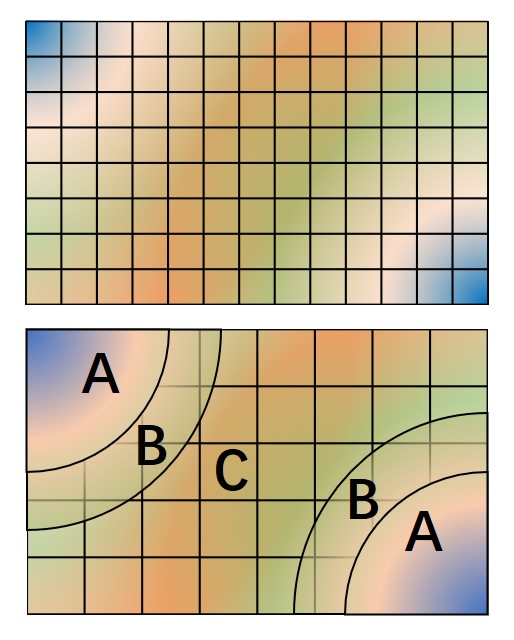
\includegraphics[trim={0 152 0 0},clip,width=0.45\columnwidth]{figures/hybrid_new.jpg}
\qquad
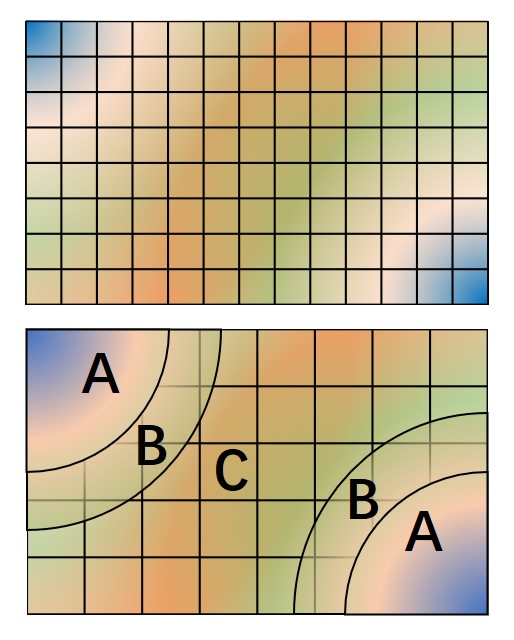
\includegraphics[trim={0 2 0 150},clip,width=0.45\columnwidth]{figures/hybrid_new.jpg}
\caption{Illustration of regular and hybrid orbital representation. Regular B-spline representation (left panel) contains only one region and a sufficiently fine mesh to resolve orbitals near the nucleus. The hybrid orbital representation (right panel) contains near nucleus (A) regions where spherical harmonics and radial functions are used, buffers (B) or interpolation regions, and an interstitial (C) region where a coarse B-spline mesh is utilized.}
\label{fig:hybridrep}
\end{figure}

To enable hybrid orbital representation, the input XML needs to see the tag \texttt{hybridrep="yes"} shown below.
\begin{lstlisting}[caption=Hybrid orbital representation input example.\label{listing:hybridrep}]
<determinantset type="bspline" source="i" href="pwscf.h5"
                tilematrix="1 1 3 1 2 -1 -2 1 0" twistnum="-1" gpu="yes" meshfactor="0.8"
                twist="0  0  0" precision="single" hybridrep="yes">
  ...
</determinantset>
\end{lstlisting}
Second, the infomation describing the atomic regions is required in the particle set, shown below
\begin{lstlisting}[caption=particleset elements for ions with information needed by hybrid orbital representation.\label{listing:hybridrep_particleset}]
  <group name="Ni">
    <parameter name="charge">          18 </parameter>
    <parameter name="valence">         18 </parameter>
    <parameter name="atomicnumber" >   28 </parameter>
    <parameter name="cutoff_radius" > 1.6 </parameter>
    <parameter name="inner_cutoff" >  1.3 </parameter>
    <parameter name="lmax" >            5 </parameter>
    <parameter name="spline_radius" > 1.8 </parameter>
    <parameter name="spline_npoints">  91 </parameter>
  </group>
\end{lstlisting}

The parameters specific to hybrid representation are listed as
\begin{table}[h]
\centering
\begin{tabularx}{\textwidth}{l l l l l l }
\hline
\multicolumn{6}{l}{\texttt{attrib} element} \\
\hline
\multicolumn{2}{l}{attribute      :} & \multicolumn{4}{l}{}\\
   &   \bfseries name            & \bfseries datatype & \bfseries values & \bfseries default   & \bfseries description \\
   &   \texttt{cutoff\_radius}             &  real            &  $>=0.0$    &  \textit{none}    & The cutoff radius for B/C boundary  \\
   &   \texttt{lmax}         &  integer            &  $>=0$ &  \textit{none} & Largetst angular channel \\
   &   \texttt{inner\_cutoff}             &  real            &  $>=0.0$    &  dep.    & The cutoff radius for A/B boundary  \\
   &   \texttt{spline\_radius}         &  real            &  $>0.0$ &  dep. & radial function radius used in spline \\
   &   \texttt{spline\_npoints}         &  integer            &  $>0$ &  dep. & Number of spline knots \\
  \hline
\end{tabularx}
\end{table}

\begin{itemize}
  \item \texttt{cutoff\_radius} is required for every species. If a species is intended not being covered by atomic regions, setting the value 0.0 will put default values for all the reset parameters. A good value is usually a bit larger than the core radius listed in the pseudopotential file. After a parametric scan, pick the one from the flat energy region with the smallest variance.
  \item \texttt{lmax} is required if $\texttt{cutoff\_radius} > 0.0$. The value usually needs to be at least the highest angular momentum plus 2.
  \item \texttt{inner\_cutoff} is optional and set as $\texttt{cutoff\_radius}-0.3$ by default which is fine in most cases.
  \item \texttt{spline\_radius} and \texttt{spline\_npoints} are optional. By default, they are calculated based on \texttt{cutoff\_radius} and a grid distplacement $0.02$\,bohr.
        If users prefer inputing them, it is required that $\texttt{cutoff\_radius}<=\texttt{spline\_radius}-2\times\texttt{spline\_radius}/(\texttt{spline\_npoints}-1)$.
\end{itemize}

In addition, the hybrid orbital representation allows extra optimization to speed up the non-local pseudopotential evaluation using the batched algorithm listed in Sec.~\ref{sec:nlpp}.

\include{spo_pw}
\include{spo_heg}


\input{jastrow}
\section{Multideterminant wavefunctions}
\label{sec:multideterminants}
Multiple schemes to generate a multideterminant wavefunction are
possible, from CASSF to full CI or selected CI. The \qmcpack converter can
convert MCSCF multideterminant wavefunctions from
GAMESS\cite{schmidt93} and CIPSI\cite{Caffarel2013} wavefunctions from
Quantum Package\cite{QP} (QP). Full details of how to run a CIPSI
calculation and convert the wavefunction for QMCPACK are given in 
Sec.~\ref{sec:cipsi}.


\input{backflow}

\chapter{Hamiltonian and Observables}
\label{chap:hamiltobs}


\qmcpack is capable of the simultaneous measurement of the Hamiltonian and many other quantum operators.  The Hamiltonian attains a special status among the available operators (also referred to as observables) because it ultimately generates all available information regarding the quantum system.  This is evident from an algorithmic standpoint as well since the Hamiltonian (embodied in the the projector) generates the imaginary time dynamics of the walkers in DMC and RMC. 

This section covers how the Hamiltonian can be specified, component by component, by the user in the XML format native to \qmcpack.  It also covers the input structure of statistical estimators corresponding to quantum observables such as the density, the static structure factor, and forces.



\section{The Hamiltonian}

The many-body Hamiltonian in Hartree units is given by
\begin{align}
  \hat{H} = -\sum_i\frac{1}{2m_i}\nabla_i^2 + \sum_iv^{ext}(r_i) + \sum_{i<j}v^{qq}(r_i,r_j)   + \sum_{i\ell}v^{qc}(r_i,r_\ell)   + \sum_{\ell<m}v^{cc}(r_\ell,r_m).  
\end{align}
Here, the sums indexed by $i/j$ are over quantum particles, while $\ell/m$ are reserved for classical particles.  Often the quantum particles are electrons and the classical particles are ions, though \qmcpack is not limited in this way.  The mass of each quantum particle is denoted $m_i$, $v^{qq}/v^{qc}/v^{cc}$ are pair potentials between quantum-quantum/quantum-classical/classical-classical particles, and $v^{ext}$ denotes a purely external potential.

\qmcpack is designed modularly so that any potential can be supported with minimal additions to the code base.  Potentials currently supported include Coulomb interactions in open and periodic boundary conditions, the modified periodic coulomb (MPC) potential, non-local pseudopotentials, helium pair potentials, and various model potentials such as hard sphere, gaussian, and modified Poschl-Teller.

Reference information and examples for the \texttt{<hamiltonian/>} XML element is provided below.  Detailed descriptions of the input for individual potentials is given in the sections that follow.  

% hamiltonian element
%  dev notes
%    Hamiltonian element read
%      HamiltonianPool::put
%        reads attributes: id name role target 
%          id/name is passed to QMCHamiltonian
%          role selects the primary hamiltonian
%          target associates to quantum particleset
%      HamiltonianFactory::build
%        reads attributes: type source default
%    HamiltonianFactory cloning may be flawed for non-electron systems
%      see HamiltonianFactory::clone
%        aCopy->renameProperty(``e'',qp->getName());
%        aCopy->renameProperty(psiName,psi->getName());
%      the renaming may not work if dynamic particleset.name!=''e''
%   lots of xml inputs are simply ignored if do not explicitly match (fix! here and elsewhere in the build tree)

\FloatBarrier
\begin{table}[h]
\begin{center}
\begin{tabularx}{\textwidth}{l l l l l l }
\hline
\multicolumn{6}{l}{\texttt{hamiltonian} element} \\
\hline
\multicolumn{2}{l}{parent elements:} & \multicolumn{4}{l}{\texttt{simulation, qmcsystem}}\\
\multicolumn{2}{l}{child  elements:} & \multicolumn{4}{l}{\texttt{pairpot extpot estimator constant}(deprecated)}\\
\multicolumn{2}{l}{attributes}  & \multicolumn{4}{l}{}\\
   &   \bfseries name     & \bfseries datatype & \bfseries values & \bfseries default & \bfseries description \\
   & \texttt{name/id}$^o$ &  text              & \textit{anything}& h0                & Unique id for this Hamiltonian instance  \\
   & \texttt{type}$^o$    &  text              &                  & generic           & \textit{No current function}             \\
   & \texttt{role}$^o$    &  text              & primary/extra    & extra             & Designate as primary Hamiltonian or not  \\
   & \texttt{source}$^o$  &  text              & \texttt{particleset.name} & i        & Identify classical particleset           \\
   & \texttt{target}$^o$  &  text              & \texttt{particleset.name} & e        & Identify quantum particleset             \\
   & \texttt{default}$^o$ &  boolean           & yes/no           & yes               & Include kinetic energy term implicitly   \\
  \hline
\end{tabularx}
\end{center}
\end{table}
\FloatBarrier

Additional information:
\begin{itemize}
  \item{\textbf{target:} Must be set to the name of the quantum particeset.  The default value is typically sufficient.  In normal usage, no other attributes are provided.}
\end{itemize}

% All-electron hamiltonian element
\begin{lstlisting}[caption=All electron Hamiltonian XML element.]
<hamiltonian target="e">
  <pairpot name="ElecElec" type="coulomb" source="e" target="e"/>
  <pairpot name="ElecIon"  type="coulomb" source="i" target="e"/>
  <pairpot name="IonIon"   type="coulomb" source="i" target="i"/>
</hamiltonian>
\end{lstlisting}


% Pseudopotential hamiltonian element
\begin{lstlisting}[caption=Pseudopotential Hamiltonian XML element.]
<hamiltonian target="e">
  <pairpot name="ElecElec"  type="coulomb" source="e" target="e"/>
  <pairpot name="PseudoPot" type="pseudo"  source="i" wavefunction="psi0" format="xml">
    <pseudo elementType="Li" href="Li.xml"/>
    <pseudo elementType="H" href="H.xml"/>
  </pairpot>
  <pairpot name="IonIon"    type="coulomb" source="i" target="i"/>
</hamiltonian>
\end{lstlisting}


\section{Pair potentials}

Many pair potentials are supported.  Though only the most commonly used pair potentials are covered in detail in this section, all currently available potentials are listed briefly below.  If a potential you desire is not covered below, or is not present at all, feel free to contact the developers.

% pairpot element
\FloatBarrier
\begin{table}[h]
\begin{center}
\begin{tabularx}{\textwidth}{l l l l l l }
\hline
\multicolumn{6}{l}{\texttt{pairpot} factory element} \\
\hline
\multicolumn{2}{l}{parent elements:} & \multicolumn{4}{l}{\texttt{hamiltonian}}\\
\multicolumn{2}{l}{type   selector:} & \multicolumn{4}{l}{\texttt{type} attribute}\\
\multicolumn{2}{l}{type   options: } & \multicolumn{2}{l}{coulomb           } & \multicolumn{2}{l}{Coulomb/Ewald potential}\\
\multicolumn{2}{l}{                } & \multicolumn{2}{l}{pseudo            } & \multicolumn{2}{l}{Semilocal pseudopotential}\\
\multicolumn{2}{l}{                } & \multicolumn{2}{l}{mpc               } & \multicolumn{2}{l}{Modified Periodic Coulomb interaction/correction}\\
\multicolumn{2}{l}{                } & \multicolumn{2}{l}{cpp               } & \multicolumn{2}{l}{Core polarization potential}\\
\multicolumn{2}{l}{                } & \multicolumn{2}{l}{numerical/*num*   } & \multicolumn{2}{l}{Numerical radial potential}\\
\multicolumn{2}{l}{                } & \multicolumn{2}{l}{skpot             } & \multicolumn{2}{l}{\textit{Unknown}}\\
\multicolumn{2}{l}{                } & \multicolumn{2}{l}{vhxc              } & \multicolumn{2}{l}{Exchange correlation potential (external)}\\
\multicolumn{2}{l}{                } & \multicolumn{2}{l}{jellium           } & \multicolumn{2}{l}{Atom-centered spherical jellium potential}\\
\multicolumn{2}{l}{                } & \multicolumn{2}{l}{hardsphere        } & \multicolumn{2}{l}{Hard sphere potential}\\
\multicolumn{2}{l}{                } & \multicolumn{2}{l}{gaussian          } & \multicolumn{2}{l}{Gaussian potential}\\
\multicolumn{2}{l}{                } & \multicolumn{2}{l}{modpostel         } & \multicolumn{2}{l}{Modified Poschl-Teller potential}\\
\multicolumn{2}{l}{                } & \multicolumn{2}{l}{huse              } & \multicolumn{2}{l}{Huse quintic potential}\\
\multicolumn{2}{l}{                } & \multicolumn{2}{l}{modInsKE          } & \multicolumn{2}{l}{Model insulator kinetic energy}\\
\multicolumn{2}{l}{                } & \multicolumn{2}{l}{oscillatory       } & \multicolumn{2}{l}{\textit{Unknown}}\\
\multicolumn{2}{l}{                } & \multicolumn{2}{l}{LJP\_smoothed     } & \multicolumn{2}{l}{Helium pair potential}\\
\multicolumn{2}{l}{                } & \multicolumn{2}{l}{HeSAPT\_smoothed  } & \multicolumn{2}{l}{Helium pair potential}\\
\multicolumn{2}{l}{                } & \multicolumn{2}{l}{HFDHE2\_Moroni1995} & \multicolumn{2}{l}{Helium pair potential}\\
\multicolumn{2}{l}{                } & \multicolumn{2}{l}{HFDHE2            } & \multicolumn{2}{l}{Helium pair potential}\\
\multicolumn{2}{l}{                } & \multicolumn{2}{l}{eHe               } & \multicolumn{2}{l}{Helium-electron pair potential}\\
\multicolumn{2}{l}{shared attributes:} & \multicolumn{4}{l}{}\\
   &   \bfseries name     & \bfseries datatype & \bfseries values & \bfseries default   & \bfseries description \\
   &   \texttt{type}$^r$      &  text              & \textit{See above}        & 0                   & Select pairpot type         \\
   &   \texttt{name}$^r$      &  text              & \textit{anything}         & any                 & Unique name for this pairpot\\
   &   \texttt{source}$^r$    &  text              & \texttt{particleset.name} &\texttt{hamiltonian.target}& Identify interacting particles\\
   &   \texttt{target}$^r$    &  text              & \texttt{particleset.name} &\texttt{hamiltonian.target}& Identify interacting particles  \\
   &   \texttt{units}$^o$     &  text              &                           & hartree             & \textit{No current function}  \\
\hline
\end{tabularx}
\end{center}
\end{table}
\FloatBarrier

Additional information:
\begin{itemize}
  \item{\textbf{type:} Used to select the desired pair potential.  Must be selected from the list of type options above.}
  \item{\textbf{name:} A unique name used to identify this pair potential.  Block averaged output data will appear under this name in \texttt{scalar.dat} and/or \texttt{stat.h5} files.}
  \item{\textbf{source/target:}  These specify the particles involved in a pair interaction.  If an interaction is between classical (e.g. ions) and quantum (e.g. electrons), \texttt{source}/\texttt{target} should be the name of the classical/quantum particleset.}
  \item{Only \texttt{coulomb, pseudo, mpc} are described in detail below.  The older or less used types (\texttt{cpp, numerical, jellium, hardsphere, gaussian, huse, modpostel, oscillatory, skpot, vhxc, modInsKE, LJP\_smoothed, HeSAPT\_smoothed, HFDHE2\_Moroni1995, eHe, HFDHE2}) are not covered.}
  \dev{
  \item{Available only if \texttt{QMC\_BUILD\_LEVEL>2} and \texttt{QMC\_CUDA} is not defined: \texttt{hardsphere, gaussian, huse, modpostel, oscillatory, skpot}.}
  \item{Available only if \texttt{OHMMS\_DIM==3}: \texttt{mpc, vhxc, pseudo}.}
  \item{Available only if \texttt{OHMMS\_DIM==3} and \texttt{QMC\_BUILD\_LEVEL>2} and \texttt{QMC\_CUDA} is not defined: \texttt{cpp, LJP\_smoothed, HeSAPT\_smoothed, HFDHE2\_Moroni1995, eHe, jellium, HFDHE2, modInsKE}.}
  }
\end{itemize}


% physical read by coulomb potentials
% potential is only for pressure estimator



% pairpot instances

%   do coulomb, pseudo, mpc

\subsection{Coulomb potentials}

The bare Coulomb potential is used in open boundary conditions:
\begin{align}
  V_c^{open} = \sum_{i<j}\frac{q_iq_j}{\abs{r_i-r_j}}
\end{align}

When periodic boundary conditions are selected, Ewald summation is used automatically:
\begin{align}\label{eq:ewald}
  V_c^{pbc} = \sum_{i<j}\frac{q_iq_j}{\abs{r_i-r_j}} + \frac{1}{2}\sum_{L\ne0}\sum_{i,j}\frac{q_iq_j}{\abs{r_i-r_j+L}}
\end{align}
The sum indexed by $L$ is over all non-zero simulation cell lattice vectors.  In practice, the Ewald sum is broken into short and long ranged parts in a manner optimized for efficiency (see Ref. \cite{Natoli1995}) for details. 

For information on how to set the boundary conditions, consult Sec. \ref{chap:simulationcell}.


\FloatBarrier
\begin{table}[h]
\begin{center}
\begin{tabularx}{\textwidth}{l l l l l l }
\hline
\multicolumn{6}{l}{\texttt{pairpot type=coulomb} element} \\
\hline
\multicolumn{2}{l}{parent elements:} & \multicolumn{4}{l}{\texttt{hamiltonian}}\\
\multicolumn{2}{l}{child  elements:} & \multicolumn{4}{l}{\textit{None}}\\
\multicolumn{2}{l}{attributes}  & \multicolumn{4}{l}{}\\
   &   \bfseries name     & \bfseries datatype & \bfseries values & \bfseries default   & \bfseries description \\
   & \texttt{type}$^r$    &  text              & \textbf{coulomb} &                     & Must be coulomb     \\
   & \texttt{name/id}$^r$ &  text              & \textit{anything}&  ElecElec           & Unique name for interaction\\
   & \texttt{source}$^r$  &  text              & \texttt{particleset.name} &\texttt{hamiltonian.target}& Identify interacting particles\\
   & \texttt{target}$^r$  &  text              & \texttt{particleset.name} &\texttt{hamiltonian.target}& Identify interacting particles\\
   & \texttt{pbc}$^o$     &  boolean           & yes/no           & yes                 & Use Ewald summation  \\
   & \texttt{physical}$^o$&  boolean           & yes/no           & yes                 & Hamiltonian(yes)/observable(no) \\
\dev{& \texttt{forces}      &  boolean           & yes/no           & no                  & \textit{Deprecated}             \\ }
  \hline
\end{tabularx}
\end{center}
\end{table}
\FloatBarrier

Additional information
\begin{itemize}
  \item{\textbf{type/source/target} See description for the generic \texttt{pairpot} factory element above.}
  \item{\textbf{name:} Traditional user-specified names for electron-electron, electron-ion, and ion-ion terms are \texttt{ElecElec}, \texttt{ElecIon}, and \texttt{IonIon}, respectively.  While any choice can be used, the data analysis tools expect to find columns in \texttt{*.scalar.dat} with these names.}
  \item{\textbf{pbc}: Ewald summation will not be performed if \texttt{simulationcell.bconds== n n n}, regardless of the value of \texttt{pbc}.  Similarly, the \texttt{pbc} attribute can only be used to turn off Ewald summation if \texttt{simulationcell.bconds!= n n n}.  The default value is recommended.}
  \item{\textbf{physical}: If \texttt{physical==yes}, this pair potential is included in the Hamiltonian and will factor into the \texttt{LocalEnergy} reported by QMCPACK and also in the DMC branching weight.  If \texttt{physical==no}, then the pair potential is treated as a passive observable but not as part of the Hamiltonian itself.  As such it does not contribute to the outputted \texttt{LocalEnergy}.  Regardless of the value of \texttt{physical} output data will appear in \texttt{scalar.dat} in a column headed by \texttt{name}.}
\end{itemize}


\begin{lstlisting}[caption=XML element for Coulomb interaction between electrons.]
  <pairpot name="ElecElec" type="coulomb" source="e" target="e"/>
\end{lstlisting}

\begin{lstlisting}[caption=XML element for Coulomb interaction between electrons and ions (all-electron only).]
  <pairpot name="ElecIon"  type="coulomb" source="i" target="e"/>
\end{lstlisting}

\begin{lstlisting}[caption=XML element for Coulomb interaction between ions.]
  <pairpot name="IonIon"   type="coulomb" source="i" target="i"/>
\end{lstlisting}


\subsection{Pseudopotentials}
\label{sec:nlpp}
\qmcpack supports pseudopotentials in semilocal form, which is local in the radial coordinate and non-local in angular coordinates.  When all angular momentum channels above a certain threshold ($\ell_{max}$) are well approximated by the same potential ($V_{\bar{\ell}}\equiv V_{loc}$), the pseudpotential separates into a fully local channel and an angularly-nonlocal component:
\begin{align}
  V^{PP} = \sum_{ij}\Big(V_{\bar{\ell}}(\abs{r_i-\tilde{r}_j}) + \sum_{\ell\ne\bar{\ell}}^{\ell_{max}}\sum_{m=-\ell}^\ell \operator{Y_{\ell m}}{\big[V_\ell(\abs{r_i-\tilde{r}_j}) - V_{\bar{\ell}}(\abs{r_i-\tilde{r}_j}) \big]}{Y_{\ell m}} \Big)
\end{align}  
Here the electron/ion index is $i/j$ and only one type of ion is shown for simplicity.

Evaluation of the localized pseudopotential energy $\Psi_T^{-1}V^{PP}\Psi_T$ requires additional angular integrals.  These integrals are evaluated on a randomly shifted angular grid.  The size of this grid is determined by $\ell_{max}$.  See Ref. \cite{Mitas1991} for further detail. 

\qmcpack uses the FSAtom pseudopotential file format associated with the ``Free Software Project for Atomic-scale Simulations'' initiated in 2002  (see \url{http://www.tddft.org/fsatom/manifest.php} for general information).  The FSAtom format uses XML for structured data.  Files in this format do not use a specific identifying file extension; they are simply suffixed with ``\texttt{.xml}''.  The tabular data format of CASINO is also supported.


% FSAtom format links
%   unfortunately none of the surviving links detail the format itself
% http://www.tddft.org/fsatom/index.php
% http://www.tddft.org/fsatom/programs.php
% http://www.tddft.org/fsatom/manifest.php
% http://163.13.111.58/cchu/reference/web/PseudoPotentials%20-%20FSAtom%20Wiki.htm
% http://departments.icmab.es/leem/alberto/xml/pseudo/index.html



% pseudopotential element
%   dev notes
%     attributes name, source, wavefunction, format are read in CoulombFactory.cpp  HamiltonianFactory::addPseudoPotential
%     format==''old'' refers to an old table format that is no longer supported
%     read continues in ECPotentialBuilder::put()
%       if format!=xml/old (i.e. table) qmcpack will attempt to read from *.psf files
%         in this case, <pairpot type=''pseudo'' format=''table''/>, ie there are no elements
%         if particlset groups are Li H (in order), then it looks for Li.psf and H.psf
%         what is the psf format?
%       if format==xml, normal read continues, i.e. <pseudo/> child elements are expected
%         read is not sensitive to particleset group/species ordering
%         child elements not named <pseudo/> are simply ignored (FIX!)
\FloatBarrier
\begin{table}[h]
\begin{center}
\begin{tabularx}{\textwidth}{l l l l l l }
\hline
\multicolumn{6}{l}{\texttt{pairpot type=pseudo} element} \\
\hline
\multicolumn{2}{l}{parent elements:} & \multicolumn{4}{l}{\texttt{hamiltonian}}\\
\multicolumn{2}{l}{child  elements:} & \multicolumn{4}{l}{\texttt{pseudo}}\\
\multicolumn{2}{l}{attributes}  & \multicolumn{4}{l}{}\\
   &   \bfseries name     & \bfseries datatype & \bfseries values & \bfseries default   & \bfseries description \\
   & \texttt{type}$^r$    &  text              & \textbf{pseudo} &                      & Must be pseudo         \\
   & \texttt{name/id}$^r$ &  text              & \textit{anything}&  PseudoPot          & \textit{No current function}\\
   & \texttt{source}$^r$  &  text              & \texttt{particleset.name} &  i                  & Ion particleset name\\
   & \texttt{target}$^r$  &  text              & \texttt{particleset.name} &\texttt{hamiltonian.target}& Electron particleset name  \\
   & \texttt{pbc}$^o$     &  boolean           & yes/no           & yes$^*$             & Use Ewald summation  \\
   & \texttt{forces}      &  boolean           & yes/no           & no                  & \textit{Deprecated}             \\
   &\texttt{wavefunction}$^r$ &  text          & \texttt{wavefunction.name}& invalid    & Identify wavefunction \\
   &   \texttt{format}$^r$    &  text          & xml/table        & table               & Select file format   \\
   & \texttt{algorithm}$^o$   &  text          & batched/default  & default             & Choose NLPP algorithm \\
  \hline
\end{tabularx}
\end{center}
\end{table}
\FloatBarrier

Additional information:
\begin{itemize}
  \item{\textbf{type/source/target} See description for the generic \texttt{pairpot} factory element above.}
  \item{\textbf{name:} Ignored.  Instead default names will be present in \texttt{*scalar.dat} output files when pseudopotentials are used.  The field \texttt{LocalECP} refers to the local part of the pseudopotential.  If non-local channels are present, a \texttt{NonLocalECP} field will be added that contains the non-local energy summed over all angular momentum channels.}
  \item{\textbf{pbc:} Ewald summation will not be performed if \texttt{simulationcell.bconds== n n n}, regardless of the value of \texttt{pbc}.  Similarly, the \texttt{pbc} attribute can only be used to turn off Ewald summation if \texttt{simulationcell.bconds!= n n n}.}
  \item{\textbf{format:}  If \texttt{format}==table, QMCPACK looks for \texttt{*.psf} files containing pseudopotential data in a tabular format.  The files must be named after the ionic species provided in \texttt{particleset} (\emph{e.g.} \texttt{Li.psf} and \texttt{H.psf}). If \texttt{format}==xml, additional \texttt{pseudo} child XML elements must be provided (see below).  These elements specify individual file names and formats (both the FSAtom XML and CASINO tabular data formats are supported). }
  \item{\textbf{algorithm} The default algorithm evaluates the ratios of wavefunction components together for each qudarature point and then one point after another. The batched algorithm evaluates the ratios of qudarature points together for each wavefunction component and then one component after another. Internally, it uses VirtualParticleSet for quadrature points. Hybrid orbital representation has an extra optimization enabled when using the batched algorithm.}
\end{itemize}


\begin{lstlisting}[caption=XML element for pseudopotential electron-ion interaction (psf files).]
  <pairpot name="PseudoPot" type="pseudo"  source="i" wavefunction="psi0" format="psf"/>
\end{lstlisting}

\begin{lstlisting}[caption=XML element for pseudopotential electron-ion interaction (xml files).]
  <pairpot name="PseudoPot" type="pseudo"  source="i" wavefunction="psi0" format="xml">
    <pseudo elementType="Li" href="Li.xml"/>
    <pseudo elementType="H" href="H.xml"/>
  </pairpot>
\end{lstlisting}

%\begin{lstlisting}[caption=XML element for pseudopotential electron-ion interaction (CASINO files).]
%  <pairpot name="PseudoPot" type="pseudo"  source="i" wavefunction="psi0" format="xml">
%    <pseudo elementType="Li" href="Li.data"/>
%    <pseudo elementType="H" href="H.data"/>
%  </pairpot>
%\end{lstlisting}


Details of \texttt{<pseudo/>} input elements are given below.  It is possible to include (or construct) a full pseudopotential directly in the input file without providing an external file via \texttt{href}.  The full XML format for pseudopotentials is not yet covered.

% pseudo element
%   dev notes
%     initial read of href elementType/symbol attributes at ECPotentialBuilder::useXmlFormat()
%     read continues in ECPComponentBuilder
%       format==xml and href==none (not provided) => ECPComponentBuilder::put(cur)
%       format==xml and href==a file => ECPComponentBuilder::parse(href,cur)
%       format==casino => ECPComponentBuilder::parseCasino(href,cur)
%         this reader is tucked away in ECPComponentBuilder.2.cpp
%         nice demonstration of OhmmsAsciiParser here
%         maximum cutoff defined by a 1.e-5 (Ha?) spread in the nonlocal potentials
%     quadrature rules (1-7) set as in J. Chem. Phys. 95 (3467) (1991), see below
%       Rule     # points     lexact
%        1           1          0
%        2           4          2
%        3           6          3
%        4          12          5
%        5          18          5
%        6          26          7
%        7          50         11
%     looks like channels only go from s-g (see ECPComponentBuilder constructor)
%       perhaps not, quadrature rules really do go up to 7 (lexact==11), see SetQuadratureRule()
\FloatBarrier
\begin{table}[h]
\begin{center}
\begin{tabularx}{\textwidth}{l l l l l l }
\hline
\multicolumn{6}{l}{\texttt{pseudo} element} \\
\hline
\multicolumn{2}{l}{parent elements:} & \multicolumn{4}{l}{\texttt{pairpot type=pseudo}}\\
\multicolumn{2}{l}{child  elements:} & \multicolumn{4}{l}{\texttt{header local grid}}\\
\multicolumn{2}{l}{attributes}  & \multicolumn{4}{l}{}\\
   &   \bfseries name     & \bfseries datatype & \bfseries values & \bfseries default   & \bfseries description \\
   & \texttt{elementType/symbol}$^r$&  text    &\texttt{group.name}& none               & Identify ionic species   \\
   & \texttt{href}$^r$    &  text              & \textit{filepath}& none                & Pseudopotential file path\\
   & \texttt{format}$^r$  &  text              & xml/casino       & xml                 & Specify file format\\
   & \texttt{cutoff}$^o$  &  real              &                  &                     & Non-local cutoff radius  \\
   & \texttt{lmax}$^o$    &  integer           &                  &                     & Largest angular momentum  \\
   & \texttt{nrule}$^o$   &  integer           &                  &                     & Integration grid order             \\
  \hline
\end{tabularx}
\end{center}
\end{table}
\FloatBarrier


\begin{lstlisting}[caption=XML element for pseudopotential of single ionic species.]
  <pseudo elementType="Li" href="Li.xml"/>
\end{lstlisting}



\subsection{Modified periodic Coulomb interaction/correction}

The modified periodic Coulomb (MPC) interaction is an alternative to direct Ewald summation.  The MPC corrects the exchange correlation hole to more closely match its thermodynamic limit.  Because of this, the MPC exhibits smaller finite size errors than the bare Ewald interaction, though a few alternative and competitive finite size correction schemes now exist.  The MPC is itself often used just as a finite size correction in postprocessing (set \texttt{physical=false} in the input).  


% mpc element
%  dev notes
%    most attributes are read in CoulombPotentialFactory.cpp  HamiltonianFactory::addMPCPotential()
%    user input for the name attribute is ignored and the name is always MPC
%    density G-vectors are stored in ParticleSet: Density_G and DensityReducedGvecs members
%    check the Linear Extrap and Quadratic Extrap output in some real examples (see MPC::init_f_G())
%      what are acceptable values for the discrepancies?
%      check that these decrease as cutoff is increased 
%    commented out code for MPC.dat creation in MPC::initBreakup()
%    short range part is 1/r, MPC::evalSR()
%    long range part is on a spline (VlongSpline), MPC::evalLR()
\FloatBarrier
\begin{table}[h]
\begin{center}
\begin{tabularx}{\textwidth}{l l l l l l }
\hline
\multicolumn{6}{l}{\texttt{pairpot type=mpc} element} \\
\hline
\multicolumn{2}{l}{parent elements:} & \multicolumn{4}{l}{\texttt{hamiltonian}}\\
\multicolumn{2}{l}{child  elements:} & \multicolumn{4}{l}{\textit{None}}\\
\multicolumn{2}{l}{attributes}  & \multicolumn{4}{l}{}\\
   &   \bfseries name     & \bfseries datatype & \bfseries values & \bfseries default   & \bfseries description \\
   & \texttt{type}$^r$    &  text              & \textbf{mpc}     &                     & Must be mpc         \\
   & \texttt{name/id}$^r$ &  text              & \textit{anything}&  MPC                & Unique name for interaction \\
   & \texttt{source}$^r$  &  text              & \texttt{particleset.name} &\texttt{hamiltonian.target}& Identify interacting particles\\
   & \texttt{target}$^r$  &  text              & \texttt{particleset.name} &\texttt{hamiltonian.target}& Identify interacting particles  \\
   & \texttt{physical}$^o$&  boolean           & yes/no           & no                  & Hamiltonian(yes)/observable(no) \\
   &  \texttt{cutoff}     &  real              & $>0$             & 30.0                & Kinetic energy cutoff \\
  \hline
\end{tabularx}
\end{center}
\end{table}
\FloatBarrier
Remarks
\begin{itemize}
  \item{\texttt{physical}:  Typically set to \texttt{no}, meaning the standard Ewald interaction will be used during sampling and MPC will be measured as an observable for finite-size post correction.  If \texttt{physical} is \texttt{yes}, the MPC interaction will be used during sampling.  In this case an electron-electron Coulomb \texttt{pairpot} element should not be supplied.}
  \item{Developer note: Currently the \texttt{name} attribute for the mpc interaction is ignored.  The name is always reset to \texttt{MPC}.}
\end{itemize}

% MPC correction
\begin{lstlisting}[caption=Modified periodic coulomb for finite size post-correction.]
  <pairpot type="MPC" name="MPC" source="e" target="e" ecut="60.0" physical="no"/>
\end{lstlisting}



% estimator element
\section{General estimators}

A broad range of estimators for physical observables are available in \qmcpack.  The sections below contain input details for the total number density (\texttt{density}), number density resolved by particle spin (\texttt{spindensity}), spherically averaged pair correlation function (\texttt{gofr}), static structure factor (\texttt{sk}), energy density (\texttt{energydensity}), one body reduced density matrix (\texttt{dm1b}), $S(k)$ based kinetic energy correction (\texttt{chiesa}), forward walking (\texttt{ForwardWalking}), and force (\texttt{Force}) estimators.  Other estimators are not yet covered.

When an \texttt{<estimator/>} element appears in \texttt{<hamiltonian/>}, it is evaluated for all applicable chained QMC runs (\emph{e.g.} VMC$\rightarrow$DMC$\rightarrow$DMC).  Estimators are generally not accumulated during wavefunction optimization sections.    If an \texttt{<estimator/>} element is instead provided in a particular \texttt{<qmc/>} element, that estimator is only evaluated for that specific section (\textit{e.g.} during VMC only).


\FloatBarrier
\begin{table}[h]
\begin{center}
\begin{tabularx}{\textwidth}{l l l l l l }
\hline
\multicolumn{6}{l}{\texttt{estimator} factory element} \\
\hline
\multicolumn{2}{l}{parent elements:} & \multicolumn{4}{l}{\texttt{hamiltonian, qmc}}\\
\multicolumn{2}{l}{type   selector:} & \multicolumn{4}{l}{\texttt{type} attribute}\\
\multicolumn{2}{l}{type   options: } & \multicolumn{2}{l}{density           } & \multicolumn{2}{l}{Density on a grid}\\
\multicolumn{2}{l}{                } & \multicolumn{2}{l}{spindensity       } & \multicolumn{2}{l}{Spin density on a grid}\\
\multicolumn{2}{l}{                } & \multicolumn{2}{l}{gofr              } & \multicolumn{2}{l}{Pair correlation function (quantum species)}\\
\multicolumn{2}{l}{                } & \multicolumn{2}{l}{sk                } & \multicolumn{2}{l}{Static structure factor}\\
\multicolumn{2}{l}{                } & \multicolumn{2}{l}{structurefactor   } & \multicolumn{2}{l}{Species resolved structure factor}\\
\multicolumn{2}{l}{                } & \multicolumn{2}{l}{momentum          } & \multicolumn{2}{l}{Momentum distribution}\\
\multicolumn{2}{l}{                } & \multicolumn{2}{l}{energydensity     } & \multicolumn{2}{l}{Energy density on uniform or Voronoi grid}\\
\multicolumn{2}{l}{                } & \multicolumn{2}{l}{dm1b              } & \multicolumn{2}{l}{One body density matrix in arbitrary basis}\\
\multicolumn{2}{l}{                } & \multicolumn{2}{l}{chiesa            } & \multicolumn{2}{l}{Chiesa-Ceperley-Martin-Holzmann kinetic energy correction}\\
\multicolumn{2}{l}{                } & \multicolumn{2}{l}{Force             } & \multicolumn{2}{l}{Family of ``force'' estimators (see \ref{sec:force_est})}\\
\multicolumn{2}{l}{                } & \multicolumn{2}{l}{ForwardWalking    } & \multicolumn{2}{l}{Forward walking values for existing estimators}\\
\multicolumn{2}{l}{                } & \multicolumn{2}{l}{orbitalimages     } & \multicolumn{2}{l}{Create image files for orbitals, then exit}\\
\multicolumn{2}{l}{                } & \multicolumn{2}{l}{flux              } & \multicolumn{2}{l}{Checks sampling of kinetic energy}\\
\multicolumn{2}{l}{                } & \multicolumn{2}{l}{localmoment       } & \multicolumn{2}{l}{Atomic spin polarization within cutoff radius}\\
\multicolumn{2}{l}{                } & \multicolumn{2}{l}{numberfluctuations} & \multicolumn{2}{l}{Spatial number fluctuations}\\
\multicolumn{2}{l}{                } & \multicolumn{2}{l}{HFDHE2            } & \multicolumn{2}{l}{Helium pressure}\\
\multicolumn{2}{l}{                } & \multicolumn{2}{l}{NearestNeighbors  } & \multicolumn{2}{l}{Trace nearest neighbor indices}\\
\dev{
\multicolumn{2}{l}{                } & \multicolumn{2}{l}{Kinetic           } & \multicolumn{2}{l}{\textit{No current function}}\\
\multicolumn{2}{l}{                } & \multicolumn{2}{l}{Pressure          } & \multicolumn{2}{l}{\textit{No current function}}\\
\multicolumn{2}{l}{                } & \multicolumn{2}{l}{ZeroVarObs        } & \multicolumn{2}{l}{\textit{No current function}}\\
\multicolumn{2}{l}{                } & \multicolumn{2}{l}{DMCCorrection     } & \multicolumn{2}{l}{\textit{No current function}}\\
\multicolumn{2}{l}{shared attributes:} & \multicolumn{4}{l}{}\\
}
   &   \bfseries name     & \bfseries datatype & \bfseries values & \bfseries default   & \bfseries description \\
   &   \texttt{type}$^r$      &  text              & \textit{See above}        & 0                   & Select estimator type         \\
   &   \texttt{name}$^r$      &  text              & \textit{anything}         & any                 & Unique name for this estimator\\
   %&   \texttt{source}$^r$    &  text              & \texttt{particleset.name} &\texttt{hamiltonian.target}& Identify interacting particles\\
   %&   \texttt{target}$^r$    &  text              & \texttt{particleset.name} &\texttt{hamiltonian.target}& Identify interacting particles  \\
   %&   \texttt{units}$^o$     &  text              &                           & hartree             & \textit{No current function}  \\
\hline
\end{tabularx}
\end{center}
\end{table}
\FloatBarrier


%  <estimator type="structurefactor" name="StructureFactor" report="yes"/>
%  <estimator type="nofk" name="nofk" wavefunction="psi0"/>


%\dev{
%\FloatBarrier
%\begin{table}[h]
%\begin{center}
%\begin{tabularx}{\textwidth}{l l l l l l }
%\hline
%\multicolumn{6}{l}{\texttt{estimator type=X} element} \\
%\hline
%\multicolumn{2}{l}{parent elements:} & \multicolumn{4}{l}{\texttt{hamiltonian, qmc}}\\
%\multicolumn{2}{l}{child  elements:} & \multicolumn{4}{l}{\textit{None}}\\
%\multicolumn{2}{l}{attributes}  & \multicolumn{4}{l}{}\\
%   &   \bfseries name     & \bfseries datatype & \bfseries values & \bfseries default   & \bfseries description \\
%   & \texttt{type}$^r$    &  text              & \textbf{X}     &                     & Must be X         \\
%   & \texttt{name}$^r$    &  text              & \textit{anything}&                  & Unique name for estimator \\
%   & \texttt{source}$^o$  &  text              & \texttt{particleset.name} &\texttt{hamiltonian.target}& Identify particles\\
%   & \texttt{target}$^o$  &  text              & \texttt{particleset.name} &\texttt{hamiltonian.target}& Identify particles  \\
%  \hline
%\end{tabularx}
%\end{center}
%\end{table}
%\FloatBarrier
%}


\subsection{Chiesa-Ceperley-Martin-Holzmann kinetic energy correction}

This estimator calculates a finite size correction to the kinetic energy following the formalism laid out in Ref. \cite{Chiesa2006}.  The total energy can be corrected for finite size effects by using this estimator in conjuction with the MPC correction.

\FloatBarrier
\begin{table}[h]
\begin{center}
\begin{tabularx}{\textwidth}{l l l l l l }
\hline
\multicolumn{6}{l}{\texttt{estimator type=chiesa} element} \\
\hline
\multicolumn{2}{l}{parent elements:} & \multicolumn{4}{l}{\texttt{hamiltonian, qmc}}\\
\multicolumn{2}{l}{child  elements:} & \multicolumn{4}{l}{\textit{None}}\\
\multicolumn{2}{l}{attributes}  & \multicolumn{4}{l}{}\\
   &   \bfseries name     & \bfseries datatype & \bfseries values & \bfseries default   & \bfseries description \\
   & \texttt{type}$^r$    &  text              & \textbf{chiesa}            &        & Must be chiesa         \\
   & \texttt{name}$^o$    &  text              & \textit{anything}          & KEcorr & Always reset to KEcorr \\
   & \texttt{source}$^o$  &  text              & \texttt{particleset.name}  & e      & Identify quantum particles\\
   & \texttt{psi}$^o$     &  text              & \texttt{wavefunction.name} & psi0   & Identify wavefunction  \\
  \hline
\end{tabularx}
\end{center}
\end{table}
\FloatBarrier

% kinetic energy correction
\begin{lstlisting}[caption=``Chiesa'' kinetic energy finite size post-correction.]
   <estimator name="KEcorr" type="chiesa" source="e" psi="psi0"/>
\end{lstlisting}




\subsection{Density estimator}
The particle number density operator is given by
\begin{align}
  \hat{n}_r = \sum_i\delta(r-r_i)
\end{align}
The \texttt{density} estimator accumulates the number density on a uniform histogram grid over the simulation cell.  The value obtained for a grid cell $c$ with volume $\Omega_c$ is then the average number of particles in that cell:
\begin{align}
  n_c = \int dR \abs{\Psi}^2 \int_{\Omega_c}dr \sum_i\delta(r-r_i)
\end{align}  


\FloatBarrier
\begin{table}[h]
\begin{center}
\begin{tabularx}{\textwidth}{l l l l l l }
\hline
\multicolumn{6}{l}{\texttt{estimator type=density} element} \\
\hline
\multicolumn{2}{l}{parent elements:} & \multicolumn{4}{l}{\texttt{hamiltonian, qmc}}\\
\multicolumn{2}{l}{child  elements:} & \multicolumn{4}{l}{\textit{None}}\\
\multicolumn{2}{l}{attributes}  & \multicolumn{4}{l}{}\\
   &   \bfseries name     & \bfseries datatype & \bfseries values  & \bfseries default   & \bfseries description \\
   & \texttt{type}$^r$      &  text              & \textbf{density}      &                     & Must be density         \\
   & \texttt{name}$^r$      &  text              & \textit{anything}     & any                 & Unique name for estimator \\
   & \texttt{delta}$^o$     &  real array(3)     & $0\le v_i \le 1$      & 0.1 0.1 0.1         & Grid cell spacing, unit coords\\
   & \texttt{x\_min}$^o$    &  real              & $>0$                  & 0                   & Grid starting point in x (Bohr)\\
   & \texttt{x\_max}$^o$    &  real              & $>0$                  &$|\texttt{lattice[0]}|$& Grid ending point in x (Bohr)\\
   & \texttt{y\_min}$^o$    &  real              & $>0$                  & 0                   & Grid starting point in y (Bohr)\\
   & \texttt{y\_max}$^o$    &  real              & $>0$                  &$|\texttt{lattice[1]}|$& Grid ending point in y (Bohr)\\
   & \texttt{z\_min}$^o$    &  real              & $>0$                  & 0                   & Grid starting point in z (Bohr)\\
   & \texttt{z\_max}$^o$    &  real              & $>0$                  &$|\texttt{lattice[2]}|$& Grid ending point in z (Bohr)\\
   & \texttt{potential}$^o$ &  boolean           & yes/no                & no                  & Accumulate local potential, \textit{Deprecated}\\
   & \texttt{debug}$^o$     &  boolean           & yes/no                & no                  & \textit{No current function}\\
  \hline
\end{tabularx}
\end{center}
\end{table}
\FloatBarrier


Additional information:
\begin{itemize}
  \item{\texttt{name}: The name provided will be used as a label in the \texttt{stat.h5} file for the blocked output data.  Post-processing tools expect \texttt{name="Density"}.}
  \item{\texttt{delta}:  This sets the histogram grid size used to accumulate the density: \texttt{delta="0.1 0.1 0.05"}$\rightarrow 10\times 10\times 20$ grid, \texttt{delta="0.01 0.01 0.01"}$\rightarrow 100\times 100\times 100$ grid.  The density grid is written to a \texttt{stat.h5} file at the end of each Monte Carlo block.  If you request many $blocks$ in a \texttt{<qmc/>} element, or select a large grid, the resulting \texttt{stat.h5} file may be many GB in size.}
  \item{\texttt{*\_min/*\_max}: Can be used to select a subset of the simulation cell for the density histogram grid.  For example if a (cubic) simulation cell is 20 Bohr on a side, setting \texttt{*\_min=5.0} and \texttt{*\_max=15.0} will result in a density histogram grid spanning a $10\times 10\times 10$ Bohr cube about the center of the box.  Use of \texttt{x\_min, x\_max, y\_min, y\_max, z\_min, z\_max} is only appropriate for orthorhombic simulation cells with open boundary conditions.}
  \item{When open boundary conditions are used, a \texttt{<simulationcell/>} element must be explicitly provided as the first sub-element of \texttt{<qmcsystem/>} for the density estimator to work.  In this case the molecule should be centered around the middle of the simulation cell ($L/2$) and not the origin ($0$} since the space within the cell, and hence the density grid, is defined from $0$ to $L$.
\end{itemize}


% density estimator
\begin{lstlisting}[caption=Density estimator (uniform grid).]
   <estimator name="Density" type="density" delta="0.05 0.05 0.05"/>
\end{lstlisting}

\subsection{Lattice deviation estimator}
Record deviation of a group of particles in one particle set (target) from a group of particles in another particle set (source).

\FloatBarrier
\begin{table}[h]
\begin{center}
\begin{tabularx}{\textwidth}{l l l l l l }
\hline
\multicolumn{6}{l}{\texttt{estimator type=sk} element} \\
\hline
\multicolumn{2}{l}{parent elements:} & \multicolumn{4}{l}{\texttt{hamiltonian, qmc}}\\
\multicolumn{2}{l}{child  elements:} & \multicolumn{4}{l}{\textit{None}}\\
\multicolumn{2}{l}{attributes}  & \multicolumn{4}{l}{}\\
   & \bfseries name       & \bfseries datatype & \bfseries values  & \bfseries default   & \bfseries description \\
   & \texttt{type}$^r$    &  text              & latticedeviation      &                     & Must be latticedeviation       \\
   & \texttt{name}$^r$    &  text              & \textit{anything} & any                 & Unique name for estimator \\
   & \texttt{hdf5}$^o$    &  boolean           & yes/no            & no                  & Output to \texttt{stat.h5} (yes) \\
   & \texttt{per\_xyz}$^o$    &  boolean           & yes/no            & no                  & Directional-resolved (yes) \\
   & \texttt{source}$^r$    &  text           & e/ion0/\dots         & no                  & source particle set \\
   & \texttt{sgroup}$^r$    &  text           & u/d/\dots         & no                  & source particle group \\
   & \texttt{target}$^r$    &  text           & e/ion0/\dots         & no                  & target particle set \\
   & \texttt{tgroup}$^r$    &  text           & u/d/\dots         & no                  & target particle group \\
  \hline
\end{tabularx}
\end{center}
\end{table}
\FloatBarrier

Additional information:
\begin{itemize}
  \item{\texttt{source}: The ``reference'' particle set to measure distances from, actual reference points are determined together with \verb|sgroup|.}
  \item{\texttt{sgroup}: The ``reference'' particle group to measure distances from.} 
  \item{\texttt{source}: The ``target'' particle set to measure distances to.}
  \item{\texttt{sgroup}: The ``target'' particle group to measure distances to. For example, in Listing~\ref{lst:latdev}, the distance from the up electron (``u'') to the origin of the coordinate system is recorded.}
  \item{\texttt{per\_xyz}: Record direction-resolved distance. In Listing~\ref{lst:latdev}, the x,y,z coordinates of the up electron will be recorded separately if \texttt{per\_xyz=yes}.}
  \item{\texttt{hdf5}: Record particle-resolved distances in the h5 file if \texttt{gdf5=yes}.}.
\end{itemize}

\begin{lstlisting}[caption={Lattice deviation estimator element.},label={lst:latdev}]
  <particleset name="e" random="yes">
    <group name="u" size="1" mass="1.0">
       <parameter name="charge"              >    -1                    </parameter>
       <parameter name="mass"                >    1.0                   </parameter>
    </group>
    <group name="d" size="1" mass="1.0">
       <parameter name="charge"              >    -1                    </parameter>
       <parameter name="mass"                >    1.0                   </parameter>
    </group>
  </particleset>
  
  <particleset name="wf_center">
    <group name="origin" size="1">
      <attrib name="position" datatype="posArray" condition="0">
               0.00000000        0.00000000        0.00000000
      </attrib>
    </group>
  </particleset>
  
  <estimator type="latticedeviation" name="latdev" hdf5="yes" per_xyz="yes"
    source="wf_center" sgroup="origin" target="e" tgroup="u"/>
\end{lstlisting}

\subsection{Spin density estimator}

The spin density is similar to the total density described above.  In this case, the sum over particles is performed independently for each spin component.

\FloatBarrier
\begin{table}[h]
\begin{center}
\begin{tabularx}{\textwidth}{l l l l l l }
\hline
\multicolumn{6}{l}{\texttt{estimator type=spindensity} element} \\
\hline
\multicolumn{2}{l}{parent elements:} & \multicolumn{4}{l}{\texttt{hamiltonian, qmc}}\\
\multicolumn{2}{l}{child  elements:} & \multicolumn{4}{l}{\textit{None}}\\
\multicolumn{2}{l}{attributes}  & \multicolumn{4}{l}{}\\
   & \bfseries name       & \bfseries datatype & \bfseries values  & \bfseries default   & \bfseries description \\
   & \texttt{type}$^r$    &  text              & \textbf{spindensity} &                  & Must be spindensity       \\
   & \texttt{name}$^r$    &  text              & \textit{anything}    & any              & Unique name for estimator \\
   & \texttt{report}$^o$  &  boolean           & yes/no               & no               & Write setup details to stdout \\
\multicolumn{2}{l}{parameters}  & \multicolumn{4}{l}{}\\
   & \bfseries name       & \bfseries datatype & \bfseries values  & \bfseries default   & \bfseries description \\
   & \texttt{grid}$^o$      & integer array(3) & $v_i>0$           &                     & Grid cell count       \\
   & \texttt{dr}$^o$        & real array(3)    & $v_i>0$           &                     & Grid cell spacing (Bohr) \\
   & \texttt{cell}$^o$      & real array(3,3)  & \textit{anything} &                     & Volume grid exists in           \\
   & \texttt{corner}$^o$    & real array(3)    & \textit{anything} &                     & Volume corner location  \\
   & \texttt{center}$^o$    & real array(3)    & \textit{anything} &                     & Volume center/origin location \\
   & \texttt{voronoi}$^o$   & text             &\texttt{particleset.name}&               & \textit{Under development}\\%Ion particleset for Voronoi centers\\
   & \texttt{test\_moves}$^o$& integer         & $>=0$             & 0                   & Test estimator with random moves  \\
  \hline
\end{tabularx}
\end{center}
\end{table}
\FloatBarrier

Additional information:
\begin{itemize}
  \item{\texttt{name}: The name provided will be used as a label in the \texttt{stat.h5} file for the blocked output data.  Post-processing tools expect \texttt{name="SpinDensity"}.}
  \item{\texttt{grid}: Sets the dimension of the histogram grid.  Input like \texttt{<parameter name="grid"> 40 40 40 </parameter>} requests a $40 \times 40\times 40$ grid.  The shape of individual grid cells is commensurate with the supercell shape.}
  \item{\texttt{dr}: Real space dimensions of grid cell edges (Bohr units).  Input like \texttt{<parameter name="dr"> 0.5 0.5 0.5 </parameter>} in a supercell with axes of length 10 Bohr each (but of arbitrary shape) will produce a $20\times 20\times 20$ grid. The inputted \texttt{dr} values are rounded to produce an integer number of grid cells along each supercell axis.  Either \texttt{grid} or \texttt{dr} must be provided, but not both.}
  \item{\texttt{cell}: When \texttt{cell} is provided, a user defined grid volume is used instead of the global supercell.  This must be provided if open boundary conditions are used.  Additionally, if \texttt{cell} is provided, the user must specify where the volume is located in space in addition to its size/shape (\texttt{cell}) using either the \texttt{corner} or \texttt{center} parameters.}
  \item{\texttt{corner}:The grid volume is defined as $corner+\sum_{d=1}^3u_dcell_d$ with $0<u_d<1$ (``cell'' refers to either the supercell or user provided cell).}
  \item{\texttt{center}:The grid volume is defined as $center+\sum_{d=1}^3u_dcell_d$ with $-1/2<u_d<1/2$ (``cell'' refers to either the supercell or user provided cell).  \texttt{corner/center} can be used to shift the grid even if \texttt{cell} is not specified.  Simultaneous use of \texttt{corner} and \texttt{center} will cause QMCPACK to abort.}
\end{itemize}

% spin density estimators
\begin{lstlisting}[caption=Spin density estimator (uniform grid).]
  <estimator type="spindensity" name="SpinDensity" report="yes">
    <parameter name="grid"> 40 40 40 </parameter>
  </estimator>
\end{lstlisting}

\begin{lstlisting}[caption=Spin density estimator (uniform grid centered about origin).]
  <estimator type="spindensity" name="SpinDensity" report="yes">
    <parameter name="grid">
      20 20 20
    </parameter>
    <parameter name="center">
      0.0 0.0 0.0
    </parameter>
    <parameter name="cell">
      10.0  0.0  0.0
       0.0 10.0  0.0
       0.0  0.0 10.0
    </parameter>
  </estimator>
\end{lstlisting}
   


\subsection{Pair correlation function, $g(r)$}

The functional form of the species resolved radial pair correlation function operator is
\begin{align}
  g_{ss'}(r) = \frac{V}{4\pi r^2N_sN_{s'}}\sum_{i_s=1}^{N_s}\sum_{j_{s'}=1}^{N_{s'}}\delta(r-|r_{i_s}-r_{j_{s'}}|).
\end{align}
Here $N_s$ is the number of particles of species $s$ and $V$ is the supercell volume.  If $s=s'$, then the sum is restricted so that $i_s\ne j_s$.

In QMCPACK, an estimate of $g_{ss'}(r)$ is obtained as a radial histogram with a set of $N_b$ uniform bins of width $\delta r$.  This can be expressed analytically as
\begin{align}
  \tilde{g}_{ss'}(r) = \frac{V}{4\pi r^2N_sN_{s'}}\sum_{i=1}^{N_s}\sum_{j=1}^{N_{s'}}\frac{1}{\delta r}\int_{r-\delta r/2}^{r+\delta r/2}dr'\delta(r'-|r_{si}-r_{s'j}|),
\end{align}
where the radial coordinate $r$ is restricted to reside at the bin centers, $\delta r/2, 3 \delta r/2, 5 \delta r/2, \ldots$.

\FloatBarrier
\begin{table}[h]
\begin{center}
\begin{tabularx}{\textwidth}{l l l l l l }
\hline
\multicolumn{6}{l}{\texttt{estimator type=gofr} element} \\
\hline
\multicolumn{2}{l}{parent elements:} & \multicolumn{4}{l}{\texttt{hamiltonian, qmc}}\\
\multicolumn{2}{l}{child  elements:} & \multicolumn{4}{l}{\textit{None}}\\
\multicolumn{2}{l}{attributes}  & \multicolumn{4}{l}{}\\
   & \bfseries name       & \bfseries datatype & \bfseries values  & \bfseries default   & \bfseries description \\
   & \texttt{type}$^r$    &  text              & \textbf{gofr}     &                     & Must be gofr       \\
   & \texttt{name}$^o$    &  text              & \textit{anything} & any                 & \textit{No current function} \\
   & \texttt{num\_bin}$^r$&  integer           & $>1$              & 20                  & \# of histogram bins \\
   & \texttt{rmax}$^o$    &  real              & $>0$              & 10                  & Histogram extent (Bohr) \\
   & \texttt{dr}$^o$      &  real              & $>0$              & 0.5                 & \textit{No current function} \\%Histogram bin width (Bohr) \\
   & \texttt{debug}$^o$   &  boolean           & yes/no            & no                  & \textit{No current function} \\
   & \texttt{target}$^o$  &  text              &\texttt{particleset.name}&\texttt{hamiltonian.target}& Quantum particles \\   
   & \texttt{source/sources}$^o$&  text array  &\texttt{particleset.name}&\texttt{hamiltonian.target}& Classical particles\\
  \hline
\end{tabularx}
\end{center}
\end{table}
\FloatBarrier

Additional information:
\begin{itemize}
  \item{\textbf{num\_bin:} The number of bins in each species pair radial histogram.}
  \item{\textbf{rmax:} Maximum pair distance included in the histogram.  The uniform bin width is $\delta r=\texttt{rmax/num\_bin}$.  If periodic boundary conditions are used for any dimension of the simulation cell, then the default value of \texttt{rmax} is the simulation cell radius instead of 10 Bohr.  For open boundary conditions the volume ($V$) used is 1.0 Bohr$^3$.}
  \item{\textbf{source/sources:} If unspecified, only pair correlations between each species of quantum particle will be measured.  For each classical particleset specified by \texttt{source/sources}, additional pair correlations between each quantum and classical species will be measured.  Typically there is only one classical particleset (\textit{e.g.} \texttt{source="ion0"}), but there can be several in principle (\textit{e.g.} \texttt{sources="ion0 ion1 ion2"}).}
  \item{\textbf{target:} The default value is the preferred usage (\textit{i.e.} \texttt{target} does not need to be provided).}
  \item{Data is outputted to the \texttt{stat.h5} for each QMC sub-run.  Individual histograms are named according to the quantum particleset and index of the pair.  For example, if the quantum particleset is named "e" and there are two species (up and down electrons, say), then there will be three sets of histogram data in each \texttt{stat.h5} file named \texttt{gofr\_e\_0\_0},  \texttt{gofr\_e\_0\_1}, and  \texttt{gofr\_e\_1\_1} for up-up, up-down, and down-down correlations, respectively.}
\end{itemize}

\begin{lstlisting}[caption=Pair correlation function estimator element.]
  <estimator type="gofr" name="gofr" num_bin="200" rmax="3.0" />
\end{lstlisting}
\begin{lstlisting}[caption=Pair correlation function estimator element with additional electron-ion correlations.]
  <estimator type="gofr" name="gofr" num_bin="200" rmax="3.0" source="ion0" />
\end{lstlisting}

\subsection{Species kinetic energy}
Record species-resolved kinetic energy instead of the total kinetic energy in the \verb|Kinetic| column of scalar.dat. \verb|SpeciesKineticEnergy| is arguable the simplest estimator in QMCPACK. The implementation of this estimator is detailed in \verb|manual/estimator/estimator_implementation.pdf|.

\FloatBarrier
\begin{table}[h]
\begin{center}
\begin{tabularx}{\textwidth}{l l l l l l }
\hline
\multicolumn{6}{l}{\texttt{estimator type=sk} element} \\
\hline
\multicolumn{2}{l}{parent elements:} & \multicolumn{4}{l}{\texttt{hamiltonian, qmc}}\\
\multicolumn{2}{l}{child  elements:} & \multicolumn{4}{l}{\textit{None}}\\
\multicolumn{2}{l}{attributes}  & \multicolumn{4}{l}{}\\
   & \bfseries name       & \bfseries datatype & \bfseries values  & \bfseries default   & \bfseries description \\
   & \texttt{type}$^r$    &  text              & specieskinetic      &                     & Must be specieskinetic       \\
   & \texttt{name}$^r$    &  text              & \textit{anything} & any                 & Unique name for estimator \\
   & \texttt{hdf5}$^o$    &  boolean           & yes/no            & no                  & Output to \texttt{stat.h5} (yes) \\
  \hline
\end{tabularx}
\end{center}
\end{table}
\FloatBarrier


\begin{lstlisting}[caption=Species kinetic energy estimator element.]
  <estimator type="specieskinetic" name="skinetic" hdf5="no"/>
\end{lstlisting}

\subsection{Static structure factor, $S(k)$}

Let $\rho^e_{\mathbf{k}}=\sum_j e^{i \mathbf{k}\cdot\mathbf{r}_j^e}$ be the Fourier space electron density, with $\mathbf{r}^e_j$ being the coordinate of the j-th electron.  $\mathbf{k}$ is a wavevector commensurate with the simulation cell.  QMCPACK allows the user to accumulate the static electron structure factor $S(\mathbf{k})$ at all commensurate $\mathbf{k}$ such that $|\mathbf{k}| \leq (LR\_DIM\_CUTOFF) r_c$.  $N^e$ is the number of electrons, \texttt{LR\_DIM\_CUTOFF} is the optimized breakup parameter, and $r_c$ is the Wigner-Seitz radius.  It is defined as follows:
\begin{equation}
S(\mathbf{k}) = \frac{1}{N^e}\langle \rho^e_{-\mathbf{k}} \rho^e_{\mathbf{k}} \rangle
\end{equation}

% has a CUDA counterpart, may be useful to understand difference between cpu and gpu estimators
% see HamiltonianFactory.cpp
%    SkEstimator_CUDA* apot=new SkEstimator_CUDA(*targetPtcl);

\FloatBarrier
\begin{table}[h]
\begin{center}
\begin{tabularx}{\textwidth}{l l l l l l }
\hline
\multicolumn{6}{l}{\texttt{estimator type=sk} element} \\
\hline
\multicolumn{2}{l}{parent elements:} & \multicolumn{4}{l}{\texttt{hamiltonian, qmc}}\\
\multicolumn{2}{l}{child  elements:} & \multicolumn{4}{l}{\textit{None}}\\
\multicolumn{2}{l}{attributes}  & \multicolumn{4}{l}{}\\
   & \bfseries name       & \bfseries datatype & \bfseries values  & \bfseries default   & \bfseries description \\
   & \texttt{type}$^r$    &  text              & sk      &                     & Must be sk       \\
   & \texttt{name}$^r$    &  text              & \textit{anything} & any                 & Unique name for estimator \\
   & \texttt{hdf5}$^o$    &  boolean           & yes/no            & no                  & Output to \texttt{stat.h5} (yes) or \texttt{scalar.dat} (no) \\
  \hline
\end{tabularx}
\end{center}
\end{table}
\FloatBarrier

Additional information:
\begin{itemize}
  \item{\textbf{name:} Unique name for estimator instance.  A data structure of the same name will appear in \texttt{stat.h5} output files.}
  \item{\textbf{hdf5:} If \texttt{hdf5==yes} output data for $S(k)$ is directed to the \texttt{stat.h5} file (recommended usage).  If \texttt{hdf5==no}, the data is instead routed to the \texttt{scalar.dat} file resulting in many columns of data with headings prefixed by \texttt{name} and postfixed by the k-point index (\textit{e.g.} \texttt{sk\_0 sk\_1 \ldots sk\_1037 \ldots}).}
  \item{This estimator only works in periodic boundary conditions.  Its presence in the input file is ignored otherwise.}
  \item{This is not a species resolved structure factor.  Additionally, for $\mathbf{k}$ vectors commensurate with the unit cell, $S(\mathbf{k})$ will include contributions from the static electronic density, thus meaning it won't accurately measure the electron-electron density response.  }
\end{itemize}

\begin{lstlisting}[caption=Static structure factor estimator element.]
  <estimator type="sk" name="sk" hdf5="yes"/>
\end{lstlisting}



\subsection{Energy density estimator}
An energy density operator, $\hat{\mathcal{E}}_r$,  satisfies
\begin{align}
  \int dr \hat{\mathcal{E}}_r = \hat{H},
\end{align}
where the integral is over all space and $\hat{H}$ is the Hamiltonian.  In \qmcpack, the energy density is split into kinetic and potential components
\begin{align}
  \hat{\mathcal{E}}_r = \hat{\mathcal{T}}_r + \hat{\mathcal{V}}_r 
\end{align}
with each component given by
\begin{align}
   \hat{\mathcal{T}}_r &=  \frac{1}{2}\sum_i\delta(r-r_i)\hat{p}_i^2 \\  
   \hat{\mathcal{V}}_r &=  \sum_{i<j}\frac{\delta(r-r_i)+\delta(r-r_j)}{2}\hat{v}^{ee}(r_i,r_j)
              + \sum_{i\ell}\frac{\delta(r-r_i)+\delta(r-\tilde{r}_\ell)}{2}\hat{v}^{eI}(r_i,\tilde{r}_\ell) \nonumber\\ 
    &\qquad   + \sum_{\ell< m}\frac{\delta(r-\tilde{r}_\ell)+\delta(r-\tilde{r}_m)}{2}\hat{v}^{II}(\tilde{r}_\ell,\tilde{r}_m).\nonumber
\end{align}
Here $r_i$ and $\tilde{r}_\ell$ represent electon and ion positions, respectively, $\hat{p}_i$ is a single electron momentum operator, and $\hat{v}^{ee}(r_i,r_j)$, $\hat{v}^{eI}(r_i,\tilde{r}_\ell)$, $\hat{v}^{II}(\tilde{r}_\ell,\tilde{r}_m)$ are the electron-electron, electron-ion, and ion-ion pair potential operators (including non-local pseudopotentials, if present).  This form of the energy density is size consistent, \textit{i.e.} the partially integrated energy density operators of well separated atoms gives the isolated Hamiltonians of the respective atoms.  For periodic systems with twist averaged boundary conditions, the energy density is formally correct only for either a set of supercell k-points that correspond to real valued wavefunctions, or a k-point set that has inversion symmetry around a k-point having a real valued wavefunction.  For more information about the energy density, see Ref. \cite{Krogel2013}.

In \qmcpack, the energy density can be accumulated on piecewise uniform three dimensional grids in generalized cartesian, cylindrical, or spherical coordinates.  The energy density integrated within Voronoi volumes centered on ion positions is also available.  The total particle number density is also accumulated on the same grids by the energy density estimator for convenience so that related quantities, such as the regional energy per particle, can be computed easily.


\FloatBarrier
\begin{table}[h]
\begin{center}
\begin{tabularx}{\textwidth}{l l l l l l }
\hline
\multicolumn{6}{l}{\texttt{estimator type=EnergyDensity} element} \\
\hline
\multicolumn{2}{l}{parent elements:} & \multicolumn{4}{l}{\texttt{hamiltonian, qmc}}\\
\multicolumn{2}{l}{child  elements:} & \multicolumn{4}{l}{\texttt{reference\_points, spacegrid}}\\
\multicolumn{2}{l}{attributes}  & \multicolumn{4}{l}{}\\
   &   \bfseries name     & \bfseries datatype & \bfseries values & \bfseries default   & \bfseries description \\
   & \texttt{type}$^r$    &  text              & \textbf{EnergyDensity}    &                  & Must be EnergyDensity     \\
   & \texttt{name}$^r$    &  text              & \textit{anything}         &                  & Unique name for estimator \\
   & \texttt{dynamic}$^r$ &  text              & \texttt{particleset.name} &                  & Identify electrons \\
   & \texttt{static}$^o$  &  text              & \texttt{particleset.name} &                  & Identify ions  \\
   
  \hline
\end{tabularx}
\end{center}
\end{table}
\FloatBarrier

Additional information:
\begin{itemize}
  \item{\texttt{name:}  Must be unique.  A dataset with blocked statistical data for the energy density will appear in the \texttt{stat.h5} files labeled as \texttt{name}.}
\end{itemize}


\begin{lstlisting}[caption=Energy density estimator accumulated on a 20x10x10 grid over the simulation cell.]
  <estimator type="EnergyDensity" name="EDcell" dynamic="e" static="ion0">
    <spacegrid coord="cartesian">
      <origin p1="zero"/>
      <axis p1="a1" scale=".5" label="x" grid="-1 (.05) 1"/>
      <axis p1="a2" scale=".5" label="y" grid="-1 (.1) 1"/>
      <axis p1="a3" scale=".5" label="z" grid="-1 (.1) 1"/>
    </spacegrid>
  </estimator>
\end{lstlisting}


\begin{lstlisting}[caption=Energy density estimator accumulated within spheres of radius 6.9 Bohr centered on the first and second atoms in the ion0 particleset.]
  <estimator type="EnergyDensity" name="EDatom" dynamic="e" static="ion0">
    <reference_points coord="cartesian">
      r1 1 0 0 
      r2 0 1 0
      r3 0 0 1
    </reference_points>
    <spacegrid coord="spherical">
      <origin p1="ion01"/>
      <axis p1="r1" scale="6.9" label="r"     grid="0 1"/>
      <axis p1="r2" scale="6.9" label="phi"   grid="0 1"/>
      <axis p1="r3" scale="6.9" label="theta" grid="0 1"/>
    </spacegrid>
    <spacegrid coord="spherical">
      <origin p1="ion02"/>
      <axis p1="r1" scale="6.9" label="r"     grid="0 1"/>
      <axis p1="r2" scale="6.9" label="phi"   grid="0 1"/>
      <axis p1="r3" scale="6.9" label="theta" grid="0 1"/>
    </spacegrid>
  </estimator>
\end{lstlisting}


\begin{lstlisting}[caption=Energy density estimator accumulated within Voronoi polyhedra centered on the ions.]
  <estimator type="EnergyDensity" name="EDvoronoi" dynamic="e" static="ion0">
    <spacegrid coord="voronoi"/>
  </estimator>
\end{lstlisting}



The \texttt{<reference\_points/>} element provides a set of points for later use in specifying the origin and coordinate axes needed to construct a spatial histogramming grid.  Several reference points on the surface of the simulation cell (see Table \ref{tab:ref_points}) as well as the positions of the ions (see the \texttt{energydensity.static} attribute) are made available by default.  The reference points can be used, for example, to construct a cylindrical grid along a bond with the origin on the bond center. 

\FloatBarrier
\begin{table}[h]
\begin{center}
\begin{tabularx}{\textwidth}{l l l l l l }
\hline
\multicolumn{6}{l}{\texttt{reference\_points} element} \\
\hline
\multicolumn{2}{l}{parent elements:} & \multicolumn{4}{l}{\texttt{estimator type=EnergyDensity}}\\
\multicolumn{2}{l}{child  elements:} & \multicolumn{4}{l}{\textit{None}}\\
\multicolumn{2}{l}{attributes}  & \multicolumn{4}{l}{}\\
   &   \bfseries name     & \bfseries datatype & \bfseries values & \bfseries default   & \bfseries description \\
   &   \texttt{coord}$^r$ &  text              & cartesian/cell   &                     & Specify coordinate system \\
\multicolumn{2}{l}{body text}  & \multicolumn{4}{l}{}\\
   &                           & \multicolumn{4}{l}{The body text is a line formatted list of points with labels}     \\
  \hline
\end{tabularx}
\end{center}
\end{table}
\FloatBarrier

Additional information
\begin{itemize}
  \item{\textbf{coord:} If \texttt{coord=cartesian}, labeled points are in cartesian (x,y,z) format in units of Bohr.  If \texttt{coord=cell}, then labeled points are in units of the simulation cell axes.}
  \item{\textbf{body text:}  The list of points provided in the body text are line formatted, with four entries per line (\textit{label} \textit{coor1} \textit{coor2} \textit{coor3}}).  A set of points referenced to the simulation cell are available by default (see table \ref{tab:ref_points}).  If \texttt{energydensity.static} is provided, the location of each individual ion is also available (\textit{e.g.} if \texttt{energydensity.static=ion0}, then the location of the first atom is available with label ion01, the second with ion02, etc.). All points can be used by label when constructing spatial histogramming grids (see the \texttt{spacegrid} element below) used to collect energy densities.    
\end{itemize}


\FloatBarrier
\begin{table}[h]
\begin{center}
\begin{tabular}{l l l}
\hline
\texttt{label} & \texttt{point} & \texttt{description} \\
\hline
\texttt{zero} & 0 0 0    & Cell center  \\
\texttt{a1}   &  $a_1$   & Cell axis 1  \\
\texttt{a2}   &  $a_2$   & Cell axis 2  \\
\texttt{a3}   &  $a_3$   & Cell axis 3  \\
\texttt{f1p}  &  $a_1$/2 & Cell face 1+ \\
\texttt{f1m}  & -$a_1$/2 & Cell face 1- \\
\texttt{f2p}  &  $a_2$/2 & Cell face 2+ \\
\texttt{f2m}  & -$a_2$/2 & Cell face 2- \\
\texttt{f3p}  &  $a_3$/2 & Cell face 3+ \\
\texttt{f3m}  & -$a_3$/2 & Cell face 3- \\
\texttt{cppp} & $(a_1+a_2+a_3)/2$  & Cell corner +,+,+ \\
\texttt{cppm} & $(a_1+a_2-a_3)/2$  & Cell corner +,+,- \\
\texttt{cpmp} & $(a_1-a_2+a_3)/2$  & Cell corner +,-,+ \\
\texttt{cmpp} & $(-a_1+a_2+a_3)/2$ & Cell corner -,+,+ \\
\texttt{cpmm} & $(a_1-a_2-a_3)/2$  & Cell corner +,-,- \\
\texttt{cmpm} & $(-a_1+a_2-a_3)/2$ & Cell corner -,+,- \\
\texttt{cmmp} & $(-a_1-a_2+a_3)/2$ & Cell corner -,-,+ \\
\texttt{cmmm} & $(-a_1-a_2-a_3)/2$ & Cell corner -,-,- \\
\hline
\end{tabular}
\end{center}
\caption{Reference points available by default.  The vectors $a_1$, $a_2$, and $a_3$ refer to the simulation cell axes.  The representation of the cell is centered around \texttt{zero}.  \label{tab:ref_points}}
\end{table}
\FloatBarrier



The \texttt{<spacegrid/>} element is used to specify a spatial histogramming grid for the energy density.  Grids are constructed based on a set of, potentially non-orthogonal, user provided coordinate axes.  The axes are based on information available from \texttt{reference\_points}.  Voronoi grids are based only on nearest neighbor distances between electrons and ions.  Any number of space grids can be provided to a single energy density estimator.


\FloatBarrier
\begin{table}[h]
\begin{center}
\begin{tabularx}{\textwidth}{l l l l l l }
\hline
\multicolumn{6}{l}{\texttt{spacegrid} element} \\
\hline
\multicolumn{2}{l}{parent elements:} & \multicolumn{4}{l}{\texttt{estimator type=EnergyDensity}}\\
\multicolumn{2}{l}{child  elements:} & \multicolumn{4}{l}{\texttt{origin, axis}}\\
\multicolumn{2}{l}{attributes}  & \multicolumn{4}{l}{}\\
   &   \bfseries name     & \bfseries datatype & \bfseries values & \bfseries default   & \bfseries description \\
   &   \texttt{coord}$^r$ &  text              & cartesian        &                     & Specify coordinate system \\
   &                      &                    & cylindrical      &                     &                           \\
   &                      &                    & spherical        &                     &                           \\
   &                      &                    & voronoi          &                     &                           \\
  \hline
\end{tabularx}
\end{center}
\end{table}
\FloatBarrier


The \texttt{<origin/>} element gives the location of the origin for a non-Voronoi grid.

\FloatBarrier
\begin{table}[h]
\begin{center}
\begin{tabularx}{\textwidth}{l l l l l l }
\hline
\multicolumn{6}{l}{\texttt{origin} element} \\
\hline
\multicolumn{2}{l}{parent elements:} & \multicolumn{4}{l}{\texttt{spacegrid}}\\
\multicolumn{2}{l}{child  elements:} & \multicolumn{4}{l}{\textit{None}}\\
\multicolumn{2}{l}{attributes}  & \multicolumn{4}{l}{}\\
   &   \bfseries name     & \bfseries datatype & \bfseries values & \bfseries default   & \bfseries description \\
   &   \texttt{p1}$^r$      &  text              & \texttt{reference\_point.label}   &    &  Select end point       \\
   &   \texttt{p2}$^o$      &  text              & \texttt{reference\_point.label}   &    &  Select end point       \\
   &   \texttt{fraction}$^o$&  real              &                  &  0                  &  Interpolation fraction \\
  \hline
\end{tabularx}
\end{center}
\end{table}
Additional information:
\begin{itemize}
  \item{\textbf{p1/p2/fraction:} The location of the origin is set to \texttt{p1+fraction*(p2-p1)}.  If only \texttt{p1} is provided, the origin is at \texttt{p1}.}
\end{itemize}
\FloatBarrier


The \texttt{<axis/>} element represents a coordinate axis used to construct the, possibly curved, coordinate system for the histogramming grid.  Three \texttt{<axis/>} elements must be provided to a non-Voronoi \texttt{<spacegrid/>} element.

\FloatBarrier
\begin{table}[h]
\begin{center}
\begin{tabularx}{\textwidth}{l l l l l l }
\hline
\multicolumn{6}{l}{\texttt{axis} element} \\
\hline
\multicolumn{2}{l}{parent elements:} & \multicolumn{4}{l}{\texttt{spacegrid}}\\
\multicolumn{2}{l}{child  elements:} & \multicolumn{4}{l}{\textit{None}}\\
\multicolumn{2}{l}{attributes}  & \multicolumn{4}{l}{}\\
   &   \bfseries name        & \bfseries datatype & \bfseries values & \bfseries default   & \bfseries description \\
   &   \texttt{label}$^r$    &  text              & \textit{See below}&                    &  Axis/dimension label \\
   &   \texttt{grid}$^r$     &  text              &                  & "0 1"             &  Grid ranges/intervals \\
   &   \texttt{p1}$^r$       &  text              & \texttt{reference\_point.label}   &    &  Select end point     \\
   &   \texttt{p2}$^o$       &  text              & \texttt{reference\_point.label}   &    &  Select end point     \\
   &   \texttt{scale}$^o$    &  real              &                  &                     &  Interpolation fraction\\
  \hline
\end{tabularx}
\end{center}
\end{table}
\FloatBarrier
Additional information:
\begin{itemize}
  \item{\textbf{label:} The allowed set of axis labels depends on the coordinate system (\textit{i.e.} \texttt{spacegrid.coord}).  Labels are \texttt{x/y/z} for \texttt{coord=cartesian}, \texttt{r/phi/z} for \texttt{coord=cylindrical}, \texttt{r/phi/theta} for \texttt{coord=spherical}.}
  \item{\textbf{p1/p2/scale:} The axis vector is set to \texttt{p1+scale*(p2-p1)}.  If only \texttt{p1} is provided, the axis vector is \texttt{p1}.}
  \item{\textbf{grid:} Specifies the histogram grid along the direction specified by \texttt{label}.  The allowed grid points fall in the range [-1,1] for \texttt{label=x/y/z} or [0,1] for \texttt{r/phi/theta}.  A grid of 10 evenly spaced points between 0 and 1 can be requested equivalently by \texttt{grid="0 (0.1) 1"} or  \texttt{grid="0 (10) 1"}.  Piecewise uniform grids covering portions of the range are supported, \textit{e.g.} \texttt{grid="-0.7 (10) 0.0 (20) 0.5"}.  }
  \item{Note that \texttt{grid} specifies the histogram grid along the (curved) coordinate given by \texttt{label}.  The axis specified by \texttt{p1/p2/scale} does not correspond one-to-one with \texttt{label} unless \texttt{label=x/y/z}, but the full set of axes provided define the (sheared) space on top of which the curved (\textit{e.g.} spherical) coordinate system is built. }
\end{itemize}






\subsection{One body density matrix}
The N-body density matrix in DMC is $\hat{\rho}_N=\operator{\Psi_{T}}{}{\Psi_{FN}}$ (for VMC, substitute $\Psi_T$ for $\Psi_{FN}$).  The one body reduced density matrix (1RDM) is obtained by tracing out all particle coordinates but one:
\begin{align}
  \hat{n}_1 &= \sum_nTr_{R_n}\operator{\Psi_{T}}{}{\Psi_{FN}}
\end{align}
In the formula above, the sum is over all electron indices and $Tr_{R_n}(*)\equiv\int dR_n\expval{R_n}{*}{R_n}$ with $R_n=[r_1,...,r_{n-1},r_{n+1},...,r_N]$.  When the sum is restricted over spin up or down electrons, one obtains a density matrix for each spin species.  The 1RDM computed by \qmcpack is partitioned in this way.

In real space, the matrix elements of the 1RDM are
\begin{align}
  n_1(r,r') &= \expval{r}{\hat{n}_1}{r'} = \sum_n\int dR_n \Psi_T(r,R_n)\Psi_{FN}^*(r',R_n) 
\end{align}

A more efficient and compact representation of the 1RDM is obtained by expanding in the single particle orbitals obtained from a Hartree-Fock or DFT calculation, $\{\phi_i\}$:
\begin{align}\label{eq:dm1b_direct}
  n_1(i,j) &= \expval{\phi_i}{\hat{n}_1}{\phi_j} \nonumber \\
           &= \int dR \Psi_{FN}^*(R)\Psi_{T}(R) \sum_n\int dr'_n \frac{\Psi_T(r_n',R_n)}{\Psi_T(r_n,R_n)}\phi_i(r_n')^* \phi_j(r_n) 
\end{align} 

The integration over $r'$ in Eq. \ref{eq:dm1b_direct} is inefficient when one is also interested in obtaining matrices involving energetic quantities, such as the energy density matrix of Ref. \cite{Krogel2014} or the related (and more well known) Generalized Fock matrix.  For this reason, an approximation is introduced as follows:
\begin{align}
    n_1(i,j) \approx \int dR \Psi_{FN}(R)^*\Psi_T(R)  \sum_n \int dr_n' \frac{\Psi_T(r_n',R_n)^*}{\Psi_T(r_n,R_n)^*}\phi_i(r_n)^* \phi_j(r_n') 
\end{align}
For VMC, FN-DMC, FP-DMC, and RN-DMC the formula above represents an exact sampling of the 1RDM corresponding to $\hat{\rho}_N^\dagger$ (see appendix A of Ref. \cite{Krogel2014} for more detail).




\FloatBarrier
\begin{table}[h]
\begin{center}
\begin{tabularx}{\textwidth}{l l l l l l }
\hline
\multicolumn{6}{l}{\texttt{estimator type=dm1b} element} \\
\hline
\multicolumn{2}{l}{parent elements:} & \multicolumn{4}{l}{\texttt{hamiltonian, qmc}}\\
\multicolumn{2}{l}{child  elements:} & \multicolumn{4}{l}{\textit{none}}\\
\multicolumn{2}{l}{attributes}  & \multicolumn{4}{l}{}\\
   &   \bfseries name     & \bfseries datatype & \bfseries values & \bfseries default   & \bfseries description \\
   & \texttt{type}$^r$    &  text              & \textbf{dm1b}    &                     & Must be dm1b     \\
   & \texttt{name}$^r$    &  text              & \textit{anything}&                     & Unique name for estimator \\
\multicolumn{2}{l}{parameters}  & \multicolumn{4}{l}{}\\
   &   \bfseries name     & \bfseries datatype & \bfseries values & \bfseries default   & \bfseries description \\
   &\texttt{basis}$^r$         &  text array   & sposet.name(s)   &                     & Orbital basis         \\
   &\texttt{integrator}$^o$    &  text         & uniform\_grid    & uniform\_grid       & Integration method    \\
   &                           &               & uniform          &                     &                       \\
   &                           &               & density          &                     &                       \\
   &\texttt{evaluator}$^o$     &  text         & loop/matrix      & loop                & Evaluation method     \\
   &\texttt{scale}$^o$         &  real         & $0<scale<1$      & 1.0                 & Scale integration cell\\
   &\texttt{center}$^o$        &  real array(3)&\textit{any point}&                     & Center of cell        \\
   &\texttt{points}$^o$        &  integer      & $>0$             & 10                  & Grid points in each dim\\
   &\texttt{samples}$^o$       &  integer      & $>0$             & 10                  & MC samples            \\
   &\texttt{warmup}$^o$        &  integer      & $>0$             & 30                  & MC warmup             \\
   &\texttt{timestep}$^o$      &  real         & $>0$             & 0.5                 & MC time step          \\
   &\texttt{use\_drift}$^o$    &  boolean      &  yes/no          & no                  & Use drift in VMC      \\
   &\texttt{check\_overlap}$^o$&  boolean      &  yes/no          & no                  & Print overlap matrix  \\
   &\texttt{check\_derivatives}$^o$& boolean   &  yes/no          & no                  & Check density derivatives \\
   &\texttt{acceptance\_ratio}$^o$&  boolean   &  yes/no          & no                  & Print accept ratio    \\
   &\texttt{rstats}$^o$        &  boolean      &  yes/no          & no                  & Print spatial stats   \\
   &\texttt{normalized}$^o$    &  boolean      &  yes/no          & no                  & \texttt{basis} comes norm'ed \\
   &\texttt{energy\_matrix}$^o$&  boolean      & yes/no           & no                  & Energy density matrix \\
  \hline
\end{tabularx}
\end{center}
\end{table}
\FloatBarrier

Additional information
\begin{itemize}
  \item{\texttt{name:} Density matrix results appear in \texttt{stat.h5} files labeled according to \texttt{name}.}
  \item{\texttt{basis:} List of \texttt{sposet.name}'s.  The total set of orbitals contained in all \texttt{sposet}'s comprises the basis (subspace) the one body density matrix is projected onto.  This set of orbitals generally includes many virtual orbitals that are not occupied in a single reference Slater determinant.}
  \item{\texttt{integrator:} This selects the method used to perform the additional single particle integration.  Options are \texttt{uniform\_grid} (uniform grid of points over the cell), \texttt{uniform} (uniform random sampling over the cell), and \texttt{density} (Metropolis sampling of approximate density: $\sum_{b\in \texttt{basis}}\abs{\phi_b}^2$, not well tested, please check results carefully!)}.  Depending on the integrator selected, different subsets of the other input parameters are active.
  \item{\texttt{evaluator:} Select for-loop or matrix multiply implementations.  Matrix is preferred for speed.  Both implementations should give the same results, but please check as this has not been exhaustively tested.}
  \item{\texttt{scale:} Resize the simulation cell by scale for use as an integration volume (active for \texttt{integrator=uniform/uniform\_grid}).}
  \item{\texttt{center:} Translate the integration volume to center at this point (active for \texttt{integrator=uniform/uniform\_grid}). If \texttt{center} is not provided, the scaled simulation cell is used as is. }
  \item{\texttt{points:} The number of grid points in each dimension for \texttt{integrator=uniform\_grid}.  For example, \texttt{points=10} results in a uniform 10x10x10 grid over the cell.}
  \item{\texttt{samples:} Sets the number of Monte Carlo samples collected each step (active for \texttt{integrator=uniform/density}).  }
  \item{\texttt{warmup:} Number of warmup Metropolis steps at the start of the run, prior to data collection (active for \texttt{integrator=density}). }
  \item{\texttt{timestep:} Drift-diffusion timestep used in Metropolis sampling (active for \texttt{integrator=density}).}
  \item{\texttt{use\_drift:} Enable drift in Metropolis sampling  (active for \texttt{integrator=density}).}
  \item{\texttt{check\_overlap:} Print the overlap matrix (computed via simple Riemann sums) to the log and then abort.  Note that subsequent analysis based on the 1RDM is simplest if the input orbitals are orthogonal.}
  \item{\texttt{check\_derivatives:} Print analytic and numerical derivatives of the approximate (sampled) density for several sample points, then abort. }
  \item{\texttt{acceptance\_ratio:} Print the acceptance ratio of the density sampling to the log each step.}
  \item{\texttt{rstats:} Print statistical information about the spatial motion of the sampled points to the log each step.}
  \item{\texttt{normalized:} Declare whether the inputted orbitals are normalized or not.  If \texttt{normalized=no}, direct Riemann integration over a 200x200x200 grid will be used to compute the normalizations prior to use.}
  \item{\texttt{energy\_matrix:} Also accumulate the one body reduced energy density matrix and write it to \texttt{stat.h5}.  This matrix is not covered in any detail here; the interested reader is referred to Ref. \cite{Krogel2014}.}
\end{itemize}


\begin{lstlisting}[caption=One body density matrix with uniform grid integration.]
  <estimator type="dm1b" name="DensityMatrices">
    <parameter name="basis"        >  spo_u spo_uv  </parameter>
    <parameter name="evaluator"    >  matrix        </parameter>
    <parameter name="integrator"   >  uniform_grid  </parameter>
    <parameter name="points"       >  4             </parameter>
    <parameter name="scale"        >  1.0           </parameter>
    <parameter name="center"       >  0 0 0         </parameter>
  </estimator>
\end{lstlisting}


\begin{lstlisting}[caption=One body density matrix with uniform sampling.]
  <estimator type="dm1b" name="DensityMatrices">
    <parameter name="basis"        >  spo_u spo_uv  </parameter>
    <parameter name="evaluator"    >  matrix        </parameter>
    <parameter name="integrator"   >  uniform       </parameter>
    <parameter name="samples"      >  64            </parameter>
    <parameter name="scale"        >  1.0           </parameter>
    <parameter name="center"       >  0 0 0         </parameter>
  </estimator>
\end{lstlisting}


\begin{lstlisting}[caption=One body density matrix with density sampling.]
  <estimator type="dm1b" name="DensityMatrices">
    <parameter name="basis"        >  spo_u spo_uv  </parameter>
    <parameter name="evaluator"    >  matrix        </parameter>
    <parameter name="integrator"   >  density       </parameter>
    <parameter name="samples"      >  64            </parameter>
    <parameter name="timestep"     >  0.5           </parameter>
    <parameter name="use_drift"    >  no            </parameter>
  </estimator>
\end{lstlisting}


\begin{lstlisting}[caption={Example sposet initialization for density matrix use.  Occupied and virtual orbital sets are created separately, then joined (\texttt{basis="spo\_u spo\_uv"}).}]
  <sposet_builder type="bspline" href="../dft/pwscf_output/pwscf.pwscf.h5" tilematrix="1 0 0 0 1 0 0 0 1" twistnum="0" meshfactor="1.0" gpu="no" precision="single">
    <sposet type="bspline" name="spo_u"  group="0" size="4"/>
    <sposet type="bspline" name="spo_d"  group="0" size="2"/>
    <sposet type="bspline" name="spo_uv" group="0" index_min="4" index_max="10"/>
  </sposet_builder>
\end{lstlisting}


\begin{lstlisting}[caption={Example sposet initialization for density matrix use.  Density matrix orbital basis created separately (\texttt{basis="dm\_basis"}).}]
  <sposet_builder type="bspline" href="../dft/pwscf_output/pwscf.pwscf.h5" tilematrix="1 0 0 0 1 0 0 0 1" twistnum="0" meshfactor="1.0" gpu="no" precision="single">
    <sposet type="bspline" name="spo_u"  group="0" size="4"/>
    <sposet type="bspline" name="spo_d"  group="0" size="2"/>
    <sposet type="bspline" name="dm_basis" size="50" spindataset="0"/>
  </sposet_builder>
\end{lstlisting}


%  <estimator type="dm1b" name="DensityMatrices">
%     <parameter name="energy_matrix"       >    yes                   </parameter>
%     <parameter name="integrator"          >    uniform_grid            </parameter>
%     <parameter name="points"              >    6                     </parameter>
%     <parameter name="scale"               >    1.0                   </parameter>
%     <parameter name="basis"               >
%        spo_dm
%     </parameter>
%     <parameter name="evaluator"           >    matrix                </parameter>
%     <parameter name="center">
%        0 0 0
%     </parameter>
%     <parameter name="check_overlap"       >    no                    </parameter>
%  </estimator>
%
%  <sposet_builder type="bspline" href="./dft/pwscf_output/pwscf.pwscf.h5" tilematrix="1 0 0 0 1 0 0 0 1" twistnum="0" meshfactor="1.0" gpu="no" precision="single" sort="0">
%    <sposet type="bspline" name="spo_u" size="4" spindataset="0"/>
%    <sposet type="bspline" name="spo_d" size="2" spindataset="1"/>
%    <sposet type="bspline" name="dm_basis" size="50" spindataset="0"/>
%  </sposet_builder>
%  <estimator type="dm1b" name="DensityMatrices">
%    <parameter name="energy_matrix"       >    yes                   </parameter>
%    <parameter name="integrator"          >    uniform_grid          </parameter>
%    <parameter name="points"              >    10                    </parameter>
%    <parameter name="scale"               >    1.0                   </parameter>
%    <parameter name="basis"               >    dm_basis              </parameter>
%    <parameter name="normalized"          >    no                    </parameter>
%    <parameter name="evaluator"           >    matrix                </parameter>
%    <parameter name="center"              >    0 0 0                 </parameter>
%    <parameter name="check_overlap"       >    no                    </parameter>
%    <parameter name="rstats"              >    no                    </parameter>
%  </estimator>
%
%
% found at /psi2/home/development/qmcpack/energy_density_matrix/tests/r6080_edm/02_atoms/runs/O/qmc/vmc.in.xml

%
%  <sposet_builder type="bspline" href="../dft/pwscf_output/pwscf.pwscf.h5" tilematrix="1 0 0 0 1 0 0 0 1" twistnum="0" meshfactor="1.0" gpu="no" precision="single">
%    <sposet type="bspline" name="spo_u"  group="0" size="4"/>
%    <sposet type="bspline" name="spo_d"  group="0" size="2"/>
%    <sposet type="bspline" name="spo_uv" group="0" index_min="4" index_max="10"/>
%  </sposet_builder>
%  <estimator type="dm1b" name="DensityMatrices">
%    <parameter name="basis"        >  spo_u spo_uv  </parameter>
%    <parameter name="energy_matrix">  yes           </parameter>
%    <parameter name="evaluator"    >  matrix        </parameter>
%    <parameter name="center"       >  0 0 0         </parameter>
%    <parameter name="rstats"           >  no        </parameter>
%    <parameter name="acceptance_ratio" >  no        </parameter>
%    <parameter name="check_overlap"    >  no        </parameter>
%    <parameter name="check_derivatives">  no        </parameter>
%    
%    <parameter name="integrator"   >  uniform_grid  </parameter>
%    <parameter name="points"       >  20            </parameter>
%    <parameter name="scale"        >  1.0           </parameter>
% 
%    <!--
%    <parameter name="integrator"   >  uniform       </parameter>
%    <parameter name="samples"      >  14          </parameter>
%    <parameter name="scale"        >  1.0           </parameter>
%    -->
%    
%    <!--
%    <parameter name="integrator"   >  density       </parameter>
%    <parameter name="timestep"     >  1.0           </parameter>
%    <parameter name="use_drift"    >  no            </parameter>
%    <parameter name="samples"      >  1000          </parameter>
%    -->
%    
%    <!--
%    <parameter name="integrator"   >  density       </parameter>
%    <parameter name="timestep"     >  1.0           </parameter>
%    <parameter name="use_drift"    >  yes           </parameter>
%    <parameter name="samples"      >  1000          </parameter>
%    -->
%  </estimator>


\section{Forward Walking Estimators} \label{sec:forward_walking}
Forward walking is a method by which one can sample the pure fixed-node distribution $\langle \Phi_0 | \Phi_0\rangle$.  Specifically, one multiplies each walker's DMC mixed estimate for the observable $\mathcal{O}$, $\frac{\mathcal{O}(\mathbf{R})\Psi_T(\mathbf{R})}{\Psi_T(\mathbf{R})}$, by the weighting factor $\frac{\Phi_0(\mathbf{R})}{\Psi_T(\mathbf{R})}$.  As it turns out, this weighting factor for any walker $\mathbf{R}$ is proportional to the total number of descendants the walker will have after a sufficiently long projection time $\beta$.  

To forward walk on an observable, one declares a generic forward walking estimator within a \texttt{<hamiltonian>} block, and then specifies the observables to forward walk on and forward walking parameters.  Here is a summary.  

\begin{table}[h]
\begin{center}
\begin{tabularx}{\textwidth}{l l l l l l }
\hline
\multicolumn{6}{l}{\texttt{estimator type=ForwardWalking} element} \\
\hline
\multicolumn{2}{l}{parent elements:} & \multicolumn{4}{l}{\texttt{hamiltonian, qmc}}\\
\multicolumn{2}{l}{child  elements:} & \multicolumn{4}{l}{\texttt{Observable}}\\
\multicolumn{2}{l}{attributes}  & \multicolumn{4}{l}{}\\
   & \bfseries name       & \bfseries datatype & \bfseries values  & \bfseries default   & \bfseries description \\
   & \texttt{type}$^r$    &  text              & \textbf{ForwardWalking}&                & Must be ``ForwardWalking" \\
   & \texttt{name}$^r$    &  text              & \textit{anything} & any                 & Unique name for estimator \\
  \hline
\end{tabularx}
\end{center}
\end{table}

\begin{table}[h]
\begin{center}
\begin{tabularx}{\textwidth}{l l l l l l }
\hline
\multicolumn{6}{l}{\texttt{Observable} element} \\
\hline
\multicolumn{2}{l}{parent elements:} & \multicolumn{4}{l}{\texttt{estimator, hamiltonian, qmc}}\\
\multicolumn{2}{l}{child  elements:} & \multicolumn{4}{l}{\textit{None}}\\
\multicolumn{2}{l}{attributes}  & \multicolumn{4}{l}{}\\
   & \bfseries name       & \bfseries datatype & \bfseries values  & \bfseries default   & \bfseries description \\
   & \texttt{name}$^r$    &  text              & \textit{anything} & any                 & Registered name of existing estimator on which to forward walk. \\
   & \texttt{max}$^r$     &  integer             & $ > 0$     &                     & The maximum projection time in steps (\texttt{max}$=\beta/\tau$).      \\
   & \texttt{frequency}$^r$     &  text              & $\geq 1$      &                & Dump data only for every \texttt{frequency}-th  \\
      &  &               &     &                & to \texttt{scalar.dat} file   \\

  \hline
\end{tabularx}
\end{center}
\end{table}

Additional information:
\begin{itemize}
  \item{\textbf{Cost}:  Due to having to store histories of observables up to \texttt{max} time-steps, one should multiply the memory cost of storing the non-forward walked observables variables by $\texttt{max}$.  Not an issue for things like the potential energy, but can be prohibitive for observables like density, forces, etc.  }
  \item{\textbf{Naming Convention}: Forward walked observables are automatically named \texttt{FWE\_name\_i}, where \texttt{i} is the forward walked expectation value at time step \texttt{i}, and \texttt{name} is whatever name appears in the \texttt{<Observable>} block.  This is also how it will appear in the \texttt{scalar.dat} file.  }
\end{itemize}

In the following example case, QMCPACK forward walks on the potential energy for 300 time steps, and dumps the forward walked value at every time step.  

\begin{lstlisting}[caption=Forward walking estimator element.]
  <estimator name="fw" type="ForwardWalking">
      <Observable name="LocalPotential" max="300" frequency="1"/>
       <!--- Additional Observable blocks go here -->
   </estimator>
\end{lstlisting}






\section{``Force'' estimators} \label{sec:force_est}

% Force estimators added in CoulombPotentialFactory.cpp, HamiltonianFactory::addForceHam
QMCPACK supports force estimation by use of the Chiesa-Ceperly-Zhang (CCZ) estimator.  Currently, open and periodic boundary conditions are supported, but for all-electron calculations only.  

Without loss of generality, the CCZ estimator for the z-component of the force on an ion centered at the origin is given by the following expression:
\begin{equation}
F_z = -Z \sum_{i=1}^{N_e}\frac{z_i}{r_i^3}[\theta(r_i-\mathcal{R}) + \theta(\mathcal{R}-r_i)\sum_{\ell=1}^{M}c_\ell r_i^\ell]
\end{equation}

Z is the ionic charge, $M$ is the degree of the smoothing polynomial, $\mathcal{R}$ is a real-space cutoff of the sphere within which the bare-force estimator is smoothed, and $c_\ell$ are predetermined coefficients.  These coefficients are chosen to minimize the weighted mean square error between the bare force estimate and the s-wave filtered estimator.  Specifically, 
\begin{equation}
\chi^2 = \int_0^\mathcal{R}dr\,r^m\,[f_z(r) - \tilde{f}_z(r)]^2
\end{equation}
Here, $m$ is the weighting exponent, $f_z(r)$ is the unfiltered radial force density for the z force component, and $\tilde{f}_z(r)$ smoothed polynomial function for the same force density.  The reader is invited to refer to the original paper for a more thorough explanation of the methodology, but with the notation in hand, QMCPACK takes the following parameters.
\FloatBarrier
\begin{table}[h]
\begin{center}
\begin{tabularx}{\textwidth}{l l l l l l }
\hline
\multicolumn{6}{l}{\texttt{estimator type=Force} element} \\
\hline
\multicolumn{2}{l}{parent elements:} & \multicolumn{4}{l}{\texttt{hamiltonian, qmc}}\\
\multicolumn{2}{l}{child  elements:} & \multicolumn{4}{l}{\texttt{parameter}}\\
\multicolumn{2}{l}{attributes}  & \multicolumn{4}{l}{}\\
   & \bfseries name       & \bfseries datatype & \bfseries values  & \bfseries default   & \bfseries description \\
   &   \texttt{mode}$^o$      &  text              & \textit{See above}        & bare          & Select estimator type\\
   &   \texttt{type}$^r$      &  text              &  Force            &               & Must be ``Force"         \\
   &   \texttt{name}$^o$      &  text              & \textit{anything}         & ForceBase     & Unique name for this estimator\\
%   &   \texttt{psi}$^o$       &  text              & \texttt{wavefunction.name}& psi0          & Identify wavefunction\\
   &   \texttt{pbc}$^o$       &  boolean           & yes/no                    & yes           & Using periodic BC's or not\\
   &   \texttt{addionion}$^o$       &  boolean           & yes/no                    & no           & Add the ion-ion force contribution to output force estimate.   \\
   \multicolumn{2}{l}{parameters}  & \multicolumn{4}{l}{}\\
   & \bfseries name       & \bfseries datatype & \bfseries values  & \bfseries default   & \bfseries description \\
   &   \texttt{rcut}$^o$      &  real             & $> 0$        & 1.0         & Real space cutoff $\mathcal{R}$ in bohr.\\
   &   \texttt{nbasis}$^o$      &  integer              & $> 0 $           &  2            & Degree of smoothing polynomial $M$ \\
   &   \texttt{weightexp}$^o$      &  integer              &$ > 0$         & 2    & $\chi^2$ weighting exponent $m$.\\  
  \hline
\end{tabularx}
\end{center}
\end{table}
\FloatBarrier

Additional information:
\begin{itemize}
  \item{\textbf{Naming Convention}:  The unique identifier \texttt{name} is appended with \texttt{name\_X\_Y} in the \texttt{scalar.dat} file, where \texttt{X} is the ion ID number, and \texttt{Y} is the component ID (an integer with x=0, y=1, z=2).  All force components for all ions are computed and dumped to the \texttt{scalar.dat} file.}
  \item{\textbf{Miscellaneous}: Usually, the default choice of \texttt{weightexp} is sufficient.  Different combinations of \texttt{rcut} and  \texttt{nbasis} should be tested though to minimize variance and bias.  There is of course a tradeoff, with larger \texttt{nbasis} and smaller \texttt{rcut} leading to smaller biases and larger variances.  }
\end{itemize}

The following is an example use case.  
\begin{lstlisting}
<estimator name="myforce" type="Force" mode="cep" addionion="yes">
    <parameter name="rcut">0.1</parameter>
    <parameter name="nbasis">4</parameter>
    <parameter name="weightexp">2</parameter>
</estimator>
\end{lstlisting}




\chapter{Quantum Monte Carlo Methods}
\label{chap:qmcmethods}

\begin{table}[h]
\begin{center}
\begin{tabularx}{\textwidth}{l l l l l l }
\hline
\multicolumn{6}{l}{\texttt{qmc} factory element} \\
\hline
\multicolumn{2}{l}{parent elements:} & \multicolumn{4}{l}{\texttt{simulation, loop}}\\
\multicolumn{2}{l}{type   selector:} & \multicolumn{4}{l}{\texttt{method} attribute}\\
\multicolumn{2}{l}{type   options: } & vmc           & \multicolumn{3}{l}{Variational Monte Carlo}\\
%\multicolumn{2}{l}{                } & opt           & \multicolumn{3}{l}{}\\
\multicolumn{2}{l}{                } & linear        & \multicolumn{3}{l}{Wavefunction optimization with linear method}\\
%\multicolumn{2}{l}{                } & cslinear      & \multicolumn{3}{l}{}\\
\multicolumn{2}{l}{                } & dmc           & \multicolumn{3}{l}{Diffusion Monte Carlo}\\
\multicolumn{2}{l}{                } & rmc           & \multicolumn{3}{l}{Reptation Monte Carlo}\\
%\multicolumn{2}{l}{                } & ptcl          & \multicolumn{3}{l}{}\\
%\multicolumn{2}{l}{                } & mul           & \multicolumn{3}{l}{}\\
%\multicolumn{2}{l}{                } & warp          & \multicolumn{3}{l}{}\\
\multicolumn{2}{l}{shared attributes:} & \multicolumn{4}{l}{}\\
   &   \bfseries name         & \bfseries datatype & \bfseries values & \bfseries default & \bfseries description \\
   &   \texttt{method}        &  text              &   listed above   & invalid           & QMC driver            \\
   &   \texttt{move}          &  text              &   pbyp, alle     & pbyp              & method used to move electrons \\
   &   \texttt{gpu}           &  text              &   yes, no        & dep.              & use the GPU\\
   &   \texttt{trace}         &  text              &                  & no                & ???                      \\
   &   \texttt{checkpoint}   &  integer           &   -1, 0, n       & -1                & checkpoint frequency \\
   &   \texttt{record}      &  integer           &   n              & 0                & save configuration every n steps  \\
   &   \texttt{target}        &  text              &                  &                   & ???  \\
   &   \texttt{completed}     &  text              &                  &                   & ???  \\
   &   \texttt{append}        &  text              &   yes, no        & yes               & ???  \\
%   &   \texttt{multiple}      &  text              &   yes, no        & no                & ???  \\
%   &   \texttt{warp}          &  text              &   yes, no        & no                & ???  \\
\hline

\end{tabularx}
\end{center}
\end{table}

Additional information:
\begin{itemize}
\item \texttt{move}. There are two ways implemented to move electrons. The more used method is the particle-by-particle move. In this method, only one electron is moved for acceptance or rejection. The other method is the all-electron move, namely all the electrons are moved once for testing acceptance or rejection.

\item \texttt{gpu}. When the executable is compiled with CUDA, the target computing device can be chosen by this switch. With a regular CPU only compilation, this option is not effective.

\item \texttt{checkpoint}.
Enable or disable checkpointing and specify the frequency of output.  Possible values are:
\begin{description}
\item [-1] No checkpoint (default setting).
\item [0] Dump after the completion of a qmc section.
\item [n] Dump after every $n$ blocks.  Also dump at the end of the run.
\end{description}
%\item  ``-1'' No checkpoint (default setting).
%\item ``0'' Dump after the completion of a qmc section.
%\item ``n'' Dump after every $n$ blocks.  Also dump at the end of the run.
%\end{itemize}
%If Checkpoint=``-1'' no checkpoint will be done (default setting). If Checkpoint=``0'' dump after the completion of a qmc section. When dumconfig=``n'' is present with Checkpoint=``0'', the configurations will be dumped at the end of the run (due to Checkpoint=``0''), but also at every n block. If Checkpoint=``n'', configurations will be dump every n block. 

% TODO: Fill in more information about checkpoint/restart

The particle configurations will be written to a \texttt{.config.h5} file.

%Other sections of data needed for
%restart include the random generator state, written to a \texttt{.random.xml} file.




% I think this description refers to a previous version of the config.h5 file.  See HDFWalkerInput0.cpp.
%All the dumped data will be written in a \texttt{*.config.h5} file. The \texttt{config.h5} file will contain the state of a population to continue a run. The list of what is included in the .config.h5 is: number of walkers, status of the run, branch mode, energy dataset, ratio to accepted moves, ratio to proposed moves, variance dataset, vParam\{tau, taueff. E\_trial, E\_ref, Branch\_Max, BranchCutOff, BranchFilter, Sigma, Accepted\_Energy, Accepted\_Samples\}, IParam{warmumSteps, Energy\_Update\_Interval, Counter, targetwalkers, Maxwalkers, MinWalkers, Branching Interval}, Walker coordinates, Random number size, Random number sequence, version of the code.

\begin{lstlisting}[caption=The following is an example of running a simulation that can be restarted . ]
  <qmc method="dmc" move="pbyp"  checkpoint="0"">
    <parameter name="timestep">         0.004  </parameter>
    <parameter name="blocks">           100   </parameter>
    <parameter name="steps">            400    </parameter>
  </qmc>
\end{lstlisting}

The checkpoint flag instructs qmcpack to output walker configurations.  This also
works in Variational Monte Carlo.  This will output an h5 file with the name "projectid"."run-number".config.h5.
Check that this file exists before attempting a restart.

To continue a run, specify the \texttt{mcwalkerset} element before your VMC/DMC block:
\begin{lstlisting}[caption=Restart (read walkers from previous run) ]
 <mcwalkerset fileroot="BH.s002" version="0 6" collected="yes"/>
  <qmc method="dmc" move="pbyp"  checkpoint="0">
    <parameter name="timestep">         0.004  </parameter>
    <parameter name="blocks">           100   </parameter>
    <parameter name="steps">            400    </parameter>
  </qmc>
\end{lstlisting}
BH is the project id and s002 is the calculation number to read in the walkers from the previous run.

In the project id section, make sure that the series number is different than any existing one to avoid overwriting it. 

\end{itemize}

\input{vmc}
\section{Wavefunction Optimization}
Optimizing wavefunction is critical in all kinds of real-space quantum Monte Carlo calculations
because it significantly improves both the accuracy and efficiency of computation.
However, it is very difficult to directly adopt deterministic minimization approaches due to the stochastic nature of evaluating quantities with Monte Carlo.
Thanks to the algorithmic breakthrough during the first decade of this century and the tremendous computer power available, 
it becomes feasible to optimize tens of thousands of parameters in a wavefunction for a solid or molecule.
QMCPACK has multiple optimizers implemented based on the state-of-the-art linear method.
We are continually improving our optimizers for the robustness and friendliness and trying to provide a single solution.
Due to the large variation of wavefunction types carrying distinct characteristics, using several optimizer may be needed in some cases.
It is highly suggested to read the recommendation from the experts maintaining these optimizers.

A typical optimization block looks like the following. It starts with method=``linear" and contains three blocks of parameters.
\begin{lstlisting}
 <loop max="10">
  <qmc method="linear" move="pbyp" gpu="yes">
    <!-- Specify the VMC options -->
    <parameter name="walkers">    256 </parameter>
    <parameter name="samples">    2867200 </parameter>
    <parameter name="stepsbetweensamples">    1 </parameter>
    <parameter name="substeps">  5 </parameter>
    <parameter name="warmupSteps">  5 </parameter>
    <parameter name="blocks">  70 </parameter>
    <parameter name="timestep">  1.0 </parameter>
    <parameter name="usedrift">   no </parameter>
    <estimator name="LocalEnergy" hdf5="no"/>
    ...
    <!-- Specify the correlated sampling options and define the cost function -->
    <parameter name="usebuffer"> no </parameter>
    <parameter name="nonlocalpp"> yes </parameter>
         <cost name="energy">                   0.95 </cost>
         <cost name="unreweightedvariance">     0.00 </cost>
         <cost name="reweightedvariance">       0.05 </cost>
    ...
    <!-- Specify the optimizer options -->
    <parameter name="MinMethod">quartic</parameter>
    <parameter name="exp0">-6</parameter>
    <parameter name="alloweddifference"> 1.0e-4 </parameter>
    <parameter name="nstabilizers"> 1 </parameter>
    <parameter name="bigchange">15.0</parameter>
    ...
  </qmc>
 </loop>
\end{lstlisting}
\begin{itemize}
\item loop is helpful to execute identical optimization blocks repeatedly.
\item The first part is highly identical to a regular VMC block.
\item The second part is to specify the correlated sampling options and define the cost function.
\item The last part is used to specify the options of different optimizers. They can be very distinct from one optimizer to another.
\end{itemize}

\subsection{VMC run for the optimization}
The VMC calculation for the wavefunction optimization has a strict requirement 
that \texttt{samples} or \texttt{samplesperthread} must be specified because of the optimizer needs for the stored samples.
The input parameters of this part are identical to the VMC method.

Recommendations:
\begin{itemize}
\item Run the inclusive VMC calculation correctly and efficiently, because the this part takes significant amount of time in optimization.
For example, make sure the derived steps per block is 1 and use larger substeps to control the correlation between samples.
\item A reasonable starting wavefunction is necessary. A lot of optimization fails because of a bad wavefunction starting point.
The sign of a bad initial wavefunction includes but not limited to very long equilibration time, low acceptance ratio and huge variance.
The first thing to do after a failed optimization is to check the information provided by the VMC calculation via *.scalar.dat files.
\end{itemize}

\subsection{Correlated sampling and Cost function}
After generating the samples with VMC, the derivatives of the wavefunction with respect to the parameters are computed for proposing a new set of parameters by optimizers.
And later, a correlated sampling calculation is performed to quickly evaluate values of the cost function on the old set of parameters and the new set for the further decisions.
The input parameters are listed in the following table.
\begin{table}[h]
\begin{center}
\begin{tabularx}{\textwidth}{l l l l l l }
\hline
\multicolumn{6}{l}{\texttt{linear} method} \\
\hline
\multicolumn{2}{l}{parameters}  & \multicolumn{4}{l}{}\\
   &   \bfseries name     & \bfseries datatype & \bfseries values & \bfseries default   & \bfseries description \\
   &   \texttt{usebuffer} &  text     & yes, minimum, no & no  & buffer info to speed up the correlated sampling\\
   &   \texttt{nonlocalpp} &  text     & yes, no & no  & include non-local PP energy in the cost function\\
%   &   \texttt{GEVMethod} &  text     & mixed, H2 & mixed  & methods of generalized eigenvalue problem\\
%   &   \texttt{beta} &  real     & any value & 0.0  & a parameter for GEVMethod\\
%   &   \texttt{use\_nonlocalpp\_deriv} &  text     & yes, no & no  & include the derivatives of non-local PP\\
   &   \texttt{minwalkers} &  real     & 0--1   & 0.3 & lower bound of the effective weight\\
   &   \texttt{maxWeight} &  real     & $>1$   & 1e6 & Maximum weight allowed in reweighting\\
  \hline
\end{tabularx}
\end{center}
\end{table}

Additional information:
\begin{itemize}
\item \texttt{maxWeight}. The default should be good.
\item \texttt{usebuffer}. It saves a lot of computation especially with the `quartic' optimizer.
\item \texttt{nonlocalpp}. It is recommended to enable it when 3 body Jastrow is on. GPU code has a implementation issue that large amount of memory is consumed with this option.
\item \texttt{minwalkers}. A CRITICAL parameter. When the ratio of effective samples to actual number of samples in a reweighting step goes lower than \texttt{minwalkers},
the proposed set of parameters is invalid. % The last set of acceptable parameters is kept.
\end{itemize}

The cost function consists of three components: energy, unreweighted variance and reweighted variance.
\begin{lstlisting}
     <cost name="energy">                   0.95 </cost>
     <cost name="unreweightedvariance">     0.00 </cost>
     <cost name="reweightedvariance">       0.05 </cost>
\end{lstlisting}

\subsection{Optimizers}
QMCPACK implements a few optimizers having different preference aiming for different priorities.
They can be switched among `rescale', `quartic' (default), `adaptive' and `OneShiftOnly' by the following line in the optimization block.
\begin{lstlisting}
<parameter name="MinMethod"> THE METHOD YOU LIKE </parameter>
\end{lstlisting}

\subsubsection{quartic}
The quartic optimizer fits a quartic polynomial to 7 values of the cost function obtained using reweighting along chosen direction and determines the optimal move.
This optimizer is very robust but a bit conservative to accept new steps especially when large parameters changes are proposed.
\begin{table}[h]
\begin{center}
\begin{tabularx}{\textwidth}{l l l l l l }
\hline
\multicolumn{6}{l}{\texttt{linear} method} \\
\hline
\multicolumn{2}{l}{parameters}  & \multicolumn{4}{l}{}\\
   &   \bfseries name     & \bfseries datatype & \bfseries values & \bfseries default   & \bfseries description \\
   %&   \texttt{stepsize} &  real     & 0--1 & 0.25  & Step size for moving parameters\\
   &   \texttt{bigchange} &  real     & $>0$ & 50.0  & Largest parameter change allowed\\
   &   \texttt{alloweddifference} &  real     & $>0$ & 1e-4 & Allowed increased in energy\\
   &   \texttt{exp0} &  real     & any value & -16.0 & Initial value for stabilizer\\
   &   \texttt{stabilizerscale} &  real     & $>0$ & 2.0 & Increase in value of exp0 between iterations\\
   &   \texttt{nstabilizers} &  integer     & $>0$ & 3 & Number of stabilizers to try\\
   &   \texttt{max\_its} &  integer   & $>0$ & 1 & Number of inner loops with same samples\\
  \hline
\end{tabularx}
\end{center}
\end{table}

Additional information:
\begin{itemize}
\item \texttt{exp0}. It is the initial value for stabilizer (shift to diagonal of H). The actual value of stabilizer is $10^\textrm{exp0}$.
\end{itemize}

Recommendations:
\begin{itemize}
  \item{For hard cases (e.g. simultaneous optimization of long MSD and 3-Body J), set exp0
to 0 and do a single inner iteration (max its=1) per sample of configurations.}
\end{itemize}

\begin{lstlisting}
    <!-- Specify the optimizer options -->
    <parameter name="MinMethod">quartic</parameter>
    <parameter name="exp0">-6</parameter>
    <parameter name="alloweddifference"> 1.0e-4 </parameter>
    <parameter name="nstabilizers"> 1 </parameter>
    <parameter name="bigchange">15.0</parameter>
\end{lstlisting}

\subsubsection{adaptive}

The default setting of the adaptive optimizer is to construct the linear method Hamiltonian and overlap matrices explicitly and add different shifts to the Hamiltonian matrix 
as ``stabilizers''.
The generalized eigenvalue problem is solved for each shift to obtain updates to the wave function parameters.
Then a correlated sampling is performed for each shift's updated wave function and the initial trial wave function
using the middle shift's updated wave function as the guiding function.
The cost function for these wave functions is compared, and the update corresponding to the best cost function is selected.
In the next iteration, the median magnitude of the stabilizers is set to that that generated the best update in the current iteration, thus adapting the magnitude of
the stabilizers automatically.

When the trial wave function contains more than ten thousand parameters, constructing and storing the linear method matrices may become a memory bottleneck. 
To avoid explicit construction of these matrices, the adaptive optimizer implements the block linear method (BLM) approach. \cite{Zhao:2017:blocked_lm}
The BLM tries to find an approximate 
solution $\vec{c}_{opt}$ to the standard LM generalized eigenvalue problem by dividing the variable space into a number of blocks
and making intelligent estimates for which directions within those blocks will be most important for constructing $\vec{c}_{opt}$.
which is then obtained by solving a smaller, more memory-efficient 
eigenproblem in the basis of these supposedly important block-wise directions. 

\begin{table}[h]
\begin{center}
\begin{tabularx}{\textwidth}{l l l l l l }
\hline
\multicolumn{6}{l}{\texttt{linear} method} \\
\hline
\multicolumn{2}{l}{parameters}  & \multicolumn{4}{l}{}\\
   &   \bfseries name     & \bfseries datatype & \bfseries values & \bfseries default   & \bfseries description \\
   %&   \texttt{stepsize} &  real     & 0--1 & 0.25  & Step size for moving parameters\\
   &   \texttt{max\_relative\_change} &  real     & $>0$ & 10.0 & Allowed change in cost function\\
   &   \texttt{max\_param\_change} &  real     & $>0$ & 0.3 & Allowed change in wave function parameter\\
   &   \texttt{shift\_i} &  real     & $>0$ & 0.01 & Initial diagonal      stabilizer added to the Hamiltonian matrix\\
   &   \texttt{shift\_s} &  real     & $>0$ & 1.00 & Initial overlap-based stabilizer added to the Hamiltonian matrix\\
   &   \texttt{chase\_lowest} &  text   & yes, no & yes & Chase the lowest eigenvector in iterative solver\\
   &   \texttt{chase\_closest} &  text   & yes, no & no & Chase the eigenvector closest to initial guess\\
   &   \texttt{block\_lm} &  text   & yes, no & no & Use block linear method\\
   &   \texttt{nblocks} &  integer   & $>0$ &  & \# of blocks in BLM\\
   &   \texttt{nolds} &  integer   & $>0$ &  & \# of old update vectors used in BLM\\
   &   \texttt{nkept} &  integer   & $>0$ &  & \# of eigenvectors to keep per block in BLM\\
  \hline
\end{tabularx}
\end{center}
\end{table}

Additional information:
\begin{itemize}
  \item \texttt{shift\_i}.  This is the initial coefficient used to scale the diagonal stabilizer.
                            More stable but slower optimization is expected with a large value.
                            The adaptive method will automatically adjust this value after each linear method iteration.
  \item \texttt{shift\_s}.  This is the initial coefficient used to scale the overlap-based stabilizer.
                            More stable but slower optimization is expected with a large value.
                            The adaptive method will automatically adjust this value after each linear method iteration.
  \item \texttt{nblocks}.   This is the number of blocks used in block LM. The amount of memory required to store LM matrices decreases
                            with increased number of blocks. But the error introduced by BLM would increase with number of blocks.  
  \item \texttt{nolds}.     In BLM, the inter-block correlation is accounted for by including a small number of wave function update vectors
                            outside the block. Larger \texttt{nolds} would include more inter-block correlation and more accurate results, but 
                            also higher memory requirements. 
  \item \texttt{nkept}.     This is the number of update directions retained from each block in the BLM. If all directions are retained in each block, 
                            then the BLM becomes equivalent to the standard LM.  Retaining 5 or fewer directions per block is often sufficient.
\end{itemize}

Recommendations:
\begin{itemize}
  \item Default shift\_i, shift\_s should be fine. 
  \item When there are fewer than about 5,000 variables being optimized, the traditional LM is preferred as it has a lower overhead than the BLM when the number of variables is small.
  \item Initial experience with the BLM suggests that a few hundred blocks and a handful of \texttt{nolds} and \texttt{nkept}
        often provide a good balance between memory use and accuracy.  In general, using fewer blocks should be more accurate but will require more memory.
\end{itemize}

\begin{lstlisting}
    <!-- Specify the optimizer options -->
    <parameter name="MinMethod">adaptive</parameter>
    <parameter name="max_relative_cost_change">10.0</parameter>
    <parameter name="shift_i"> 1.00 </parameter>
    <parameter name="shift_s"> 1.00 </parameter>
    <parameter name="max_param_change"> 0.3 </parameter>
    <parameter name="chase_lowest"> yes </parameter>
    <parameter name="chase_closest"> yes </parameter>
    <parameter name="block_lm"> yes </parameter>
    <parameter name="nblocks"> 100 </parameter>
    <parameter name="nolds"> 5 </parameter>
    <parameter name="nkept"> 3 </parameter>
\end{lstlisting}
%To activate this optimizer, add ``-D BUILD\_LMYENGINE\_INTERFACE=1'' in the CMake command line.

The adaptive optimizer is also able to optimize individual excited states directly. \cite{Zhao:2016:dir_tar}
In this case, it tries to minimize the following function: 
\begin{equation*}
\Omega[\Psi]=\frac{\left<\Psi|\omega-H|\Psi\right>}{\left<\Psi|{\left(\omega-H\right)}^2|\Psi\right>}
\end{equation*}
The global minimum of this function corresponds to the state whose energy lies immediately above the shift parameter $\omega$ in the energy spectrum.
For example, if $\omega$ were placed in between the ground state energy and the first excited state energy and the wave function ansatz was capable of a good
description for the first excited state, then the wave function would be optimized for the first excited state.
It is important to note that, if the ansatz is not capable of a good description of the excited state in question, the optimization may converge to a different
state, as is known to occur in some circumstances for traditional ground state optimizations.
Note also that the ground state can be targeted by this method by choosing $\omega$ to be below the ground state energy, although we should stress that this
is not the same thing as a traditional ground state optimization and will in general give a slightly different wave function.
Excited state targeting requires two additional parameters, as shown in this table.

\begin{table}[h]
\begin{center}
\begin{tabularx}{\textwidth}{l l l l l l }
\hline
\multicolumn{6}{l}{Excited State Targeting} \\
\hline
\multicolumn{2}{l}{parameters}  & \multicolumn{4}{l}{}\\
   &   \bfseries name     & \bfseries datatype & \bfseries values & \bfseries default   & \bfseries description \\
   %&   \texttt{stepsize} &  real     & 0--1 & 0.25  & Step size for moving parameters\\
   &   \texttt{targetExcited} &  text   & yes, no      & no   & Whether to use the excited state targeting optimization\\
   &   \texttt{omega}         &  real   & real numbers & none & Energy shift used to target different excited states\\
  \hline
\end{tabularx}
\end{center}
\end{table}

Excited state recommendations:
\begin{itemize}
  \item Due to the finite variance in any approximate wave function, it is recommended to set $\omega=\omega_0-\sigma$, where $\omega_0$ is placed just
        below the energy of the targeted state and $\sigma^2$ is the energy variance.
  \item In order to obtain an unbiased excitation energy, one should optimize the ground state with the excited state variational principle as well by setting
        \texttt{omega} below the ground state energy.  Note that using the ground state variational principle for the ground state and the excited state variational
        principle for the excited state creates a bias in favor of the ground state. 
\end{itemize}

\subsubsection{OneShiftOnly}
The OneShiftOnly optimizer targets a fast optimization by moving parameters more aggressively. It works with OpenMP and GPU and can be considered for large systems.
This method relies on \texttt{minwalkers} to justify a new set of parameters. If it is valid, the new set is taken no matter if the cost function value decreases or not.
If a proposed set is rejected, the standard output prints the measured ratio of effective samples to the total number of samples
and adjustment on \texttt{minwalkers} can be made if needed.

\begin{table}[h]
\begin{center}
\begin{tabularx}{\textwidth}{l l l l l l }
\hline
\multicolumn{6}{l}{\texttt{linear} method} \\
\hline
\multicolumn{2}{l}{parameters}  & \multicolumn{4}{l}{}\\
   &   \bfseries name     & \bfseries datatype & \bfseries values & \bfseries default   & \bfseries description \\
   &   \texttt{shift\_i} &  real     & $>0$ & 0.01 & Direct stabilizer added to the Hamiltonian matrix\\
   &   \texttt{shift\_s} &  real     & $>0$ & 1.00 & Initial stabilizer based on the overlap matrix\\
  \hline
\end{tabularx}
\end{center}
\end{table}

Additional information:
\begin{itemize}
\item \texttt{shift\_i}. This is the direct term added to the diagonal of the Hamiltonian matrix.
                         More stable but slower optimization with a large value.
\item \texttt{shift\_s}. This is the initial value of the stabilizer based on the overlap matrix added to the Hamiltonian matrix. 
                         More stable but slower optimization with a large value. The used value is auto-adjusted by the optimizer.
\end{itemize}


Recommendations:
\begin{itemize}
  \item Default \texttt{shift\_i}, \texttt{shift\_s} should be fine.
  \item For hard cases, increasing \texttt{shift\_i} (factor of 5 or 10) can significantly stabilize the optimization by reducing the pace towards the optimal parameter set.
  \item If the VMC energy of the last optimization iterations grows significantly, increase \texttt{minwalkers} closer to 1 and make the optimization stable.
  \item If the first iterations of optimization are rejected on a reasonable initial wavefunction, 
        lower the \texttt{minwalkers} value based on the measured value printed in the standard output to accept the move.
\end{itemize}

It is recommended to use this optimizer in two sections with a very small \texttt{minwalkers} in the first and a large value in the second like the following.
In the very beginning, parameters are far away form optimal values and large changes are proposed by the optimizer.
Having a small \texttt{minwalkers} allows accepting these changes much easier.
When the energy gradually converges, we can have a large \texttt{minwalkers} to guarantee a stable optimization.
\begin{lstlisting}
 <loop max="6">
  <qmc method="linear" move="pbyp" gpu="yes">
    <!-- Specify the VMC options -->
    ...
    <!-- Specify the correlated sampling options and define the cost function -->
    <parameter name="minwalkers"> 1e-4 </parameter>
    ...
    <!-- Specify the optimizer options -->
    <parameter name="MinMethod">OneShiftOnly</parameter>
  </qmc>
 </loop>
 <loop max="12">
  <qmc method="linear" move="pbyp" gpu="yes">
    <!-- Specify the VMC options -->
    ...
    <!-- Specify the correlated sampling options and define the cost function -->
    <parameter name="minwalkers"> 0.5 </parameter>
    ...
    <!-- Specify the optimizer options -->
    <parameter name="MinMethod">OneShiftOnly</parameter>
  </qmc>
 </loop>
\end{lstlisting}

For each optimization step, you will see
\begin{lstlisting}
The new set of parameters is valid. Updating the trial wave function!
\end{lstlisting}
or
\begin{lstlisting}
The new set of parameters is not valid. Revert to the old set!
\end{lstlisting}
Occasional rejection is fine. Frequent rejection indicates potential problems and users should inspect the VMC calculation or change optimization strategy.
To track the progress of optimization, using command ``qmca -q ev *.scalar.dat'' to look at the VMC energy and variance for each optimization step.

\subsection{General recommendations}
Here are a few reminders to make wavefunction easier.
\begin{itemize}
\item All electron wavefunctions are more difficult to optimize than pseudopotential ones especially when the cusp is not removed.
\item Two body Jastrow contributes the largest portion of correlation energy from bare Slater determinants. It's also the easiest part for optimizer and gains most. For this reason, the recommend order optimizing wavefunction components is two-body, one-body, three-body Jastrow factors and MSD coefficients.
\item Never use all-zero two-body spline Jastrow and always start from a reasonable one. 
      You might want to bang your head against a brick wall for a bad two-body Jastrow.
\item One-body spline Jastrow from old calculations can be good starting point.
\item Three-body polynomial Jastrow should start from zero.
\end{itemize}

\label{sec:optimization}


\section{Diffusion Monte Carlo}
\label{sec:dmc}
\pagebreak
\begin{table}[h]
\begin{center}
\begin{tabularx}{\textwidth}{l l l l l l }
\hline
\multicolumn{6}{l}{\texttt{dmc} method} \\
\hline
\multicolumn{2}{l}{parameters}  & \multicolumn{4}{l}{}\\
   &   \bfseries name     & \bfseries datatype & \bfseries values & \bfseries default   & \bfseries description \\
   &   \texttt{targetwalkers             } &  integer  & $> 0$ & dep.   & overall total number of walkers \\
   &   \texttt{blocks              } &  integer  & $\ge 0$ & 1   & number of blocks            \\
   &   \texttt{steps               } &  integer  & $\ge 0$ & 1   & number of steps per block   \\
   &   \texttt{warmupsteps         } &  integer  & $\ge 0$ & 0   & number of steps for warming up\\
   &   \texttt{timestep            } &  real     & $> 0$ & 0.1 & time step for each electron move \\
  % &   \texttt{samples             } &  real  & $\ge 0$ & 0   & total number of samples \\
%   &   \texttt{stepsbetweensamples } &  integer  & $> 0$ & 1   & period of the sample accumulation\\
%   &   \texttt{samplesperthread    } &  real  & $\ge 0$ & 0   & number of samples per thread  \\
%   &   \texttt{rewind              } &  integer  & $\ge 0$ & 0   & number of blocks to roll back   \\
%   &   \texttt{storeconfigs        } &  integer  & $\ge 0$ & 0   & whether to store samples  \\
   &   \texttt{checkproperties     } &  integer  & $\ge 0$ & 100   & number of steps between walker updates  \\
%  &   \texttt{recordwalkers       } &  integer  & $\ge 0$ & 0   & number of steps between saving a sample configuration. (only for VMC)  \\
%   &   \texttt{recordconfigs       } &  integer  & $\ge 0$ & 0   & number of steps between dumping a configuration to h5  \\
%   &   \texttt{current             } &  integer  & $\ge 0$ & 0   & current step (only used in optimization runs)  \\
%   &   \texttt{dmcwalkersperthread } &  real  & $\ge 0$ & 0   & number of samples per thread  \\
   &   \texttt{maxcpusecs          } &  real  & $\ge 0$ & 3.6e5   & maximum allowed walltime in seconds \\
   &   \texttt{energyUpdateInterval} &  integer  & $\ge 0$ & 0   & trial energy update interval \\
   &   \texttt{refEnergy           } &  AU  & all values & dep.   & reference energy  \\
   &   \texttt{feedback            } &  double  & $\ge 0$ & 1.0   & population feedback on the trial energy \\
   &   \texttt{useBareTau          } &  option  & yes,no & 0   & do not use effective time step  \\
   &   \texttt{warmupByReconfiguration} &  option  & yes,no & 0   & warm up with a fixed population  \\
 %  &   \texttt{energyBound         } &  double  & $\ge 0$ & 0   & number of samples per thread  \\
   &   \texttt{sigmaBound          } &  double  & $\ge 0$  & 10   & parameter to cutoff large weights  \\
   &   \texttt{killnode            } &  string  & yes/other & no   & kill or reject walkers that cross nodes  \\
  % &   \texttt{benchmark           } &  string  & $\ge 0$ & 0   & number of sample \\
   &   \texttt{reconfiguration     } &  string  & yes/pure/other & no   & fixed population technique  \\
   &   \texttt{branchInterval      } &  integer  & $\ge 0$ & 1   & branching interval \\
   &   \texttt{substeps            } &  integer  & $\ge 0$ & 1   & branching interval \\
   &   \texttt{nonlocalmoves       } &  string  & yes,no,v0,v1,v3 & no   & run with T-moves  \\
   &   \texttt{scaleweight         } &  string  & yes/other & yes   & scale weights (CUDA only)  \\
   &   \texttt{MaxAge              } &  double  & $\ge 0$ & 10   & kill persistent walkers  \\
    &   \texttt{MaxCopy             } &  double  & $\ge 0$ &2   & limit population growth \\
   &   \texttt{fastgrad            } &  text  & yes/other & yes   & fast gradients  \\
 %  &   \texttt{printderivs         } &  text  & $\ge 0$ & 0   & number of samples per  thread  \\
 %  &   \texttt{wlen                } &  integer  & $\ge 0$ & 0   & number of samples per  thread  \\
   &   \texttt{maxDisplSq      } &  real  & all values & -1   & maximum particle move  \\
   &   \texttt{storeconfigs        } &  integer  & all values & 0   & store configurations  \\
   &   \texttt{use\_nonblocking    } &  string  & yes/no & yes   & using non-blocking send/recv \\
   &   \texttt{blocks\_between\_recompute} &  integer  & $\ge 0$ & dep.  & wavefunction recompute frequency  \\
  \hline
\end{tabularx}
\end{center}
\end{table}

Additional information:
\begin{itemize}
\item \texttt{targetwalkers}.  A DMC run can be considered a restart run or a new run.  A restart run is considered to be any method block beyond the first one, such as when a DMC method block that follows a VMC block.  Alternatively,  if the user reads in configurations from disk it is also considered a restart run.  In the case of a restart run, the DMC driver will use the configurations from the previous run, and this variable will not be used.  For a new run, if the number of walkers is less than the number of threads, then the number of walkers will be set equal to the number of threads.  

\item \texttt{blocks}. Number of blocks run during an DMC method block.  A block consists of a number of DMC steps (steps), after which all the statistics accumulated in the block are written to disk.

\item \texttt{steps}. Number of diffusion Monte Carlo steps in a block.

\item \texttt{warmupsteps}. Warm-up steps are steps at the beginning of a DMC run in which the 
instantaneous average energy is used to update the trial energy.  During regular steps, E$_{ref}$ is used.

\item \texttt{timestep}. The timestep determines the accuracy of the imaginary time propagator.  Generally, multiple time steps are used to extrapolate to the infinite time step limit.   A good range of timesteps  in which to perform time step extrapolation will typically have  a minimum of 99\% acceptance probability for each step.

\item \texttt{checkproperties}.  When using particle by particle driver, this variable specifies how often to reset all the variables kept in the buffer.

\item \texttt{maxcpusecs}. The default is 100 hours. Once the specified time has elapsed, the program will finalize the simulation even if not all blocks are completed.

\item \texttt{energyUpdateInterval}. The default is to update the trial energy at every step. Otherwise the trial energy is updated every \texttt{energyUpdateInterval} steps.

\[
E_{\text{trial}}=
\textrm{refEnergy}+\textrm{feedback}\cdot(\ln\textrm{targetWalkers}-\ln N)
\]
where $N$ is the current population.

\item \texttt{refEnergy}. The default reference energy is taken from the VMC run that precedes the DMC run. This value is updated to the current mean whenever branching happens.

\item \texttt{feedback}. Variable used to determine how strong to react to population fluctuations when doing population control.  See the equation in energyUpdateInterval for more details.

\item \texttt{useBareTau}. The same time step is used whether a move is rejected to not. The default is to use an effective time step when a move is rejected.

\item \texttt{warmupByReconfiguration}.  Warmup DMC is done with a fixed population

\item \texttt{sigmaBound}.  Determine the branch cutoff to limit wild weights based on the sigma and sigmaBound

\item \texttt{killnode}.  When running fixed-node, if a walker attempts to cross a node, the move will normally be rejected.  If killnode = "yes", then walkers are destroyed when they cross a node.

%\item \texttt{benchmark}. 

\item \texttt{reconfiguration}.  If reconfiguration is "yes", then run with a fixed walker population using the reconfiguration technique.  

\item \texttt{branchInterval}. Number of steps between branching.  The total number of DMC steps in a block will be BranchInterval*Steps.   

\item \texttt{substeps}.  Same as BranchInterval.


\item \texttt{nonlocalmoves}. Evaluate pseudopotentials using one of the nonlocal move algorithms such as T-moves.
\begin{itemize}
\item no(default): imposes the locality approximation.
\item yes/v0: implements the algorithm in the 2006 Casula paper~\cite{Casula2006}
\item v1: implements the v1 algorithm in the 2010 Casula paper~\cite{Casula2010}.
\item v2: is \textbf{not implemented} and \textbf{skipped} due to the existence of the v2 algorithm in the 2010 Casula paper~\cite{Casula2010}.
\item v3: implements an algorithm similar to v1 but is much faster. v1 computes the transition probability before each single electron T-move selection due to the acceptance of previous T-moves. v3 reuses the transition probability computed in non-local pseudopotentials, namely before accepting any T-moves. This is an approximation to v1, and results in a different time step error, but significantly reduces the computational cost. v1 and v3 agrees at zero time step.
\end{itemize}
The v1 and v3 algorithms are size-consistent and important advances over the previous v0 non-size-consistent algorithm. Investigating the importance of size consistency is highly recommended.

\item \texttt{scaleweight}. Scaling weight per Umrigar/Nightengale.  CUDA only.

\item \texttt{MaxAge}. Set the weight of a walker to min(currentweight,0.5) after a walker has not moved for MaxAge steps.  Needed if persistent walkers appear during the course of a run.

\item \texttt{MaxCopy}. When determining the number of copies of a walker to branch, set the number of copies equal to min(Multiplicity,MaxCopy).

\item \texttt{fastgrad}. Calculates gradients with either the fast version or the full-ratio version.

\item \texttt{maxDisplSq}.  When running a DMC calculation with particle by particle, this sets the maximum displacement allowed for a single particle move.  All distance displacements larger than the max is rejected.  If initialized to a negative value, it becomes equal to Lattice(LR/rc).

\item \texttt{sigmaBound}.  Determine the branch cutoff to limit wild weights based on the sigma and sigmaBound

%\item \texttt{rewind}. \textit{This input is recorded by QMCDriver.cpp, but is never used anywhere else.}

\item \texttt{storeconfigs}. If storeconfigs is set to a non-zero value, then electron configurations during the DMC run will be saved. This option is disabled for the OpenMP version of DMC.

\item \texttt{blocks\_between\_recompute}. See details in VMC section~\ref{sec:vmc}.

%\item \texttt{recordwalkers}. In VMC this is equivalent for \texttt{stepsbetweensamples}. \textit{This input is not used in DMC.}

%\item \texttt{recordconfigs}. \textit{This input is recorded by QMCDriver.cpp, but is never used anywhere else.}

%\item \texttt{current}. \textit{Only used in QMCLinearOptimize.cpp and QMCOptimize.cpp
%}
%\item \texttt{dmcwalkersperthread}. \textit{This input is only used in VMC.} It is equivalent to \texttt{samplesperthread}.

%\item \texttt{usedrift}. The VMC is implemented in two algorithms with or without drift. In the no-drift algorithm, the move of each electron is proposed with a Gaussian distribution. The standard deviation is chosen as the timestep input. In the drift algorithm, electrons are moved by langevin dynamics.




%\item \texttt{stepsbetweensamples}. Due to the fact that samples generated by consecutive steps might be still correlated. Having stepsbetweensamples larger than 1 reduces that correlation. In practice, using larger substeps is cheaper than using stepsbetweensamples to decorrelate samples.

%\item \texttt{samples}. This is the total amount of samples generated in the current VMC session. This parameter is not important for VMC only calculation but necessary if optimization or DMC follows.
%\[
%\textrm{samples}=
%\frac{\textrm{blocks}\cdot\textrm{steps}\cdot\textrm{walkers}}{\textrm{stepsbetweensamples}}\cdot\textrm{number of MPI tasks}
%\]

%\item \texttt{samplesperthread}. This is an alternative way to set the target amount of samples. More useful in the VMC session preparing the population for the following DMC calculation.
%\[
%\textrm{samplesperthread}=
%\frac{\textrm{blocks}\cdot\textrm{steps}}{\textrm{stepsbetweensamples}}
%\]

\end{itemize}

\begin{lstlisting}[caption=The following is an example of a very simple DMC section. ]
  <qmc method="dmc" move="pbyp" target="e">
    <parameter name="blocks">100</parameter>
    <parameter name="steps">400</parameter>
    <parameter name="timestep">0.010</parameter>
    <parameter name="warmupsteps">100</parameter>
  </qmc>
\end{lstlisting}
The time step should be adjusted for each problem individually.  Please refer to the theory section
on diffusion Monte Carlo.


\begin{lstlisting}[caption=The following is an example of running a simulation that can be restarted . ]
  <qmc method="dmc" move="pbyp"  checkpoint="0">
    <parameter name="timestep">         0.004  </parameter>
    <parameter name="blocks">           100   </parameter>
    <parameter name="steps">            400    </parameter>
  </qmc>
\end{lstlisting}
The checkpoint flag instructs qmcpack to output walker configurations.  This also
works in Variational Monte Carlo.  This will output an h5 file with the name "projectid"."run-number".config.h5.
Check that this file exists before attempting a restart.
To read in this file for a continuation run, specify the following:
\begin{lstlisting}[caption=Restart (read walkers from previous run) ]
 <mcwalkerset fileroot="BH.s002" version="0 6" collected="yes"/>
\end{lstlisting}
BH is the project id and s002 is the calculation number to read in the walkers from the previous run.\\

Combining VMC and DMC in a single run (and wave function optimization can be combined in this way too) is the standard way in which QMCPACK is typical run.   There is no need to run two separate jobs, as method sections can be stacked, and walkers are transferred between them.

\begin{lstlisting}[caption=Combined VMC and DMC run ]
  <qmc method="vmc" move="pbyp" target="e">
    <parameter name="blocks">100</parameter>
    <parameter name="steps">4000</parameter>
    <parameter name="warmupsteps">100</parameter>
    <parameter name="samples">1920</parameter>
    <parameter name="walkers">1</parameter>
    <parameter name="timestep">0.5</parameter>
  </qmc>
  <qmc method="dmc" move="pbyp" target="e">
    <parameter name="blocks">100</parameter>
    <parameter name="steps">400</parameter>
    <parameter name="timestep">0.010</parameter>
    <parameter name="warmupsteps">100</parameter>
  </qmc>
  <qmc method="dmc" move="pbyp" target="e">
    <parameter name="warmupsteps">500</parameter>
    <parameter name="blocks">50</parameter>
    <parameter name="steps">100</parameter>
    <parameter name="timestep">0.005</parameter>
  </qmc>
\end{lstlisting}





\input{reptation}

\chapter{Output overview}
\label{chap:output_overview}

%% Detail contents of output files.
QMCPACK writes several output files which report information about the simulation (e.g. the physical properties such as the energy), as well as information about the computational aspects of the simulation, checkpoints, and restarts.
The types of output files generated depend on the details of a calculation. The list below is not meant to be exhaustive, but rather to highlight some salient features of the more common filetypes. Further detail can be found in the description of the estimator one is interested in computing.


\section{The .scalar.dat file}
\label{sec:scalardat_file}
The most important output file is the \texttt{.scalar.dat} file. This file contains the output of block averaged properties of the system such as the local energy and other estimators.
Each line corresponds to an average over $N_{walkers}*N_{steps}$ samples.
By default, the quantities reported in the \texttt{.scalar.dat} file include:

\begin{description}
\item[LocalEnergy] The local energy.
\item[LocalEnergy\_sq] The local energy squared.
\item[LocalPotential] The local potential energy.
\item[Kinetic] The kinetic energy.
\item[ElecElec] The electron-electron potential energy.
\item[IonIon] The ion-ion potential energy.
\item[LocalECP] The energy due to the pseudopotential/effective core potential.
\item[NonLocalECP] The non-local energy due to the pseudopotential/effective core potential.
\item[MPC] The modified periodic coulomb potential energy.
\item[BlockWeight] The number of MC samples in the block.
\item[BlockCPU] The number of seconds to compute the block.
\item[AcceptRatio] The acceptance ratio.
\end{description}

QMCPACK includes a python utility, \texttt{qmca}, which can be used to process these files. Details and examples are given in chapter~\ref{chap:analysing}.
\section{The .opt.xml file}
\label{sec:optxml_file}
This file is generated after a VMC wave function optimization, and contains the part of the input file which lists the optimized optimized jastrow factors.
Conveniently, this file is already formatted such it can easily be incorporated into a DMC input file.

\section{The .qmc.xml file}
\label{sec:qmc_file}
This file contains information about the computational aspects of the simulation, for example, which parts of the code are being executed when. This file is only generated in an ensemble run in which qmcpack runs multiple input files.

\section{The .dmc.dat file}
\label{sec:dmc_file}
This file contains information similar to the \texttt{.scalar.dat} file, but also includes extra information about the details of a DMC calculation. For example, information about the walker population.

\begin{description}
\item[Index] The block number.
\item[LocalEnergy] The local energy.
\item[Variance] The variance.
\item[Weight] The number of samples in the block.
\item[NumOfWalkers] The number of walkers times the number of steps.
\item[AvgSentWalkers] The average number of walkers sent. During a DMC simulation walkers may be created or destroyed. At every step, QMCPACK will do some load balancing to ensure that the walkers are evenly distributed across nodes.
\item[TrialEnergy] The trial energy. See \ref{sec:dmc} for an explanation of the trial energy.
\item[DiffEff] The diffusion efficiency.
\item[LivingFraction] The fraction of the walker population from the previous step that survived to the current step.
\end{description}


\section{The .bandinfo.dat file}
\label{sec:bandinfo_file}
This file contains information from the trial wavefunction about the band structure of the system,
including the available $k$-points. This can
be helpful in constructing trial wavefunctions.


\section{Checkpoint and restart files}
\subsection{The .cont.xml file}
This file enables continuation of the run.  It is mostly a copy of the input XML file with the series number incremented, and the \texttt{mcwalkerset} element added to read the walkers from a config file.   The \texttt{.cont.xml} file is always created, but other files it depends on are only present if checkpointing is enabled.

\subsection{The .config.h5 file}
This file contains stored walker configurations.

\subsection{The .random.xml file}
This file contains the state of the random number generator to allow restarts.


\chapter{Analyzing QMCPACK data}
\label{chap:analyzing}

\section{Using the qmca tool to obtain total energies and related quantities}
\label{sec:qmca}

The \texttt{qmca} tool is the primary means of analyzing scalar valued 
data generated by QMCPACK.  Output files that contain scalar valued data 
are \texttt{*.scalar.dat} and \texttt{*.dmc.dat} (see chapter 
\ref{chap:output_overview} for a detailed description of these files).
Quantities that are available for analysis in \texttt{*.scalar.dat} files 
include the local energy and its variance, the kinetic energy, 
the potential energy and its components,
the acceptance ratio, and the average cpu time spent per block, among 
others.  The \texttt{*.dmc.dat} files provide information regarding 
the DMC walker population in addition to the local energy.  

Basic capabilities of \texttt{qmca} include calculating mean values 
and associated error bars, processing multiple files at once in batched 
fashion, performing twist averaging, plotting mean values by series, 
and plotting traces (per block or step) of the underlying data.  
These capabilities are explained with accompanying examples in the 
following subsections.

To use \texttt{qmca}, installations of Python and NumPy must be 
present on the local machine.  For graphical plotting, the matplotlib module 
must also be available.

An overview of all supported input flags to \texttt{qmca} can be 
obtained by typing ``\texttt{qmca}'' at the command line with no 
other inputs (also try ``\texttt{qmca -x}'' for a short list of examples):

\begin{shade}
>qmca
  no files provided, please see help info below 
  
  Usage: qmca [options] [file(s)]
  
  Options:
    --version             show program's version number and exit
    -v, --verbose         Print detailed information (default=False).
    -q QUANTITIES, --quantities=QUANTITIES
                          Quantity or list of quantities to analyze.  See names
                          and abbreviations below (default=all).
    -u UNITS, --units=UNITS
                          Desired energy units.  Can be Ha (Hartree), Ry
                          (Rydberg), eV (electron volts), kJ_mol (k.
                          joule/mole), K (Kelvin), J (Joules) (default=Ha).
    -e EQUILIBRATION, --equilibration=EQUILIBRATION
                          Equilibration length in blocks (default=auto).
    -a, --average         Average over files in each series (default=False).
    -w WEIGHTS, --weights=WEIGHTS
                          List of weights for averaging (default=None).
    -b, --reblock         (pending) Use reblocking to calculate statistics
                          (default=False).
    -p, --plot            Plot quantities vs. series (default=False).
    -t, --trace           Plot a trace of quantities (default=False).
    -h, --histogram       (pending) Plot a histogram of quantities
                          (default=False).
    -o, --overlay         Overlay plots (default=False).
    --legend=LEGEND       Placement of legend.  None for no legend, outside for
                          outside legend (default=upper right).
    --noautocorr          Do not calculate autocorrelation. Warning: error bars
                          are no longer valid! (default=False).
    --noac                Alias for --noautocorr (default=False).
    --sac                 Show autocorrelation of sample data (default=False).
    --sv                  Show variance of sample data (default=False).
    -i, --image           (pending) Save image files (default=False).
    -r, --report          (pending) Write a report (default=False).
    -s, --show_options    Print user provided options (default=False).
    -x, --examples        Print examples and exit (default=False).
    --help                Print help information and exit (default=False).
    -d DESIRED_ERROR, --desired_error=DESIRED_ERROR
                          Show number of samples needed for desired error bar
                          (default=none).
    -n PARTICLE_NUMBER, --enlarge_system=PARTICLE_NUMBER
                          Show number of samples needed to maintain error bar on
                          larger system: desired particle number first, current
                          particle number second (default=none) 
\end{shade}

\subsection{Obtaining a statistically correct mean and error bar}
\label{sec:qmca_mean_error}
A rough guess at the mean and error bar of the local energy can be 
obtained in the following way with \texttt{qmca}:
\begin{shade}
>qmca -q e qmc.s000.scalar.dat 
qmc  series 0  LocalEnergy           =  -45.876150 +/- 0.017688 
\end{shade}
\noindent
In this case the VMC energy of an 8 atom cell of diamond is estimated 
to be $-45.876(2)$ Hartrees.  This rough guess should not be used 
for production-level or publication quality estimates.

To obtain production-level results, the underlying data should first  
inspected visually to ensure that all data included in the averaging 
can be attributed to a distribution sharing the same mean.  The first 
steps of essentially any Monte Carlo calculation (the ``equilibration 
phase'') do not belong to the equilibrium distribution and should be 
excluded from estimates of the mean and its error bar.

We can plot a data trace (``\texttt{-t}'') of the local energy in the 
following way:
\begin{shade}
>qmca -t -q e -e 0 qmc.s000.scalar.dat
\end{shade}
\noindent
The ``\texttt{-e 0}'' part indicates that we do not want any data 
to be excluded from the calculation of averages initially.  The resulting 
plot is shown in Fig. \ref{fig:qmca_mean_error_trace}.  The unphysical 
equilibration period is visible on the left side of the plot.

Most of the data fluctuates around a well defined mean (consistent 
variations around a flat line).  This property is important to verify  
by plotting the trace for each QMC run. 

\begin{figure}
\begin{center}
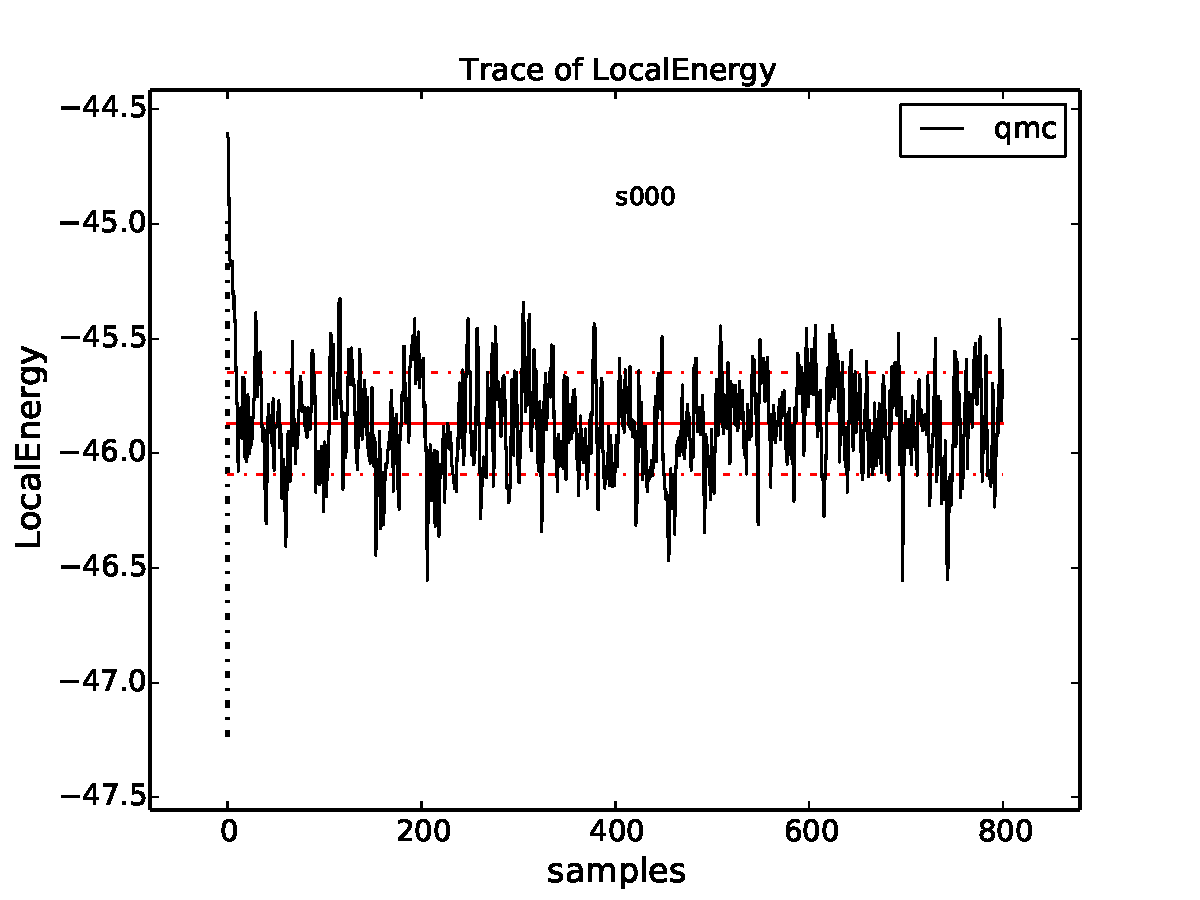
\includegraphics[trim = 0mm 0mm 0mm 0mm, clip,width=0.75\columnwidth]{figures/qmca_mean_error_trace.pdf}
\end{center}
\caption{Trace of the VMC local energy for an 8 atom cell of diamond generated with \texttt{qmca}.  The x-axis (``samples'') refers to the VMC block index in this case.
\label{fig:qmca_mean_error_trace}
}
\end{figure}

If we exclude none of the equilibration data points, we get an 
erroneous estimate of $-45.870(2)$ Ha for the local energy:
\begin{shade}
>qmca -q e -e 0 qmc.s000.scalar.dat 
qmc  series 0  LocalEnergy           =  -45.870071 +/- 0.018072
\end{shade}
\noindent
The equilibration period is typically estimated by eye, though one should
check a few conservative values to ensure that the mean remains 
unaffected.  In this dataset, the equilibration appears to have been 
reached after 100 samples or so.  After excluding the first 100 
VMC blocks from the analysis we get:
\begin{shade}
>qmca -q e -e 100 qmc.s000.scalar.dat 
qmc  series 0  LocalEnergy           =  -45.877363 +/- 0.017432
\end{shade}
\noindent
This estimate ($-45.877(2)$ Ha) differs significantly from the 
$-45.870(2)$ Ha figure obtained from the full set of data, but it 
agrees with the rough estimate of $-45.876(2)$ Hartrees obtained 
with the abbreviated command (``\texttt{qmca -q e qmc.s000.scalar.dat}'').
This is because \texttt{qmca} makes a heuristic guess at the 
equilibration period and got it reasonably correct in this case. 
There are many cases where the heuristic guess fails and it should not 
be relied on for quality results.

We have so far obtained a statistically correct mean.  To obtain 
a statistically correct error bar it is best to include $\sim$100 or more 
statistically independent samples.  An estimate of the number 
of independent samples can be obtained by considering the 
autocorrelation time, which is essentially a measure of the number of 
samples that must be traversed before an uncorrelated/independent sample 
is reached.  We can get an estimate of the autocorrelation time 
in the following way:
\begin{shade}
>qmca -q e -e 100 qmc.s000.scalar.dat --sac
qmc  series 0  LocalEnergy           =  -45.877363 +/- 0.017432    4.8 
\end{shade}
\noindent
The flag ``\texttt{--sac}'' stands for (s)how (a)uto(c)orrelation.  
In this case the autocorrelation estimate is $4.8\approx 5$ samples. 
Since the total run contained 800 samples and we have excluded 100 of 
them, we can estimate the number of independent samples as 
$(800-100)/5=140$.  In this case, the error bar is expected to be 
estimated reasonably well.

Please keep in mind that the error bar represents the expected range
of the mean with a certainty of only $\sim 70\%$, i.e. it is a one
sigma error bar.  The actual mean value will lie outside the range
indicated by the error bar in one out of every three runs and in a set
of 20 runs one value can be expected to deviate from its estimate by
twice the error bar.


\subsection{Judging wavefunction optimization}
\label{sec:qmca_judge_opt}
Wavefunction optimization is a highly non-linear and sometimes 
sensitive process.  As such, there is a risk that systematic 
errors encountered at this stage of the QMC process can be propagated 
into subsequent (expensive) DMC runs unless they are guarded against 
with vigilance.

In this section we again consider an 8 atom cell of diamond, but 
now in the context of Jastrow optimization (one- and two-body terms). 
In optimization runs it is often preferable to use a large number 
of \texttt{warmupsteps} ($\sim 100$) so that equilibration bias does 
not propagate into the optimization process.  We can check that 
the added warmup has had its intended effect by again checking the 
local energy trace:
\begin{shade}
>qmca -t -q e *scalar*
\end{shade}
\noindent
The resulting plot can be found in Fig. \ref{fig:qmca_judge_opt}. 
In this case sufficient \texttt{warmupsteps} were used to exit 
the equilibration period before samples were collected and we can 
proceed without using the ``\texttt{-e}'' option with \texttt{qmca}.

\begin{figure}
\begin{center}
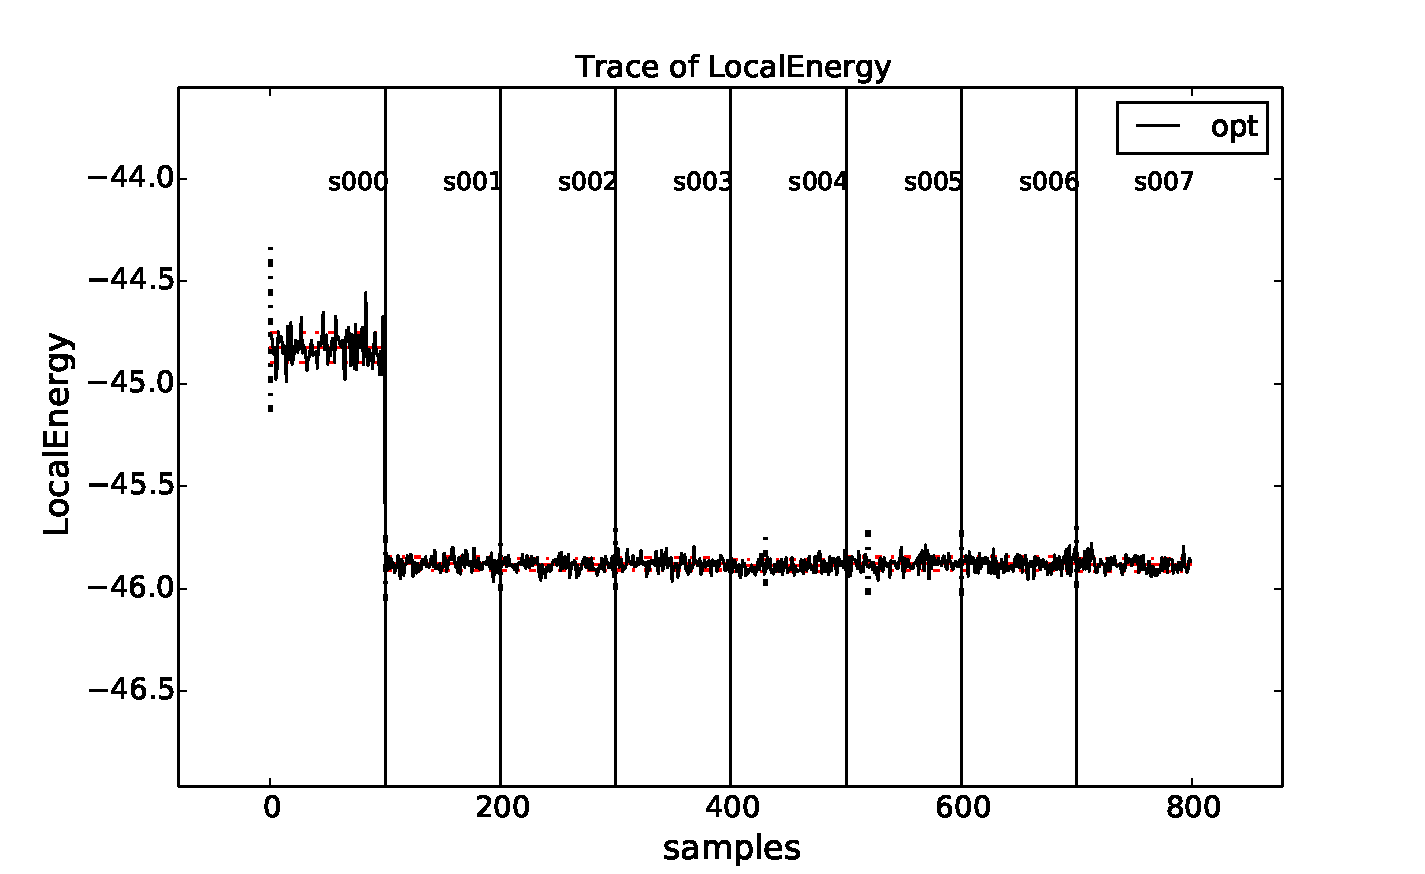
\includegraphics[trim = 0mm 0mm 0mm 0mm, clip,width=0.9\columnwidth]{figures/qmca_judge_opt.pdf}
\end{center}
\caption{Trace of the local energy during one- and two-body Jastrow optimization for an 8 atom cell of diamond generated with \texttt{qmca}.  Data for each optimization cycle (QMCPACK series) is separated by a vertical black line.
\label{fig:qmca_judge_opt}
}
\end{figure}

After inspecting the trace, we should inspect the text output 
from \texttt{qmca}, now including the total energy and its variance:
\begin{shade}
>qmca -q ev opt*scalar.dat
                            LocalEnergy               Variance           ratio 
opt  series 0  -44.823616 +/- 0.007430   7.054219 +/- 0.041998   0.1574 
opt  series 1  -45.877643 +/- 0.003329   1.095362 +/- 0.041154   0.0239 
opt  series 2  -45.883191 +/- 0.004149   1.077942 +/- 0.021555   0.0235 
opt  series 3  -45.877524 +/- 0.003094   1.074047 +/- 0.010491   0.0234 
opt  series 4  -45.886062 +/- 0.003750   1.061707 +/- 0.014459   0.0231 
opt  series 5  -45.877668 +/- 0.003475   1.091585 +/- 0.021637   0.0238 
opt  series 6  -45.877109 +/- 0.003586   1.069205 +/- 0.009387   0.0233 
opt  series 7  -45.882563 +/- 0.004324   1.058771 +/- 0.008651   0.0231 
\end{shade}
\noindent
The flags ``\texttt{-q ev}'' requested the energy (\texttt{e}) and 
the variance (\texttt{v}).  For this combination of quantities, a 
third column (``\texttt{ratio}'') is printed containing the ratio 
of the variance and the absolute value of the local energy.
The variance/energy ratio is an intensive quantity and is useful  
to inspect regardless of the system under study.  Successful 
optimization of molecules and solids of any size generally result 
in comparable values for the variance/energy ratio. 

The first line of 
the output (``\texttt{series 0}'') corresponds to the local energy 
and variance of the system without a Jastrow factor (all Jastrow 
coefficients were initialized to zero in this case), reflecting the 
quality of the orbitals alone. For pseudopotential systems, a 
variance/energy ratio $>0.20$ Ha generally indicates there is a problem 
with the input orbitals that needs to be resolved prior to 
performing wavefunction optimization.  

The subsequent lines correspond to energies and variances of 
intermediate parameterizations of the trial wavefunction during 
the optimization process.  The output line containing 
``\texttt{opt  series 1}'', for example, corresponds to the trial 
wavefunction parameterized during the ``\texttt{series 0}'' step 
(the parameters of this wavefunction would be found in an output 
file matching \texttt{*s000*opt.xml}).  The first thing to check 
about the resulting optimization is again the variance/energy ratio. 
For pseudopotential systems, a variance/energy ratio $<0.03$ Ha is 
consistent with a trial wavefunction of production quality, and values 
of $0.01$ Ha are rarely obtainable for standard Slater-Jastrow 
wavefunctions.  By this metric, all parameterizations obtained for 
optimizations performed in series 0-6 are of comparable quality 
(note that the quality of the wavefunction obtained during optimization 
series 7 is effectively unknown).

A good way to further discriminate among the parameterizations is to 
plot the energy and variance as a function of series with \texttt{qmca}:
\begin{shade}
>qmca -p -q ev opt*scalar.dat
\end{shade}
\noindent
The ``\texttt{-p}'' option results in plots of means plus error bars 
vs. series for all requested quantities.
The resulting plots for the local energy and variance are shown 
in Fig. \ref{fig:qmca_opt_ev}.  In this case the resulting energies 
and variances are statistically indistinguishable for all optimization 
cycles.  

\begin{figure}
  \centering
  \begin{subfigure}[t]{0.47\textwidth}
    \centering
    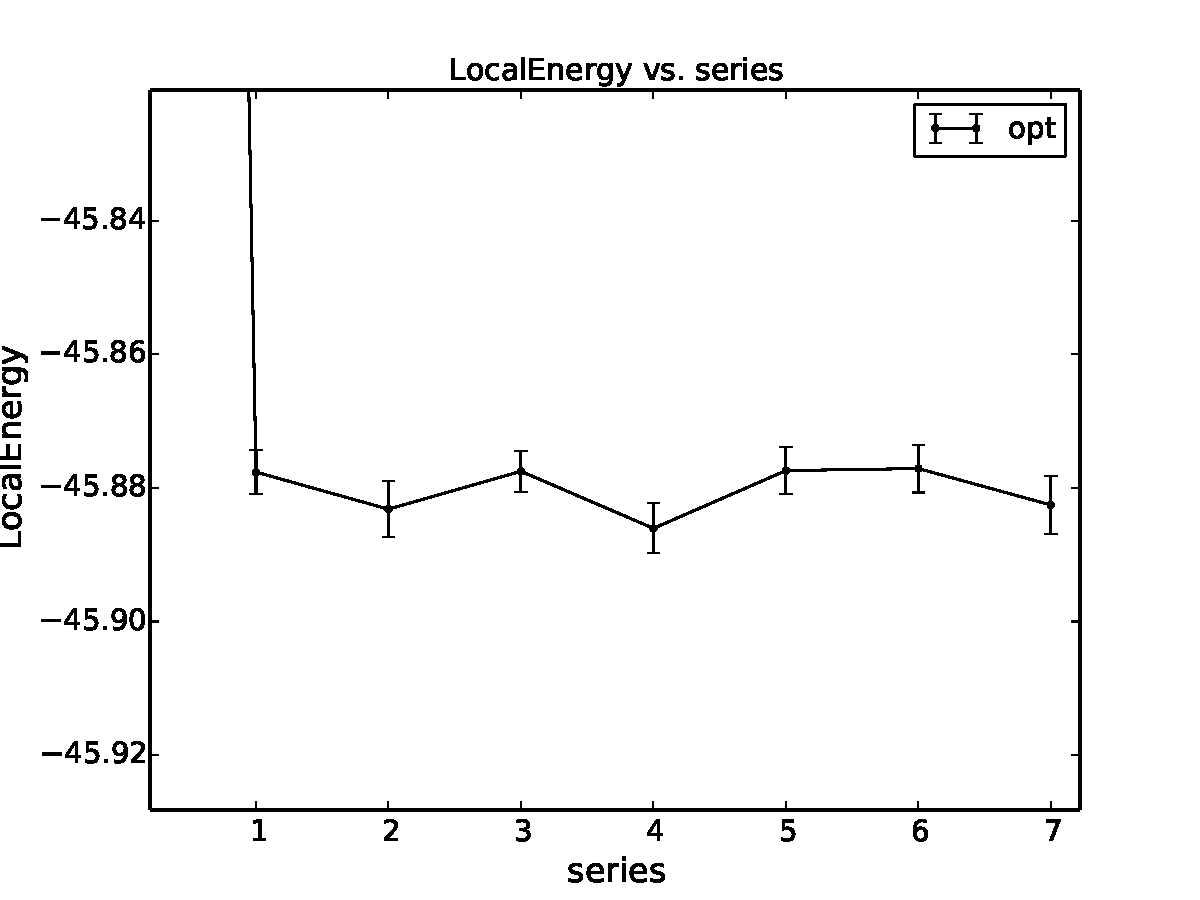
\includegraphics[trim=0mm 0mm 4mm 0mm,clip,width=\linewidth]{figures/qmca_opt_energy.pdf}
  \end{subfigure}
  \begin{subfigure}[t]{0.47\textwidth}
    \centering
    \includegraphics[trim=2mm 0mm 4mm 0mm,clip,width=\linewidth]{figures/qmca_opt_variance.pdf}
  \end{subfigure}
  \caption{Energy and variance vs. optimization series for an 8 atom cell of diamond as plotted by \texttt{qmca}.\label{fig:qmca_opt_ev}}
\end{figure}

A good way to choose the optimal wavefunction for use in DMC is to select 
the one with lowest statistically significant energy within the set of 
optimized wavefunctions with reasonable variance (\emph{e.g.} among 
those with variance/energy ratio $<0.03$ Ha).  For pseudopotential 
calculations, minimizing according to the total energy is recommended 
to reduce locality errors in DMC.


\subsection{Judging diffusion Monte Carlo runs}
\label{sec:qmca_judge_dmc}
Judging the quality of the DMC projection process requires more 
care than this needed in VMC.  In order to reduce bias, a small 
timestep is required in the approximate projector but this also 
leads to slow equilibration and long autocorrelation times.  
Systematic errors in the projection process can also arise from 
statistical fluctuations due to pseudopotentials or from trial 
wavefunctions with larger than necessary variance.

\begin{figure}
\begin{center}
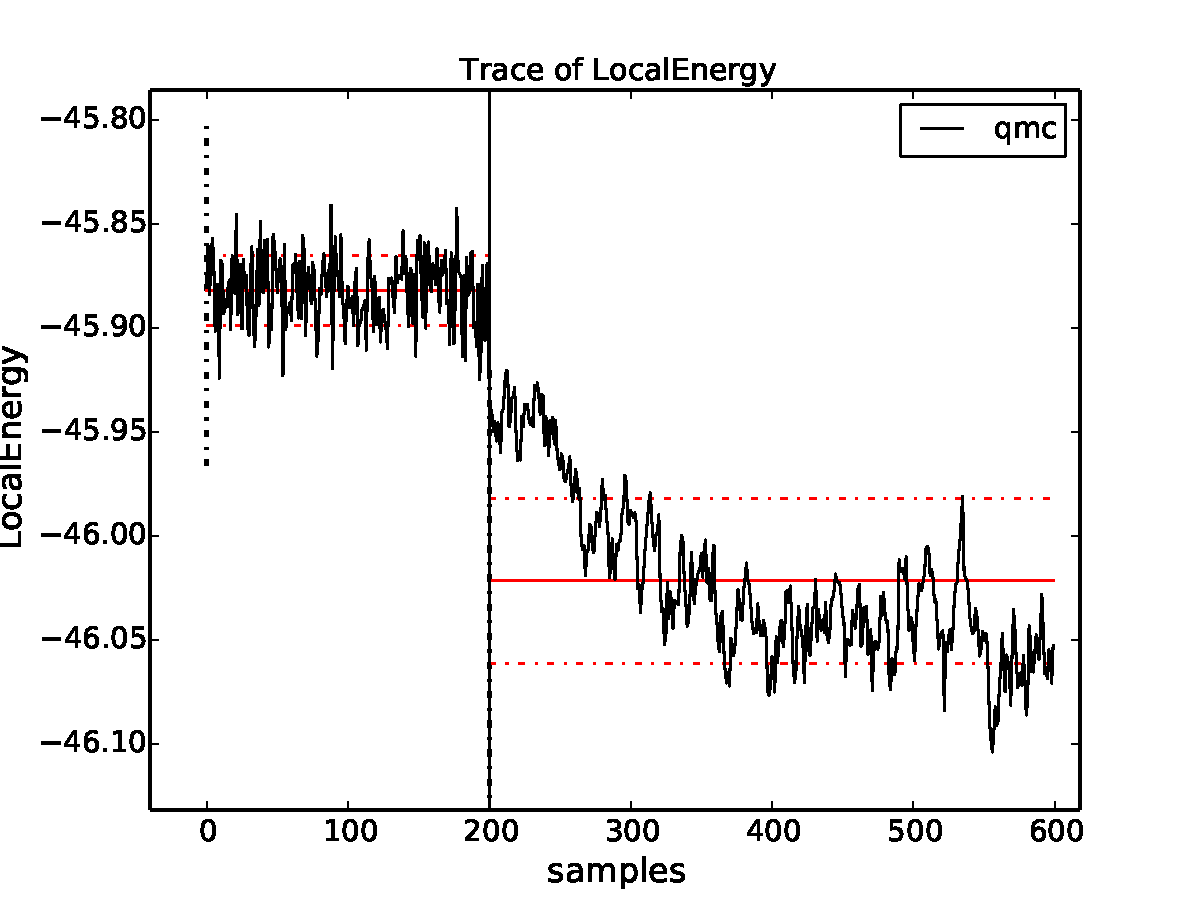
\includegraphics[trim = 0mm 0mm 0mm 0mm, clip,width=0.75\columnwidth]{figures/qmca_short_dmc.pdf}
\end{center}
\caption{Trace of the local energy for VMC followed by DMC with a small timestep ($0.002$ Ha$^{-1}$) for an 8 atom cell of diamond generated with \texttt{qmca}.  
\label{fig:qmca_short_dmc}
}
\end{figure}

To illustrate the problems that can arise with respect to slow 
equilibration and long autocorrelation times, we consider the 
8 atom diamond system with VMC ($200$ blocks of $160$ steps) followed 
by DMC ($400$ blocks of $5$ steps) with a small timestep ($0.002$ Ha$^{-1}$).
A good first step in assessing the quality of any DMC run is 
to plot the trace of the local energy:
\begin{shade}
>qmca -t -q e -e 0 *scalar*
\end{shade}
\noindent
The resulting trace plot is shown in Fig. \ref{fig:qmca_short_dmc}.  
As always, the DMC local energy decreases exponentially away from 
the VMC value but in this case it takes a long time to do so.  
At least half of the DMC run is inefficiently consumed by equilibration.
If we are not careful to inspect and remove the transient, the estimated 
DMC energy will be strongly biased by the transient as shown by the 
horizontal red line (estimated mean) in the figure.  The autocorrelation 
time is also large ($\sim 12$ blocks):
\begin{shade}
>qmca -q e -e 200 --sac *s001.scalar*
qmc  series 1  LocalEnergy           =  -46.045720 +/- 0.004813   11.6
\end{shade}
\noindent
Of the included 200 blocks, fewer than 20 contribute to the estimated error 
bar, indicating that we cannot trust the reported error bar.  
This can also be demonstrated directly from the data.  If we halve the number 
of samples included to 100, we would expect from Gaussian statistics 
that the error bar would grow by a factor of $\sqrt{2}$, but instead we 
get
\begin{shade}
>qmca -q e -e 300 *s001.scalar*
qmc  series 1  LocalEnergy           =  -46.048537 +/- 0.009280
\end{shade}
\noindent
which erroneously shows an estimated increase in the error bar by a factor 
of about two.  Overall this run is simply too short to gain meaningful 
information.  

Consider the case where we are interested in the cohesive energy of 
diamond and, after having performed a timestep study of the cohesive 
energy, we have found that the energy difference between bulk diamond 
and atomic carbon converges to our required accuracy with a larger 
timestep of $0.01$ Ha$^{-1}$.  In a production setting, a small cell 
could be used to determine  the appropriate timestep while a larger 
cell would subsequently be used to obtain a converged cohesive energy, 
though for purposes of demonstration we still proceed with the 8 atom 
cell here.  The new timestep of $0.01$ Ha$^{-1}$ will result in a shorter 
autocorrelation time than the smaller timestep used previously, but 
we would like to shorten the equilibration time further still.  This 
can be achieved by using a larger timestep (say $0.02$ Ha$^{-1}$) in a 
short intermediate DMC run used to walk down the transient.  The 
rapidly achieved equilibrium with the $0.02$ Ha$^{-1}$ timestep 
projector will be much nearer to the $0.01$ Ha$^{-1}$ timestep one 
we seek than the original VMC equilibrium, and so we can expect 
a shortened secondary equilibration time in the production 
$0.01$ Ha$^{-1}$ timestep run. Note that this procedure is fully 
general, even if one has to deal with an even shorter 
timestep--\emph{e.g.} $0.002$ Ha$^{-1}$--for a particular problem.

\begin{figure}
\begin{center}
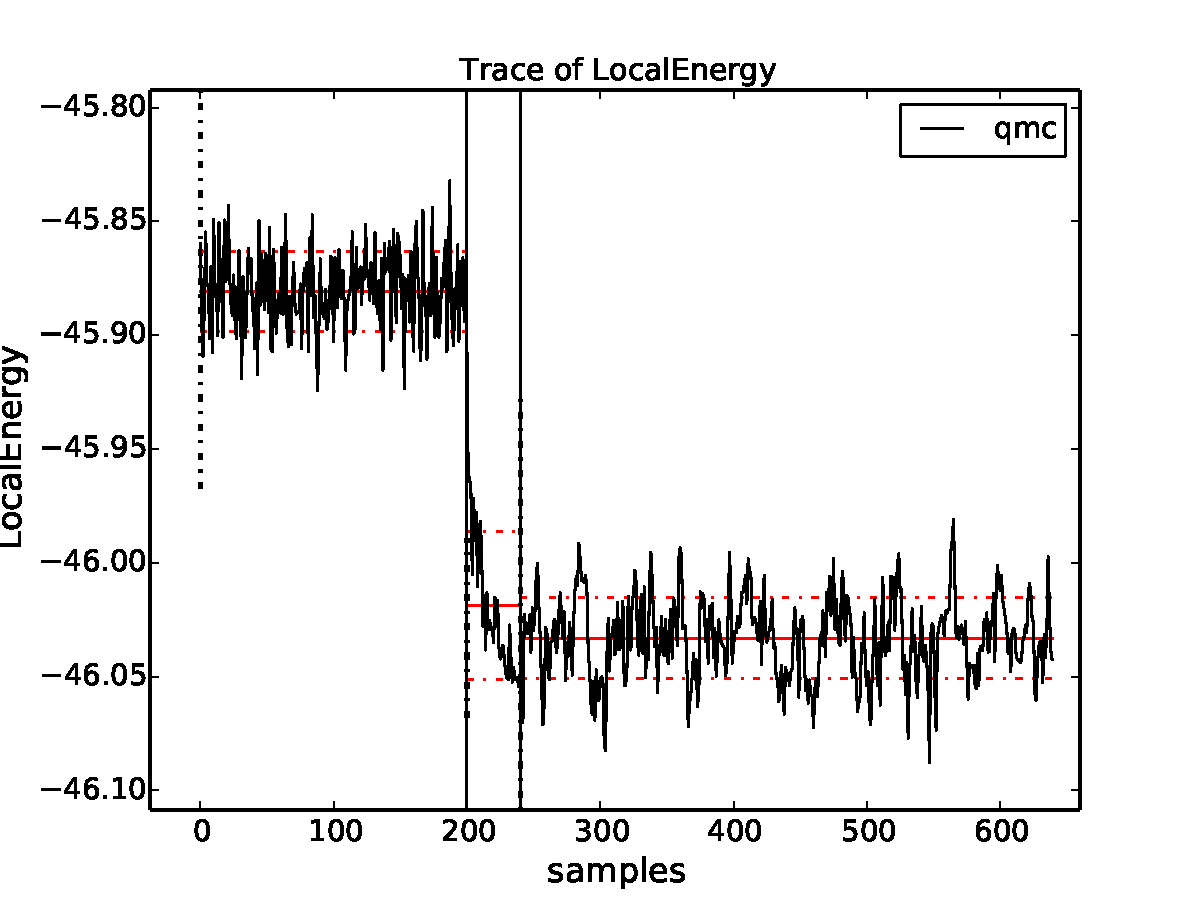
\includegraphics[trim = 0mm 0mm 0mm 0mm, clip,width=0.75\columnwidth]{figures/qmca_accel_dmc.pdf}
\end{center}
\caption{Trace of the local energy for VMC followed by a short intermediate DMC with a large timestep ($0.02$ Ha$^{-1}$) and finally a production DMC run with a timestep of $0.01$ Ha$^{-1}$.  Calculations were performed in an 8 atom cell of diamond.  
\label{fig:qmca_accel_dmc}
}
\end{figure}

We now rerun the prior example but with an intermediate DMC 
calculation using $40$ blocks of $5$ steps with a timestep of 
$0.02$ Ha$^{-1}$ followed by a production DMC calculation 
using $400$ blocks of $10$ steps with a timestep of $0.01$ Ha$^{-1}$.
We again plot the local energy trace using \texttt{qmca}
\begin{shade}
>qmca -t -q e -e 0 *scalar*
\end{shade}
\noindent
with the result shown in Fig. \ref{fig:qmca_accel_dmc}.
The projection transient has been effectively contained in the 
short DMC run with a larger timestep.  As expected, the 
production run contains only a short equilibration period.
Removing the first 20 blocks as a precaution, we obtain an estimate 
of the total energy in VMC and DMC:
\begin{shade}
>qmca -q ev -e 20 --sac qmc.*.scalar.dat 
                            LocalEnergy               Variance           ratio 
qmc  series 0  -45.881042 +/- 0.001283    1.0   1.076726 +/- 0.007013    1.0   0.0235 
qmc  series 1  -46.040814 +/- 0.005046    3.9   1.011303 +/- 0.016807    1.1   0.0220 
qmc  series 2  -46.032960 +/- 0.002077    5.2   1.014940 +/- 0.002547    1.0   0.0220 
\end{shade}
\noindent
Notice that the variance energy ratio in DMC ($0.220$ Ha) is similar to, but 
slightly smaller than, what is obtained with VMC ($0.235$ Ha).  If the DMC 
variance/energy ratio is ever significantly larger than in VMC, this is 
cause to be concerned about the correctness of the DMC run.  Also notice 
the estimated autocorrelation time ($\sim 5$ blocks).  This leaves us with 
an estimated $\sim 76$ independent samples, though we should recall that 
the autocorrelation time is also a statistical estimate which can be improved 
with more data.  We can gain a better estimate of the autocorrelation 
time by using the \texttt{*.dmc.dat} files which contain output data resolved 
per step rather than per block (there are $10\times$ more steps than blocks 
in this example case):
\begin{shade}
>qmca -q ev -e 200 --sac qmc.s002.dmc.dat 
                            LocalEnergy               Variance           ratio 
qmc  series 2  -46.032909 +/- 0.002068   31.2   1.015781 +/- 0.002536    1.4   0.0221 
\end{shade}
\noindent
This results in an estimated autocorrelation time of $\sim 31$ steps, or 
$\sim 3$ blocks, indicating that we actually have $\sim 122$ independent 
samples which should be sufficient to obtain a trustworthy error bar.
Our final DMC total energy is estimated to be $-46.0329(2)$ Ha.

\begin{figure}
\begin{center}
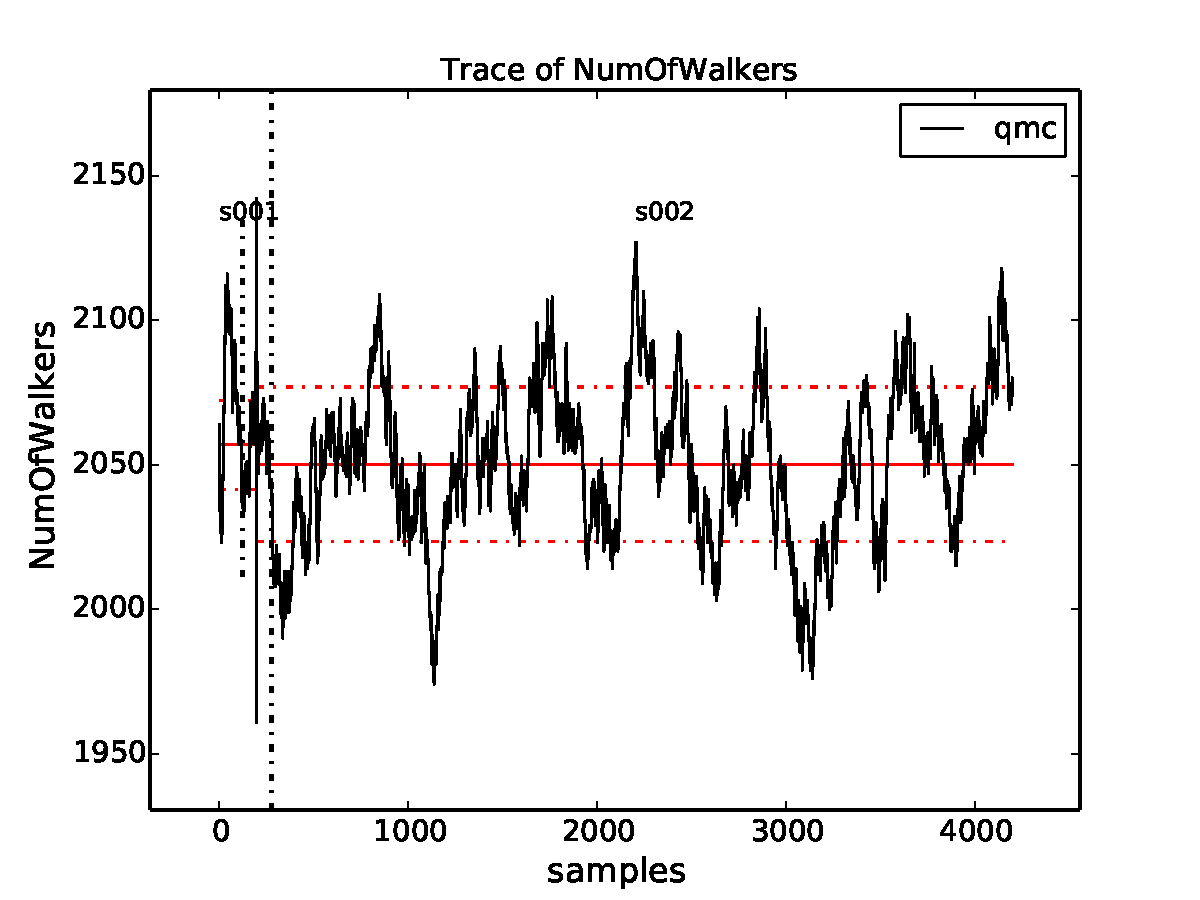
\includegraphics[trim = 0mm 0mm 0mm 0mm, clip,width=0.75\columnwidth]{figures/qmca_pop_trace.pdf}
\end{center}
\caption{Trace of the DMC walker population for an 8 atom cell of diamond obtained with \texttt{qmca}.  
\label{fig:qmca_pop_trace}
}
\end{figure}

Another simulation property that should be explicitly monitored  
is the behavior of the DMC walker population.  Data regarding the 
walker population is contained in the \texttt{*.dmc.dat} files.
In Fig. \ref{fig:qmca_pop_trace} we show the trace of the DMC 
walker population for the current run:
\begin{shade}
>qmca -t -q nw *dmc.dat
qmc  series 1  NumOfWalkers          =  2056.905405 +/- 8.775527 
qmc  series 2  NumOfWalkers          =  2050.164160 +/- 4.954850 
\end{shade}
\noindent
Following a DMC run the walker population should be checked for 
two qualities: 1) that the population is sufficiently large (a number 
$>2000$ is generally sufficient to reduce population control bias) and  
2) that the population fluctuates benignly around its intended target 
value. In this case the target walker count (provided in the input file)
was $2048$ and we can confirm from the plot that the population is simply 
fluctuating around this value.  Also from the text output we have a dynamic 
population estimate of 2050(5) walkers.  Rapid population reductions or 
increases--population explosions--are indicative of problems with a run.  
These issues sometimes result from using a considerably poor wavefunction 
(see comments regarding variance/energy ratio above and in the preceding 
subsections).  QMCPACK has internal guards in place that prevent 
the population from exceeding certain maximum and minimum bounds, so 
in particularly faulty runs one might see the population ``stabilize'' 
to a constant value much larger or smaller than the target.  In these 
cases the cause(s) for the divergent population behavior need to 
be investigated and resolved before proceeding further.



\subsection{Obtaining other quantities}
\label{sec:qmca_other_quantities}
A number of other scalar valued quantities are available with 
\texttt{qmca}.  To obtain text output for all quantities 
available, simply exclude the ``\texttt{-q}'' option used in 
the prior examples.  Below is example output for a DMC calculation 
of the 8 atom diamond system from the \texttt{scalar.dat} file:
\begin{shade}
>qmca -e 20 qmc.s002.scalar.dat 
qmc  series 2 
  LocalEnergy           =          -46.0330 +/-           0.0021 
  Variance              =            1.0149 +/-           0.0025 
  Kinetic               =            33.851 +/-            0.019 
  LocalPotential        =           -79.884 +/-            0.020 
  ElecElec              =          -11.4483 +/-           0.0083 
  LocalECP              =           -22.615 +/-            0.029 
  NonLocalECP           =            5.2815 +/-           0.0079 
  IonIon                =            -51.10 +/-             0.00 
  LocalEnergy_sq        =           2120.05 +/-             0.19 
  BlockWeight           =          20514.27 +/-            48.38 
  BlockCPU              =            1.4890 +/-           0.0038 
  AcceptRatio           =         0.9963954 +/-        0.0000055 
  Efficiency            =             71.88 +/-             0.00 
  TotalTime             =            565.80 +/-             0.00 
  TotalSamples          =           7795421 +/-                0 
\end{shade}
\noindent
Similarly, for the \texttt{dmc.dat} file we get
\begin{shade}
>qmca -e 20 qmc.s002.dmc.dat 
qmc  series 2 
  LocalEnergy           =          -46.0329 +/-           0.0020 
  Variance              =            1.0162 +/-           0.0025 
  TotalSamples          =           8201275 +/-                0 
  TrialEnergy           =          -46.0343 +/-           0.0023 
  DiffEff               =         0.9939150 +/-        0.0000088 
  Weight                =           2050.23 +/-             4.82 
  NumOfWalkers          =              2050 +/-                5 
  LivingFraction        =          0.996427 +/-         0.000021 
  AvgSentWalkers        =            0.2625 +/-           0.0011 
\end{shade}

Any subset of desired quantities can be obtained by using the 
``\texttt{-q}'' option with either the full names of the quantities 
listed above 
\begin{shade}
>qmca -q 'LocalEnergy Kinetic LocalPotential' -e 20 qmc.s002.scalar.dat 
qmc  series 2 
  LocalEnergy           =          -46.0330 +/-           0.0021 
  Kinetic               =            33.851 +/-            0.019 
  LocalPotential        =           -79.884 +/-            0.020 
\end{shade}
\noindent
or with their corresponding abbreviations
\begin{shade}
>qmca -q ekp -e 20 qmc.s002.scalar.dat 
qmc  series 2 
  LocalEnergy           =          -46.0330 +/-           0.0021 
  Kinetic               =            33.851 +/-            0.019 
  LocalPotential        =           -79.884 +/-            0.020 
\end{shade}
\noindent
Abbreviations for each quantity can be found by typing \texttt{qmca}
at the command line with no other input.  A current list is provided 
below:
\begin{shade}
  Abbreviations and full names for quantities:
    ar              = AcceptRatio
    bc              = BlockCPU
    bw              = BlockWeight
    ce              = CorrectedEnergy
    de              = DiffEff
    e               = LocalEnergy
    ee              = ElecElec
    eff             = Efficiency
    ii              = IonIon
    k               = Kinetic
    kc              = KEcorr
    l               = LocalECP
    le2             = LocalEnergy_sq
    mpc             = MPC
    n               = NonLocalECP
    nw              = NumOfWalkers
    p               = LocalPotential
    sw              = AvgSentWalkers
    te              = TrialEnergy
    ts              = TotalSamples
    tt              = TotalTime
    v               = Variance
    w               = Weight
\end{shade}
\noindent
Please see the output overview for \texttt{scalar.dat} 
(Sec. \ref{sec:scalardat_file}) and \texttt{dmc.dat} 
(Sec. \ref{sec:dmc_file}) for more information about 
these quantities.  The data analysis aspects for these 
quantities is essentially the same as for the local 
energy as covered in the preceding subsections. 
Quantities that do not belong to an equilibrium distribution 
(\emph{e.g.} \texttt{BlockCPU}) are somewhat different, though they 
still exhibit statistical fluctuations.


\subsection{Processing multiple files}
\label{sec:qmca_multiple_files}
Batch file processing is a common use case for \texttt{qmca}. 
If we consider an ``equation of state'' calculation involving 
the 8 atom diamond cell we have used so far, we might be interested 
in the total energy for the various supercell volumes along the 
trajectory from compression to expansion.  After checking 
the traces (``\texttt{qmca -t -q e scale\_*/vmc/*scalar*}'') 
to settle on a sensible equilibration cutoff as discussed in 
the preceding subsections we can obtain the total energies 
all at once:
\begin{shade}
>qmca -q ev -e 40 scale_*/vmc/*scalar*
                            LocalEnergy               Variance           ratio 
scale_0.80/vmc/qmc  series 0 -44.670984 +/- 0.006051  2.542384 +/- 0.019902  0.0569 
scale_0.82/vmc/qmc  series 0 -44.982818 +/- 0.005757  2.413011 +/- 0.022626  0.0536 
scale_0.84/vmc/qmc  series 0 -45.228257 +/- 0.005374  2.258577 +/- 0.019322  0.0499 
scale_0.86/vmc/qmc  series 0 -45.415842 +/- 0.005532  2.204980 +/- 0.052978  0.0486 
scale_0.88/vmc/qmc  series 0 -45.570215 +/- 0.004651  2.061374 +/- 0.014359  0.0452 
scale_0.90/vmc/qmc  series 0 -45.683684 +/- 0.005009  1.988539 +/- 0.018267  0.0435 
scale_0.92/vmc/qmc  series 0 -45.751359 +/- 0.004928  1.913282 +/- 0.013998  0.0418 
scale_0.94/vmc/qmc  series 0 -45.791622 +/- 0.005026  1.843704 +/- 0.014460  0.0403 
scale_0.96/vmc/qmc  series 0 -45.809256 +/- 0.005053  1.829103 +/- 0.014536  0.0399 
scale_0.98/vmc/qmc  series 0 -45.806235 +/- 0.004963  1.775391 +/- 0.015199  0.0388 
scale_1.00/vmc/qmc  series 0 -45.783481 +/- 0.005293  1.726869 +/- 0.012001  0.0377 
scale_1.02/vmc/qmc  series 0 -45.741655 +/- 0.005627  1.681776 +/- 0.011496  0.0368 
scale_1.04/vmc/qmc  series 0 -45.685101 +/- 0.005353  1.682608 +/- 0.015423  0.0368 
scale_1.06/vmc/qmc  series 0 -45.615164 +/- 0.005978  1.652155 +/- 0.010945  0.0362 
scale_1.08/vmc/qmc  series 0 -45.543037 +/- 0.005191  1.646375 +/- 0.013446  0.0361 
scale_1.10/vmc/qmc  series 0 -45.450976 +/- 0.004794  1.707649 +/- 0.048186  0.0376 
scale_1.12/vmc/qmc  series 0 -45.371851 +/- 0.005103  1.686997 +/- 0.035920  0.0372 
scale_1.14/vmc/qmc  series 0 -45.265490 +/- 0.005311  1.631614 +/- 0.012381  0.0360 
scale_1.16/vmc/qmc  series 0 -45.161961 +/- 0.004868  1.656586 +/- 0.014788  0.0367 
scale_1.18/vmc/qmc  series 0 -45.062579 +/- 0.005971  1.671998 +/- 0.019942  0.0371 
scale_1.20/vmc/qmc  series 0 -44.960477 +/- 0.004888  1.651864 +/- 0.009756  0.0367 
\end{shade}
\noindent

In this case, we are using a Jastrow factor optimized only at the 
equilibrium geometry (``\texttt{scale\_1.00}'') but with radial 
cutoffs restricted to the Wigner-Seitz radius of the most compressed 
supercell (``\texttt{scale\_0.80}'') to avoid introducing wavefunction 
cusps at the cell boundary (QMCPACK would have aborted with a warning in 
this case, had we tried).  It is clear that this restricted Jastrow factor 
is not an optimal choice as it yields variance/energy ratios between $0.036$ 
and $0.057$ Ha.  This issue is largely a result of our undersized (8 atom) 
supercell and larger cells should always be used in real production 
calculations.

Batch processing is also possible for multiple quantities.  If multiple 
quantities are requested, an additional line is inserted to separate 
results from different runs:
\begin{shade}
>qmca -q 'e bc eff' -e 40 scale_*/vmc/*scalar*
scale_0.80/vmc/qmc  series 0 
  LocalEnergy           =          -44.6710 +/-           0.0061 
  BlockCPU              =           0.02986 +/-          0.00038 
  Efficiency            =          38104.00 +/-             0.00 

scale_0.82/vmc/qmc  series 0 
  LocalEnergy           =          -44.9828 +/-           0.0058 
  BlockCPU              =           0.02826 +/-          0.00013 
  Efficiency            =          44483.91 +/-             0.00 

scale_0.84/vmc/qmc  series 0 
  LocalEnergy           =          -45.2283 +/-           0.0054 
  BlockCPU              =           0.02747 +/-          0.00030 
  Efficiency            =          52525.12 +/-             0.00 

scale_0.86/vmc/qmc  series 0 
  LocalEnergy           =          -45.4158 +/-           0.0055 
  BlockCPU              =           0.02679 +/-          0.00013 
  Efficiency            =          50811.55 +/-             0.00 

scale_0.88/vmc/qmc  series 0 
  LocalEnergy           =          -45.5702 +/-           0.0047 
  BlockCPU              =           0.02598 +/-          0.00015 
  Efficiency            =          74148.79 +/-             0.00 

scale_0.90/vmc/qmc  series 0 
  LocalEnergy           =          -45.6837 +/-           0.0050 
  BlockCPU              =           0.02527 +/-          0.00011 
  Efficiency            =          65714.98 +/-             0.00 

...
\end{shade}



\subsection{Twist averaging}
\label{sec:qmca_twist_average}
Twist averaging can be performed straightforwardly for any 
output quantity listed in Sec. \ref{sec:qmca_other_quantities} 
with \texttt{qmca}.  We illustrate these capabilities by 
repeating the 8 atom diamond DMC runs performed in Sec. 
\ref{sec:qmca_judge_dmc} at eight real valued supercell twist 
angles (a $2\times 2\times 2$ Monkhorst-Pack grid centered at 
the $\Gamma$-point).  Data traces for each twist can be overlapped 
on the same plot:
\begin{shade}
>qmca -to -q e -e '30 20 30' *scalar* --legend outside
\end{shade}
\noindent
The ``\texttt{-o}'' option requests the plots be overlapped; 
eight separate plots would be generated otherwise.  The 
equilibration input ``\texttt{-e '30 20 30'}'' cuts out from 
the analyzed data the first 30 blocks for series 0 (VMC), 
20 blocks for series 1 (intermediate DMC), and 30 blocks for 
series 2 (production DMC).  The resulting plot is shown in 
Fig. \ref{fig:qmca_twist_overlap}

\begin{figure}
\begin{center}
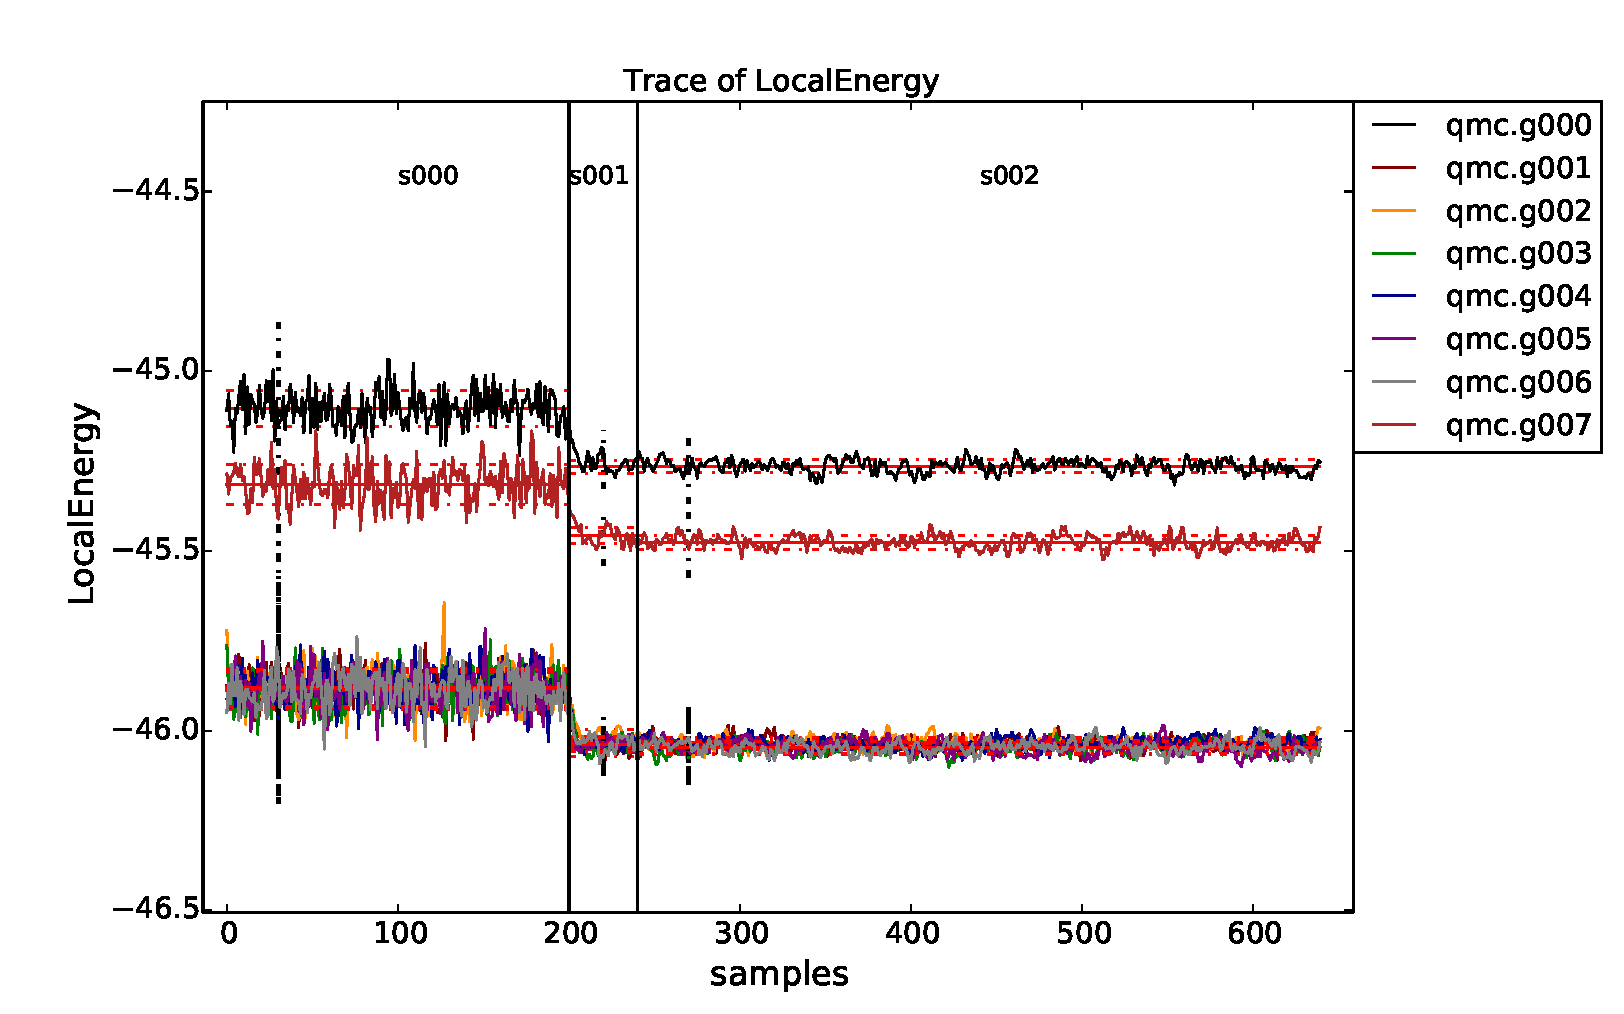
\includegraphics[trim = 0mm 0mm 0mm 0mm, clip,width=0.9\columnwidth]{figures/qmca_twist_trace_overlap.pdf}
\end{center}
\caption{Overlapped energy traces from VMC to DMC for an 8 supercell of diamond obtained with \texttt{qmca}.  Data for each twist appears in a different color.
\label{fig:qmca_twist_overlap}
}
\end{figure}

Twist averaging is performed by providing the ``\texttt{-a}'' 
option.  If provided on its own, uniform weights are applied 
to each twist angle.  To obtain a trace plot with twist averaging 
enforced, use a command similar to the following:
\begin{shade}
>qmca -a -t -q e -e '30 20 30' *scalar*
\end{shade}
\noindent
The resulting plot is shown in Fig. \ref{fig:qmca_twist_average}.
As can be seen from the trace plot, the chosen equilibration lengths 
are appropriate and we proceed to obtain the twist averaged total energy
from the \texttt{scalar.dat} files
\begin{shade}
>qmca -a -q ev -e 30 --sac *s002.scalar*
                            LocalEnergy               Variance           ratio 
avg  series 2  -45.873369 +/- 0.000753    5.3   1.028751 +/- 0.001056    1.3   0.0224 
\end{shade}
\noindent
and also from the \texttt{dmc.dat} files
\begin{shade}
>qmca -a -q ev -e 300 --sac *s002.dmc*
                            LocalEnergy               Variance           ratio 
avg  series 2  -45.873371 +/- 0.000741   30.5   1.028843 +/- 0.000972    1.6   0.0224 
\end{shade}
\noindent
yielding a twist averaged total energy of $-45.8733(8)$ Ha. 

\begin{figure}
\begin{center}
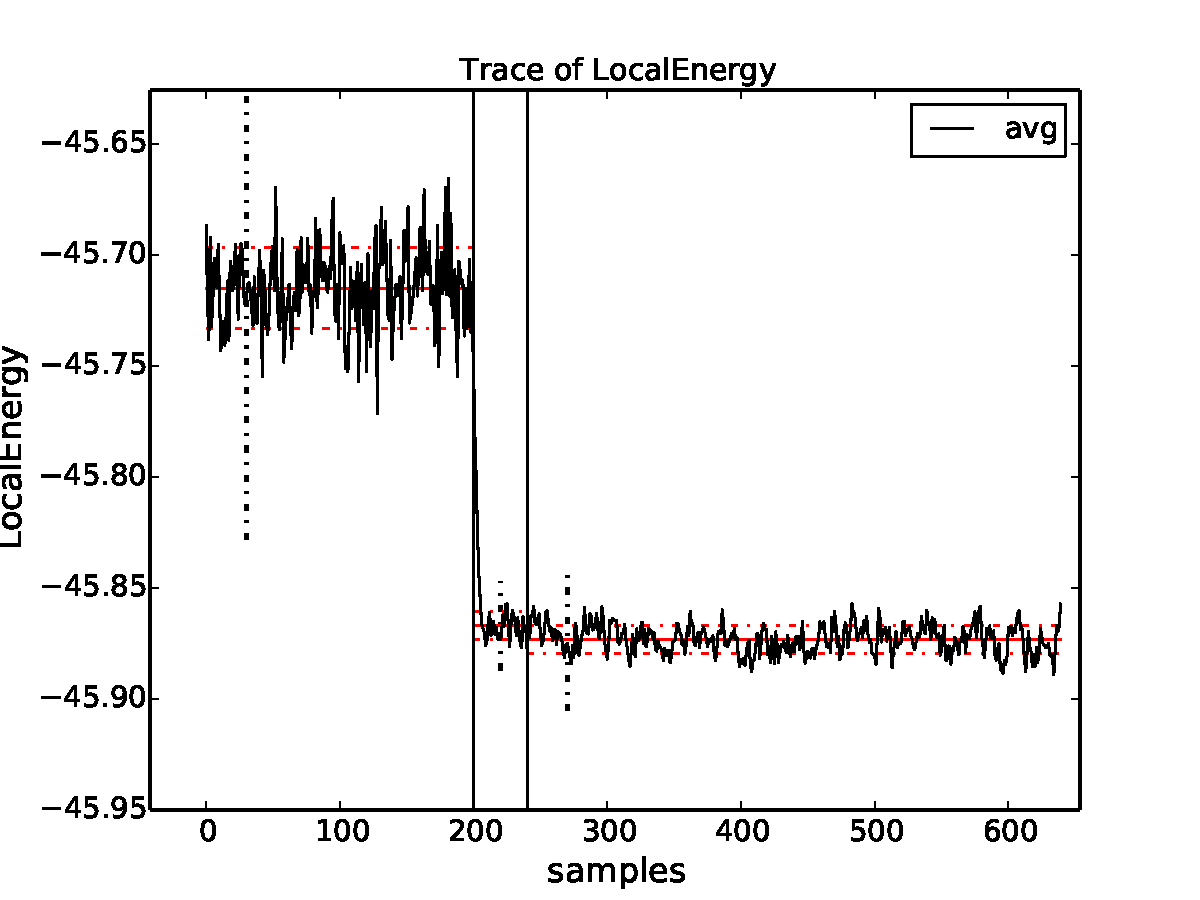
\includegraphics[trim = 0mm 0mm 0mm 0mm, clip,width=0.75\columnwidth]{figures/qmca_twist_average_trace.pdf}
\end{center}
\caption{Twist averaged energy trace from VMC to DMC for an 8 supercell of diamond obtained with \texttt{qmca}.  
\label{fig:qmca_twist_average}
}
\end{figure}

As can be seen from the Fig. \ref{fig:qmca_twist_overlap}, some of the twist 
angles are degenerate. This is seen more clearly in the text output:
\begin{shade}
>qmca -q ev -e 30 *s002.scalar*
                            LocalEnergy               Variance           ratio 
qmc.g000  series 2  -45.264510 +/- 0.001942   1.057065 +/- 0.002318   0.0234 
qmc.g001  series 2  -46.035511 +/- 0.001806   1.015992 +/- 0.002836   0.0221 
qmc.g002  series 2  -46.035410 +/- 0.001538   1.015039 +/- 0.002661   0.0220 
qmc.g003  series 2  -46.047285 +/- 0.001898   1.018219 +/- 0.002588   0.0221 
qmc.g004  series 2  -46.034225 +/- 0.002539   1.013420 +/- 0.002835   0.0220 
qmc.g005  series 2  -46.046731 +/- 0.002963   1.018337 +/- 0.004109   0.0221 
qmc.g006  series 2  -46.047133 +/- 0.001958   1.021483 +/- 0.003082   0.0222 
qmc.g007  series 2  -45.476146 +/- 0.002065   1.070456 +/- 0.003133   0.0235 
\end{shade}
\noindent
The degenerate twists grouped by set are $\{0\}$, $\{1,2,4\}$, $\{3,5,6\}$, 
$\{7\}$.

Alternatively, the run could have been performed at \emph{only} the four 
unique (irreducible) twist angles.  We will emulate this situation by 
analyzing data for twists 0, 1, 3, and 7 only.  In a production setting 
with irreducibly weighted twists, run would be performed on these twists 
alone; we reuse the uniform twist data for illustration purposes only.  

We can use \texttt{qmca} to perform twist averaging with different 
weights applied to each twist
\begin{shade}
>qmca -a -w '1 3 3 1' -q ev -e 30 *g000*2*sc* *g001*2*sc* *g003*2*sc* *g007*2*sc*
                            LocalEnergy               Variance           ratio 
avg  series 2  -45.873631 +/- 0.001044   1.028769 +/- 0.001520   0.0224 
\end{shade}
\noindent
yielding a total energy value of $-45.874(1)$ Ha, in agreement with the 
uniform weighted twist average performed above.  

The decision of whether or not to perform irreducible weighted twist 
averaging should be made on the basis of efficiency.  The relative 
efficiency of irreducible vs. uniform weighted twist averaging 
depends on the irreducible weights and the ratio of the lengths of 
the available sampling and equilibration periods.  A formula for 
the relative efficiency of these two cases is derived and discussed 
in more detail in Appendix \ref{sec:app_ta_efficiency}.


\subsection{Setting output units}
\label{sec:qmca_output_units}
Estimates outputted by \texttt{qmca} are in Hartree units by 
default.  The output units for energetic quantities can be 
changed by using the ``\texttt{-u}'' option.  

\vspace{3mm}
\noindent
Energy in Hartrees:
\begin{shade}
>qmca -q e -u Ha -e 20 qmc.s002.scalar.dat
qmc  series 2  LocalEnergy           =  -46.032960 +/- 0.002077
\end{shade}

\noindent
Energy in electron volts:
\begin{shade}
>qmca -q e -u eV -e 20 qmc.s002.scalar.dat
qmc  series 2  LocalEnergy           =  -1252.620565 +/- 0.056521 
\end{shade}

\noindent
Energy in Rydbergs:
\begin{shade}
>qmca -q e -u rydberg -e 20 qmc.s002.scalar.dat
qmc  series 2  LocalEnergy           =  -92.065919 +/- 0.004154   
\end{shade}

\noindent
Energy in kilojoules per mole:
\begin{shade}
>qmca -q e -u kj_mol -e 20 qmc.s002.scalar.dat
qmc  series 2  LocalEnergy           =  -120859.512998 +/- 5.453431   
\end{shade}


\subsection{Speeding up trace plotting}
\label{sec:qmca_fast_trace_plot}
When working with many files or files with many entries, 
\texttt{qmca} may take a long time to produce plots.  The time 
delay is actually due to the autocorrelation time estimate 
used to calculate error bars.  The calculation time for 
the autocorrelation scales as $\mathcal{O}(M^2)$, with $M$ being 
the number of statistical samples.  If you are only interested 
in plotting traces and not in the estimated error bars, the 
autocorrelation time estimation can be turned off with the 
``\texttt{--noac}'' option:
\begin{shade}
>qmca -t -q e -e 20 --noac qmc.s002.scalar.dat
\end{shade}
\noindent
Please note that the resulting error bars printed to the console 
will be underestimated and are not meaningful.  Do \emph{not} 
use ``\texttt{--noac}'' in conjunction with the ``\texttt{-p}'' 
plotting option as these plots are of no use without meaningful 
error bars.


\subsection{Short usage examples}
\label{sec:qmca_short_examples}
\noindent
Plotting a trace of the local energy:
\begin{shade}
>qmca -t -q e *scalar*
\end{shade}
\noindent
Applying an equilibration cutoff to VMC data (series 0):
\begin{shade}
>qmca -q e -e 30 *s000.scalar*
\end{shade}
\noindent
Applying the same equilibration cutoff to VMC and DMC data (series 0, 1, 2):
\begin{shade}
>qmca -q e -e 20 *scalar*
\end{shade}
\noindent
Applying different equilibration cutoffs to VMC and DMC data (series 0, 1, 2):
\begin{shade}
>qmca -q e -e '30 20 40' *scalar*
\end{shade}
\noindent
Obtaining the energy, variance, and variance/energy ratio for all series:
\begin{shade}
>qmca -q ev -e 30 *scalar*
\end{shade}
\noindent
Overlaying plots of mean + error bar for energy and variance for separate 
two- and three- body Jastrow optimization runs:
\begin{shade}
>qmca -po -q ev ./optJ2/*scalar* ./optJ3/*scalar*
\end{shade}
\noindent
Obtaining the acceptance ratio:
\begin{shade}
>qmca -q ar -e 30 *scalar*
\end{shade}
\noindent
Obtaining the average DMC walker population:
\begin{shade}
>qmca -q nw -e 400 *s002.dmc.dat
\end{shade}
\noindent
Obtaining the Monte Carlo efficiency:
\begin{shade}
>qmca -q eff -e 30 *scalar*
\end{shade}
\noindent
Obtaining the total wallclock time per series:
\begin{shade}
>qmca -q tt -e 0 *scalar*
\end{shade}
\noindent
Obtaining the average wallclock time spent per block:
\begin{shade}
>qmca -q bc -e 0 *scalar*
\end{shade}
\noindent
Obtaining a subset of desired quantities:
\begin{shade}
>qmca -q 'e v ar eff' -e 30 *scalar*
\end{shade}
\noindent
Obtaining all available quantities:
\begin{shade}
>qmca -e 30 *scalar*
\end{shade}
\noindent
Obtaining the twist averaged total energy with uniform weights:
\begin{shade}
>qmca -a -q e -e 40 *g*s002.scalar.dat
\end{shade}
\noindent
Obtaining the twist averaged total energy with specific weights:
\begin{shade}
>qmca -a -w '1 3 3 1' -q e -e 40 *g*s002.scalar.dat
\end{shade}
\noindent
Obtaining the local, kinetic, and potential energies in eV:
\begin{shade}
>qmca -q ekp -e 30 -u eV *scalar*
\end{shade}



\subsection{Production quality checklist}
\label{sec:qmca_production_checklist}

\begin{enumerate}
  \item{Inspect the trace plots (``\texttt{-t}'' option) for any 
    oddities in the data.  Typical behavior is a short equilibration 
    period followed by benign fluctuations around a clear mean value.  
    There should not be any large spikes in the data. This applies 
    to \emph{all} runs (VMC, optimization, DMC, etc.).}

  \item{Remove all equilibration steps (``\texttt{-e}'' option) from 
    the data by inspecting the trace plot.}

  \item{Check the quality of the orbitals (standalone Jastrow-less 
    VMC or sometimes the first \texttt{scalar} file produced during 
    optimization) by inspecting the variance/energy ratio 
    ``\texttt{qmca -q ev *scalar*}''.  For pseudopotential systems 
    without a Jastrow, the variance/energy ratio should not exceed 
    $0.2$ Ha, otherwise there is a problem with the orbitals.}

  \item{Check the quality of the optimized Jastrow factor by inspecting 
    the variance/energy ratio.  For pseudopotential systems with a 
    Jastrow, the variance/energy ratio should not exceed $0.04$ Ha 
    for pseudopotential systems.  A good Jastrow is indicated by a 
    variance/energy ratio in the range $0.01-0.03$ Ha.  A value less 
    than $0.01$ Ha is difficult to achieve.}

  \item{Confirm that the optimization has converged by plotting the 
    energy and variance vs. optimization series 
    (``\texttt{qmca -p -q ev *scalar*}'').  Do not assume that 
    optimization has converged in only a few cycles.  Use at least 
    10 cycles of with around 100,000 samples unless you already have 
    experience with the system in question.}

  \item{Optimize Jastrow factors according to energy minimization to 
    reduce locality errors arising from the use of non-local 
    pseudopotentials in DMC.  A good approach is to optimize with a 
    few cycles of variance minimization followed by several cycles of 
    energy minimization.}

  \item{Occasionally try optimizing with more samples and/or cycles 
    to see if improved results are obtained.}

  \item{If using a B-spline representation of the orbitals, converge 
    the VMC energy and variance with respect to the mesh size (controlled 
    via meshfactor).  This is best done in the presence of any 
    Jastrow factor to reduce noise.  Consider using the hybrid LMTO 
    representation of the orbitals as this can reduce both the VMC/DMC 
    variance and DMC timestep error in addition to saving memory.}

  \item{Check the variance/energy ratio of all production VMC and DMC 
    calculations.  In all cases the DMC ratio should be slightly 
    less than the VMC one and both should abide the guidelines above, 
    \emph{i.e.} the ratio should be less than $0.04$ Ha for 
    pseudopotential systems.  The production ratio should also be 
    consistent with what is observed during wavefunction optimization.}

  \item{Be aware of population control bias in DMC.  Run with a 
    population of $\sim 2000$ or greater.  Occasionally repeat a run 
    using a larger population to explicitly confirm that population 
    control bias is small.}

  \item{Check the stability of the DMC walker population by plotting 
    the trace of the population size (``\texttt{qmca -t -q nw *dmc.dat}'').  
    Verify that the average walker population is consistent with 
    the requested value provided in the input.}

  \item{In DMC, perform a timestep study to either 1) obtain 
    extrapolated results, or 2) obtain a timestep for future 
    production where an energy difference shows convergence 
    (\emph{e.g.} a band gap or defect formation energy).  For 
    pseudopotential systems, converged timesteps for many systems 
    are in the range $0.002-0.01$ Ha$^{-1}$, but the actual converged 
    timestep must be explicitly checked.}

  \item{In periodic systems, converge the total energy with respect to 
    the size of the twist/k-point grid.  Results for smaller systems 
    can easily be transferred to larger ones (\emph{e.g.} a 2x2x2 twist 
    grid in a 2x2x2 tiled cell is equivalent to a 1x1x1 twist grid in a 
    4x4x4 tiled cell)}.

  \item{In periodic systems, perform finite size extrapolation 
    including two body corrections (needed for cohesive energy/phase 
    stability studies) unless it can be shown that finite size effects 
    cancel for the energy difference in question (\emph{e.g.} some 
    defect formation energies).}

\end{enumerate}


\section{Using the qfit tool for statistical timestep extrapolation and curve fitting}
\label{sec:qfit}

The \texttt{qfit} tool is used to provide statistical estimates of
curve fitting parameters based on QMCPACK data.  While \texttt{qfit}
will eventually support many types of fitted curves (\emph{e.g.} Morse
potential binding curves, various equation of state fitting curves, etc.),
it is currently limited to estimating fitting parameters related to
timestep extrapolation.

\subsection{The jack-knife statistical technique}
The \texttt{qfit} tool obtains estimates of fitting parameter
means and associated error bars via the ``jack-knife''
technique.  The jack-knife method is a powerful and general tool
to obtain meaningful error bars for any quantity that is related
in a non-linear fashion to an underlying set of statistical data.
For this reason, we give a brief overview of the jack-knife
technique before proceeding with usage instructions for the
\texttt{qfit} tool.

Consider $N$ statistical variables $\{x_n\}_{n=1}^N$ that have
been outputted by one or more simulation runs.  If we have
$M$ samples of each of the $N$ variables, then the mean values
of each these variables can be estimated in the standard way,
i.e. $\bar{x}_n\approx \tfrac{1}{M}\sum_{m=1}^Mx_{nm}$.

Suppose we are interested in $P$ statistical quantities
$\{y_p\}_{p=1}^P$ that are related to the original $N$ variables
by a known multidimensional function $F$:
\begin{align}
  y_1,y_2,\ldots,y_P &= F(x_1,x_2,\ldots,x_N)\quad \textrm{or} \nonumber \\
  \vec{y} &= F(\vec{x})
\end{align}
The relationship implied by $F$ is completely general. 
For example the $\{x_n\}$ might be elements of a matrix
with $\{y_p\}$ being the eigenvalues, or $F$ might be
a fitting procedure for $N$ energies at different timesteps
with $P$ fitting parameters.  An approximate guess at the mean
value of $\vec{y}$ can be obtained by evaluating $F$ at the mean
value of $\vec{x}$ (i.e. $F(\bar{x}_1\ldots\bar{x}_N)$), but with
this approach we have no way to estimate the statistical error 
bar of any $\bar{y}_p$.

In the jack-knife procedure, the statistical variability intrinsic
to the underlying data $\{x_n\}$ is used to obtain estimates of the
mean and error bar of $\{y_p\}$.  We first construct a new set of $x$
statistical data by taking the average over all samples but one:
\begin{align}
  \tilde{x}_{nm} = \frac{1}{N-1}(N\bar{x}_n-x_{nm})\qquad m\in [1,M]
\end{align}
The result is a distribution of approximate $x$ mean values.  These
are used to construct a distribution of approximate means for $y$:
\begin{align}
  \tilde{y}_{1m},\ldots,\tilde{y}_{Pm} = F(\tilde{x}_{1m},\ldots,\tilde{x}_{Nm}) \qquad m\in [1,M]
\end{align}
Estimates for the mean and error bar of the quantities of
interest can finally be obtained using the formulas below:
\begin{align}
  \bar{y}_p &= \frac{1}{M}\sum_{m=1}^M\tilde{y}_{pm} \\
  \sigma_{y_p} &= \sqrt{\frac{M-1}{M}\left(\sum_{m=1}^M\tilde{y}_{pm}^2-M\bar{y}_p^2\right)}
\end{align}


\subsection{Performing timestep extrapolation}
In this section, we use a 32 atom supercell of MnO as an example
system for timestep extrapolation.  Data for this system has been
collected in DMC using the following sequence of timesteps:
$0.04,~0.02,~0.01,~0.005,~0.0025,~0.00125$ Ha$^{-1}$.  For a typical
production pseudopotential study, timesteps in the range
$0.02-0.002$ Ha$^{-1}$ are usually sufficient and it is recommended
to increase the number of steps/blocks by a factor of two when
the timestep is halved.  In order to perform accurate statistical
fitting, we must first understand the equilibration and autocorrelation
properties of the inputted local energy data.  After plotting the
local energy traces (\texttt{qmca -t -q e -e 0 ./qmc*/*scalar*})
it is clear that an equilibration period of $30$ blocks is reasonable.
Approximate autocorrelation lengths are also obtained with \texttt{qmca}:
\begin{shade}
>qmca -e 30 -q e --sac ./qmc*/qmc.g000.s002.scalar.dat
./qmc_tm_0.00125/qmc.g000 series 2 LocalEnergy = -3848.234513 +/- 0.055754  1.7 
./qmc_tm_0.00250/qmc.g000 series 2 LocalEnergy = -3848.237614 +/- 0.055432  2.2 
./qmc_tm_0.00500/qmc.g000 series 2 LocalEnergy = -3848.349741 +/- 0.069729  2.8 
./qmc_tm_0.01000/qmc.g000 series 2 LocalEnergy = -3848.274596 +/- 0.126407  3.9 
./qmc_tm_0.02000/qmc.g000 series 2 LocalEnergy = -3848.539017 +/- 0.075740  2.4 
./qmc_tm_0.04000/qmc.g000 series 2 LocalEnergy = -3848.976424 +/- 0.075305  1.8 
\end{shade}
\noindent
The autocorrelation must be removed from the data prior to jack-knifing
and so we will reblock the data by a factor of 4.

The \texttt{qfit} tool can be used in the following way to obtain
a linear timestep fit of the data:
\begin{shade}
>qfit ts -e 30 -b 4 -s 2 -t '0.00125 0.0025 0.005 0.01 0.02 0.04' ./qmc*/*scalar*
fit function  : linear
fitted formula: (-3848.193 +/- 0.037) + (-18.95 +/- 1.95)*t
intercept     : -3848.193 +/- 0.037  Ha
\end{shade}
The input arguments are as follows: \texttt{ts} indicates we are
performing a timestep fit, ``\texttt{-e 30}'' is the equilibration period
removed from each set of scalar data, ``\texttt{-b 4}'' indicates the data
will be reblocked by a factor of 4 (\emph{e.g.} a file containing 400 \
entries will be block averaged into a new set of 100 prior to jack-knife
fitting), ``\texttt{-s 2}'' indicates that the timestep data begins with
series 2 (scalar files matching \texttt{*s000*} or \texttt{*s001*} are
to be excluded), and ``\texttt{-t } '0.00125 0.0025 0.005 0.01 0.02 0.04' ''
provides a list of timestep values corresponding to the inputted scalar
files.  The ``\texttt{-e}'' and ``\texttt{-b}'' options can receive a
list of file-specific values (same format as ``\texttt{-t}'') if desired.
As can be seen from the text output, the parameters for the linear fit
are printed with error bars obtained with jack-knife resampling and
the zero timestep ``intercept'' is $-3848.19(4)$ Ha.  In addition to
text output, the command above will result in a plot of the fit with
the zero timestep value shown as a red dot, as shown in the left
panel of Fig.~\ref{fig:qfit_timestep}.

\begin{figure}
  \centering
  \begin{subfigure}[t]{0.47\textwidth}
    \centering
    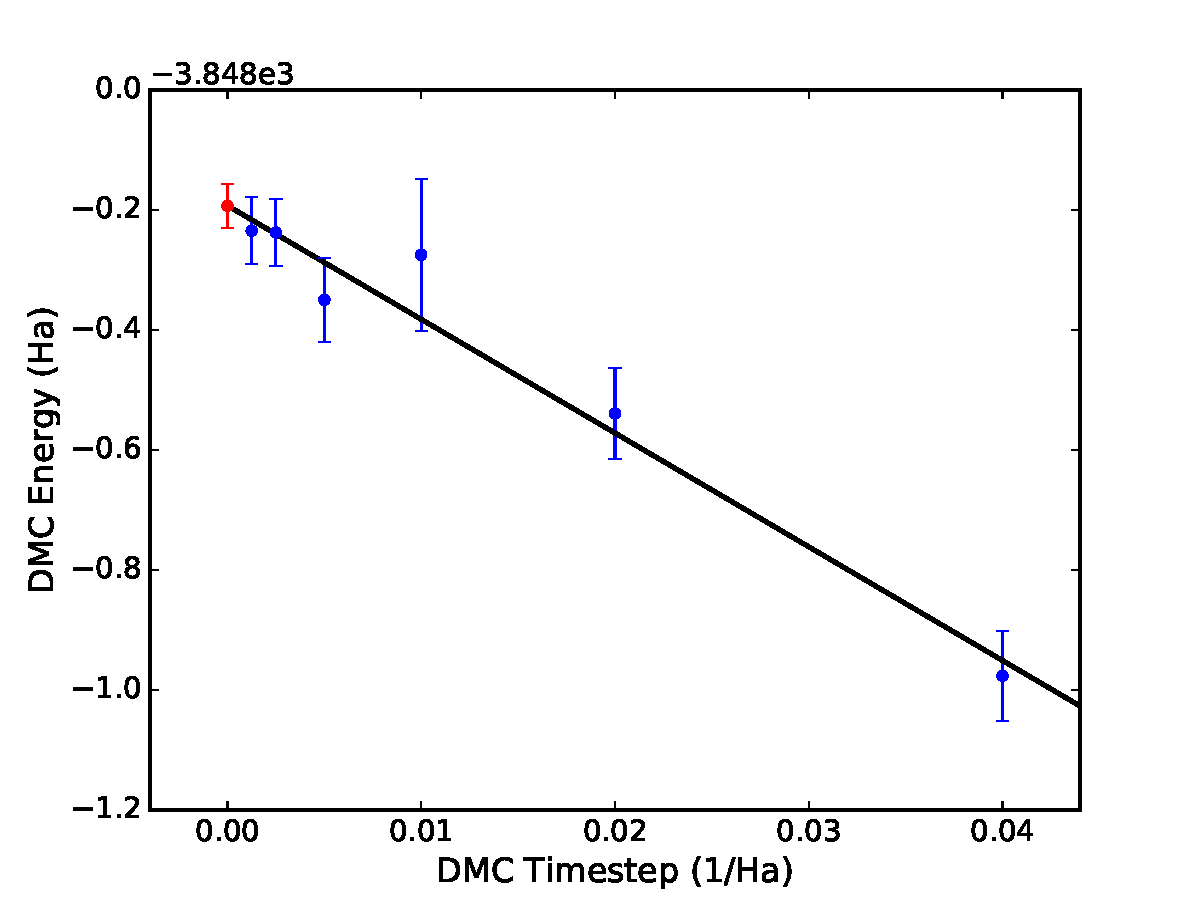
\includegraphics[trim=0mm 0mm 4mm 0mm,clip,width=\linewidth]{figures/qfit_timestep_linear.pdf}
  \end{subfigure}
  \begin{subfigure}[t]{0.47\textwidth}
    \centering
    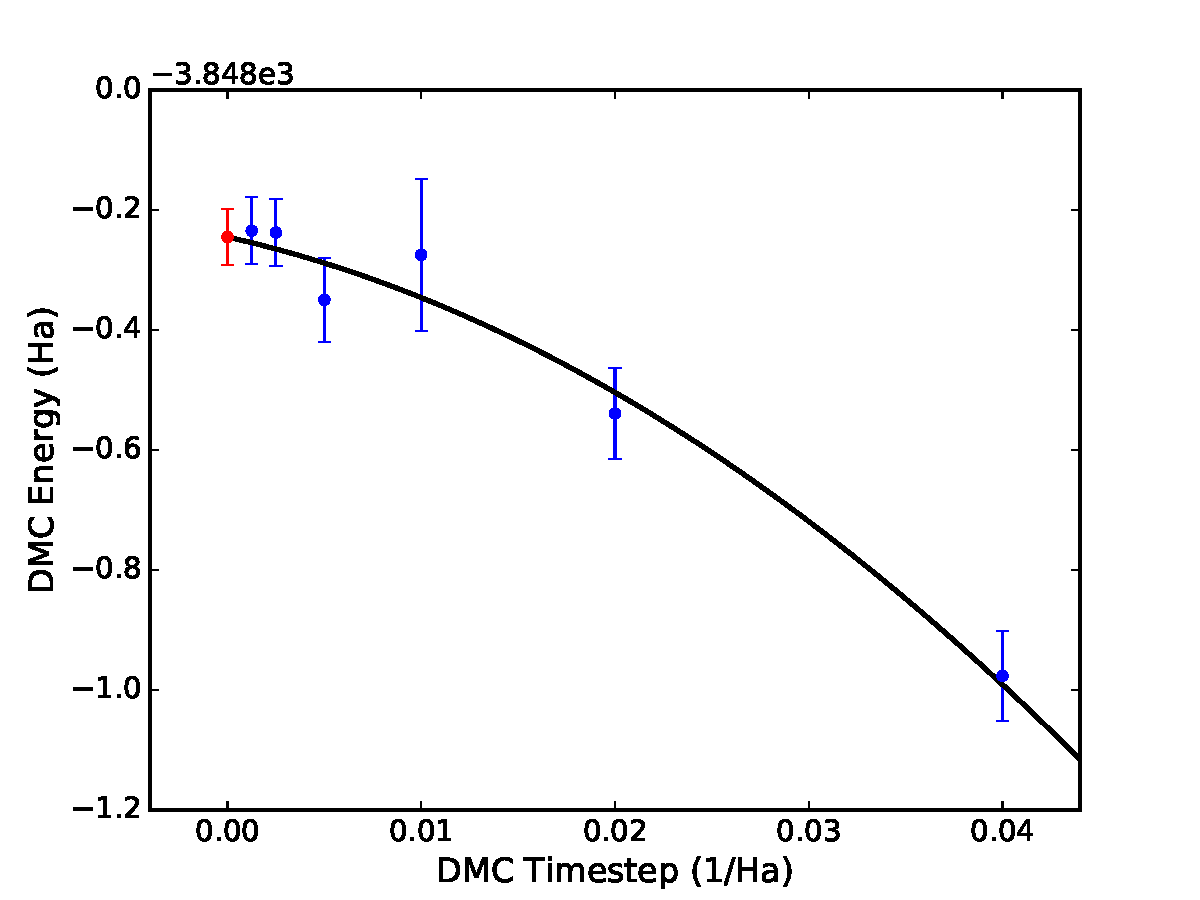
\includegraphics[trim=2mm 0mm 4mm 0mm,clip,width=\linewidth]{figures/qfit_timestep_quadratic.pdf}
  \end{subfigure}
  \caption{Linear (left) and quadratic (right) timestep fits to DMC data for a 32 atom supercell of MnO obtained with \texttt{qfit}.  Zero timestep estimates are indicated by the red data point on the left side of either panel.\label{fig:qfit_timestep}}
\end{figure}

Different fitting functions are supported via the ``\texttt{-f}'' option.
Currently supported options include \texttt{linear} ($a+bt$),
\texttt{quadratic} ($a+bt+ct^2$), and \texttt{sqrt} ($a+b\sqrt{t}+ct$).
Results for a quadratic fit are shown below as well as in the right
panel of Fig.~\ref{fig:qfit_timestep}.
\begin{shade}
>qfit ts -f quadratic -e30 -b4 -s2 -t '0.00125 0.0025 0.005 0.01 0.02 0.04' ./qmc*/*scalar*
fit function  : quadratic
fitted formula: (-3848.245 +/- 0.047) + (-7.25 +/- 8.33)*t + (-285.00 +/- 202.39)*t^2
intercept     : -3848.245 +/- 0.047  Ha
\end{shade}
In this case we find a zero timestep estimate of $-3848.25(5)$ Ha$^{-1}$.
A timestep of $0.04$ Ha$^{-1}$ might be on the large side to include in
timestep extrapolation and it is likely to have an outsize influence
in the case of linear extrapolation.  Upon excluding this point, linear
extrapolation yields a zero timestep value of $-3848.22(4)$ Ha$^{-1}$.
It should be noted that quadratic extrapolation can result in intrinsically
larger uncertainty in the extrapolated value.  For example, when the $0.04$
Ha$^{-1}$ point is excluded the uncertainty grows by 50\% and we obtain an
estimated value of $-3848.28(7)$ instead.



\section{Densities and spin-densities}
\label{sec:densities}

\section{Energy densities}
\label{sec:energydensities}




\input{examples}

% labs: import each as a separate chapter for now
\input{lab_qmc_statistics}
\input{lab_qmc_basics}
\input{lab_advanced_molecules}
\input{lab_condensed_matter}


\chapter{Additional Tools}
\label{chap:additional_tools}
QMCPACK provides a set of lightweight executables that address certain
common problems in QMC workflow and analysis.  These range from conversion utilities between 
different file formats and QMCPACK (e.g. ppconvert and convert4qmc),  
(extract-eshdf-kvectors), to post-processing utilities (trace-density and qmcfinitesize), and to many others.  In this chapter, we cover the use cases, syntax, and features of all additional tools provided with QMCPACK.  

\section{Initialization Tools}
  \subsection{getSupercell}

\section{Post-Processing}
  \subsection{qmca}
    qmca is a versatile tool to analyze and plot the raw data from QMCPACK *.scalar.dat files.
    It is a python executable and part of the Nexus suite of tools.  It can be found in 
    \texttt{trunk/nexus/executables}. 
  \subsection{qmcfit}
  \subsection{qmcfinitesize}
    qmcfinitesize is a utility to compute many-body finite-size corrections to the energy.  It
    is a C++ executable that is built alongside the qmcpack executable.  It can be found in 
    \texttt{trunk/build/bin}
  \subsection{trace-density}

\section{Converters} 
  \subsection{convert4qmc}
    convert4qmc allows conversion of orbitals and wavefunctions from quantum chemistry
    output files to QMCPACK xml input files.  It is a small C++ executable that is built 
    alongside the qmcpack executable, and can be found in \texttt{trunk/build/bin}.  
  \subsection{wfconvert}
    wfconvert allow conversion between 
  \subsection{pw2qmcpack.x}
    pw2qmcpack.x is an executable that converts PWSCF wavefunctions to QMCPACK readable 
    HDF5 format.  This utility is built alongside the Quantum Espresso post-processing utilities.
    This utility is written in Fortran90, and is distributed as a patch of the Quantum Espresso 
    source code.  The patch, as well as automated QE download and patch scripts, can be found in 
    \texttt{trunk/external\_codes/quantum\_espresso}.
  \subsection{ppconvert}
    ppconvert is a utility to convert pseudopotentials between different commonly used formats.
    It is a stand alone C++ executable that is not automatically built, but the source is 
    included in \texttt{trunk/src/QMCTools/ppconvert}.  BLAS/LAPACK libraries are required.  

\section{Miscellaneous}
  \subsection{extract-eshdf-kvectors}
    


\input{unit_testing}
\input{contributing}

\newpage
\chapter{References}
%\begingroup  % Avoid "References" section title
%\renewcommand{\section}[2]{}%
\bibliographystyle{ieeetr}
\bibliography{bibliography}
%\endgroup

\end{document}
